%==============================================================================
% Jarvis-HEP — The Complete User & Reference Manual
% Master file.  Build:  latexmk -pdf main.tex   (pdfLaTeX + biber)
%
% Class: tufte-book (kept by design decision 2026-06-13).
%   - hyperref ENABLED (no 'nohyper') for clickable cross-refs + PDF bookmarks.
%   - 'nobib' so we drive the bibliography with biblatex+biber ourselves.
% Structure lives in style/ (preamble, listings, boxes) and chapters/.
% Drafting tip: uncomment \includeonly{...} to compile a single chapter fast.
%==============================================================================
% symmetric -> sidenote/margin on the OUTER edge, mirrored on odd/even pages
%             (implies twoside; the outer margin is left blank for notes).
% openany   -> chapters start on the next page (no blank pages between chapters);
%             part dividers are restored to a recto start below.
\documentclass[symmetric,openany,nobib]{tufte-book}

% --- Shared setup -------------------------------------------------------------
%==============================================================================
% jarvis-preamble.tex
% Shared packages, metadata macros, and semantic text commands for the
% Jarvis-HEP manual.  Loaded by main.tex after \documentclass{tufte-book}.
%
% The tufte-book class already provides: xcolor, hyperref (unless nohyper),
% geometry, graphicx, \allcaps, \smallcaps, \newthought, \sidenote,
% \marginnote, \footnote->sidenote, fullwidth env, marginfigure, etc.
% We only add what a code/reference manual additionally needs.
%==============================================================================

% --- Math ---------------------------------------------------------------------
\usepackage{amsmath}
\usepackage{amssymb}

% --- Tables -------------------------------------------------------------------
\usepackage{booktabs}
\usepackage{longtable}
\usepackage{array}
\usepackage{ragged2e}      % \RaggedRight inside narrow table cells

% --- Misc ---------------------------------------------------------------------
\usepackage{pmboxdraw}     % render block/box-drawing glyphs (the Jarvis -v banner) in pdfLaTeX
\usepackage{newunicodechar} % map the literal dot glyph U+2B24 (the banner icon) to a drawn circle
\usepackage{varwidth}      % shrink-to-content box so the banner panel hugs its text (no empty margin)
\usepackage{xspace}        % smart trailing space for text macros
\usepackage{enumitem}      % tighter description/itemize lists
\setlist{noitemsep, topsep=2pt}

% --- Project version single-source --------------------------------------------
% This manual is a LIVING document: it is revised in step with each Jarvis-HEP
% release.  \JversionNum names the release this particular build documents --
% bump it (and rebuild) on every release; do not hard-code version numbers in
% the prose, always use \Jversion so there is a single source of truth.
\newcommand{\JversionNum}{1.7.3}
\newcommand{\Jversion}{v\JversionNum\xspace}

% --- Product / ecosystem names ------------------------------------------------
\newcommand{\Jarvis}{\textsc{Jarvis-HEP}\xspace}
\newcommand{\Operas}{\textsc{Jarvis-Operas}\xspace}
\newcommand{\JPlot}{\textsc{Jarvis-PLOT}\xspace}

% --- Inline semantic markup ---------------------------------------------------
% Monospace helper that lets long tokens break in the narrow text column: an
% underscore (\_) and a dot offer a zero-penalty breakpoint, so names like
% interpolations\_1D or Runtime.batch\_size can wrap instead of overflowing.
\newcommand{\jbttbreak}{\penalty0\hskip0pt\relax}
\newcommand{\jtt}[1]{\begingroup
  \def\_{\textunderscore\jbttbreak}%
  \texttt{#1}\endgroup}
% Code-ish things rendered in monospace with consistent meaning across the book.
\newcommand{\code}[1]{\jtt{#1}}                          % generic inline code
\newcommand{\yamlkey}[1]{\jtt{#1}}                       % a YAML key / block name
\newcommand{\cli}[1]{\jtt{#1}}                           % a shell / CLI fragment
\newcommand{\token}[1]{\jtt{#1}}                         % runtime token @SampleID etc.
\newcommand{\marker}[1]{\jtt{#1}}                        % path marker &J/
\newcommand{\file}[1]{\jtt{#1}}                          % a file or path (overridden in dirtree)
\newcommand{\sampler}[1]{\textsf{#1}}                    % a sampler method name
\newcommand{\optitem}[1]{\textit{#1}}                    % an "(optional)" tag etc.

% Reference to a sampler JSON schema file (authoritative key source).
\newcommand{\schemaref}[1]{\texttt{card/schema/#1}}

% A "registered alias" inline note, e.g. \alias{ToyMCMC}{MCMC}
\newcommand{\alias}[2]{\texttt{#1}~(alias of~\texttt{#2})}

% --- Required / Optional inline tags for key tables ---------------------------
\newcommand{\req}{\textbf{required}}
\newcommand{\opt}{optional}

% --- Tufte: \paragraph is our de-facto third heading level --------------------
% tufte-book forbids \subsubsection, so \paragraph (provided by the class) is the
% deepest heading we use.  We deliberately do NOT redefine it, to avoid clashing
% with the class's titlesec-based sectioning.

% --- A compact key/value description list for YAML key references -------------
\newenvironment{keylist}
  {\begin{description}[style=nextline, leftmargin=1.2em, font=\ttfamily]}
  {\end{description}}

% --- Coloured cross-reference & citation links --------------------------------
% tufte loads hyperref with colorlinks=false (links are black, box-less), so
% references look like plain text.  Turn on coloured links so references to
% figures, tables, equations, and sections -- and citations -- stand out.
% (hyperref is already loaded by the tufte-book class at this point.)
\definecolor{jlink}{HTML}{1F6FB2}  % cross-refs: figures, tables, equations, sections
\definecolor{jcite}{HTML}{2E7D32}  % citations / bibliography
\definecolor{jurl}{HTML}{1A5FB4}   % URLs
\hypersetup{
  colorlinks = true,
  linkcolor  = jlink,
  citecolor  = jcite,
  urlcolor   = jurl,
  linktoc    = page,   % keep ToC titles black; colour only the page-number links
}

%==============================================================================
% jarvis-listings.tex
% Code-listing setup for the Jarvis-HEP manual.
%
% Provides:
%   - a Jarvis color palette
%   - a custom YAML language definition (listings has none built in)
%   - styles:  yaml   (task-card YAML)
%              bash   (shell / CLI sessions)
%              plain  (generic / SLHA / output dumps)
%   - convenience inline/float macros
%
% Long real-world cards should be \lstinputlisting'd from ../listings/ so they
% stay byte-true with jarvishep/project_template.  Inside Tufte's narrow text
% column, wrap wide listings in a {fullwidth} environment.
%==============================================================================

\usepackage{listings}

% --- Palette ------------------------------------------------------------------
\definecolor{jBg}{HTML}{F7F7F4}      % listing background
\definecolor{jRule}{HTML}{D8D8D0}    % frame rule
\definecolor{jKey}{HTML}{1F4E79}     % YAML keys / keywords (deep blue)
\definecolor{jStr}{HTML}{8A5A00}     % strings (amber)
\definecolor{jComment}{HTML}{6E7B6E} % comments (muted green-grey)
\definecolor{jNum}{HTML}{7A1F8B}     % numbers (purple)
\definecolor{jMarker}{HTML}{B3261E}  % &J/ @tokens / ${...} (Jarvis red)
\definecolor{jLineNo}{HTML}{A0A0A0}
\definecolor{jLineNum}{HTML}{C7CCD2}  % very light grey for YAML line numbers
\definecolor{jGuide}{HTML}{E3E6EA}    % very light grey for YAML indentation guides

% --- Semantic colours (used inline and in listings) ---------------------------
\definecolor{jExpr}{HTML}{C2185B}     % expressions  -> pink
\definecolor{jPath}{HTML}{1B5E20}     % file/dir paths -> dark green
\definecolor{jCmd}{HTML}{E8730C}      % Jarvis CLI commands -> Jarvis orange

% --- Inline semantic markup ---------------------------------------------------
\newcommand{\expr}[1]{\textcolor{jExpr}{\jtt{#1}}}   % an expression, e.g. \expr{x * Pi}
\newcommand{\cmd}[1]{\textcolor{jCmd}{\jtt{#1}}}     % a Jarvis CLI command, e.g. \cmd{Jarvis}

% --- A minimal YAML dialect ---------------------------------------------------
% Good enough to colour keys, strings, comments, booleans, and Jarvis markers
% without a full parser.
\lstdefinelanguage{jyaml}{
  morekeywords={true,false,null,True,False,None,yes,no},
  sensitive=true,
  morecomment=[l]{\#},
  morestring=[b]",
  morestring=[b]',
  alsoletter={-,_,.},
}

% --- Shared base style --------------------------------------------------------
\lstdefinestyle{jbase}{
  backgroundcolor=\color{jBg},
  basicstyle=\ttfamily\footnotesize,
  breaklines=true,
  breakatwhitespace=false,
  postbreak=\mbox{\textcolor{jLineNo}{$\hookrightarrow$}\space},
  columns=fullflexible,
  keepspaces=true,
  showstringspaces=false,
  tabsize=2,
  frame=leftline,
  framerule=1.2pt,
  rulecolor=\color{jRule},
  xleftmargin=0.8em,
  framexleftmargin=0.8em,
  aboveskip=0.9\baselineskip,
  belowskip=0.6\baselineskip,
}

% --- YAML style ---------------------------------------------------------------
\lstdefinestyle{yaml}{
  style=jbase,
  language=jyaml,
  keywordstyle=\color{jNum}\bfseries,   % booleans/null
  stringstyle=\color{jStr},
  commentstyle=\color{jComment}\itshape,
  % Highlight Jarvis markers and tokens.
  moredelim=[is][\color{jMarker}\bfseries]{@@}{@@},
  % Very light line numbers in the left margin (outside the frame rule).
  numbers=left,
  numberstyle=\tiny\color{jLineNum},
  numbersep=9pt,
  xleftmargin=2.6em,
  framexleftmargin=2.6em,
}

% --- Bash / CLI style ---------------------------------------------------------
\lstdefinestyle{bash}{
  style=jbase,
  language=bash,
  keywordstyle=\color{jKey}\bfseries,
  commentstyle=\color{jComment}\itshape,
  stringstyle=\color{jStr},
  morekeywords={Jarvis,pip,python3,cd,latexmk},
}

% --- Plain dump style (SLHA blocks, output text) ------------------------------
\lstdefinestyle{plain}{
  style=jbase,
  language={},
  keywordstyle=\color{jKey},
  commentstyle=\color{jComment}\itshape,
}

% --- Inner style for the boxed shell environment (frame/bg come from the box) --
\lstdefinestyle{shellinner}{
  language=bash,
  basicstyle=\ttfamily\footnotesize,
  keywordstyle=\color{jKey}\bfseries,
  commentstyle=\color{jComment}\itshape,
  stringstyle=\color{jStr},
  morekeywords={pip,python3,cd,source,pyenv,latexmk,make},
  keywords=[2]{Jarvis,jplot,jopera},        % Jarvis-family executables
  keywordstyle=[2]\color{jCmd}\bfseries,     % ... in Jarvis orange
  breaklines=true,
  postbreak=\mbox{\textcolor{jLineNo}{$\hookrightarrow$}\space},
  columns=fullflexible, keepspaces=true, showstringspaces=false, tabsize=2,
  aboveskip=0pt, belowskip=0pt,   % no extra listing space inside the box
}

% --- YAML style for the "window" box (frame/background come from the box) ------
% Line numbers (very light), expression values in pink, &J paths in dark green.
\lstdefinestyle{yamlwindow}{
  language=jyaml,
  basicstyle=\ttfamily\footnotesize,
  keywordstyle=\color{jNum}\bfseries,
  commentstyle=\color{jComment}\itshape,
  morestring=[b]", stringstyle=\color{jStr},
  moredelim=[s][\color{jExpr}]{expression: "}{"},
  moredelim=[l][\color{jPath}]{"\&J},
  numbers=left, numberstyle=\tiny\color{jLineNum}, numbersep=12pt,
  xleftmargin=2.4em,
  breaklines=true, columns=fullflexible, keepspaces=true, showstringspaces=false, tabsize=2,
  aboveskip=0pt, belowskip=0pt,
}

\lstset{style=jbase}

% --- Convenience environments / macros ----------------------------------------
% \begin{yamlcode} ... \end{yamlcode}
\lstnewenvironment{yamlcode}{\lstset{style=yaml}}{}
% \begin{bashcode} ... \end{bashcode}
\lstnewenvironment{bashcode}{\lstset{style=bash}}{}
% \begin{plaincode} ... \end{plaincode}
\lstnewenvironment{plaincode}{\lstset{style=plain}}{}

% File include shortcuts (keep wide ones inside {fullwidth}).
\newcommand{\yamlfile}[1]{\lstinputlisting[style=yaml]{#1}}
\newcommand{\bashfile}[1]{\lstinputlisting[style=bash]{#1}}

% Inline monospace shortcut already provided as \code in the preamble.

%==============================================================================
% jarvis-boxes.tex
% Admonition boxes for the Jarvis-HEP manual, built on tcolorbox.
%
% Four flavours, used sparingly (see the style guide in the writing plan):
%   \begin{jnote} ... \end{jnote}        general clarification
%   \begin{jtip} ... \end{jtip}          best-practice advice
%   \begin{jwarn} ... \end{jwarn}        foot-guns / things that bite
%   \begin{jschema}{File_schema.json} ... \end{jschema}
%                                        "verify these keys against the schema"
%
% Boxes are sized to the Tufte text column.  For a full-width box, wrap the
% environment in {fullwidth}.
%==============================================================================

\usepackage[most]{tcolorbox}

% Reuse the palette defined in jarvis-listings.tex.
\providecolor{jNote}{HTML}{1F4E79}
\providecolor{jTip}{HTML}{2E7D32}
\providecolor{jWarn}{HTML}{B3261E}
\providecolor{jSchema}{HTML}{6A1B9A}

\tcbset{
  jbox/.style={
    enhanced, breakable,
    boxrule=0pt, leftrule=2.5pt,
    arc=1pt, outer arc=1pt,
    left=8pt, right=6pt, top=5pt, bottom=5pt,
    fonttitle=\sffamily\bfseries\footnotesize,
    fontupper=\small,
    before skip=0.8\baselineskip, after skip=0.8\baselineskip,
  }
}

% Title bar: a LIGHT tint of the accent colour, with the accent itself as the
% (dark) title text -- so the heading reads but is no longer a heavy dark band.
\newtcolorbox{jnote}{%
  jbox, colback=jNote!4, colframe=jNote,
  colbacktitle=jNote!15, coltitle=jNote!90!black,
  title={Note}}

\newtcolorbox{jtip}{%
  jbox, colback=jTip!5, colframe=jTip,
  colbacktitle=jTip!15, coltitle=jTip!90!black,
  title={Tip}}

\newtcolorbox{jwarn}{%
  jbox, colback=jWarn!5, colframe=jWarn,
  colbacktitle=jWarn!15, coltitle=jWarn!90!black,
  title={Warning}}

% Schema-check box takes the schema file name as a mandatory argument.
\newtcolorbox{jschema}[1]{%
  jbox, colback=jSchema!4, colframe=jSchema,
  colbacktitle=jSchema!15, coltitle=jSchema!90!black,
  title={Verify against \texttt{#1}}}

%==============================================================================
% Shell-command box: a terminal-styled wrapper for CLI snippets, matching the
% call-out boxes above (light title bar + accent left rule + light body).
% Uses tcblisting (listings engine) with the `shellinner' style from
% jarvis-listings.tex; \faTerminal is provided by fontawesome5 (loaded later but
% expanded only at use time).  Use \begin{shellbox} ... \end{shellbox}.
%==============================================================================
\definecolor{jShell}{HTML}{334155}   % terminal slate

%==============================================================================
% YAML "window" box: a GUI-editor look for YAML listings -- a title bar with
% traffic-light dots and a filename, faint indentation guides, and light line
% numbers.  Use \begin{yamlwin}[filename] ... \end{yamlwin} (the optional title
% defaults to "YAML").  The yamlwindow style (jarvis-listings.tex) colours
% expression values pink and &J paths dark green.
%==============================================================================
\definecolor{jWinFrame}{HTML}{CDD2D8}  % window border
\definecolor{jWinBar}{HTML}{ECEEF1}    % title-bar background
\definecolor{jWinTitle}{HTML}{5A6470}  % title-bar text
\definecolor{tlRed}{HTML}{FF5F56}
\definecolor{tlYel}{HTML}{FFBD2E}
\definecolor{tlGrn}{HTML}{27C93F}
\newcommand{\trafficlights}{\tikz[baseline=-0.6ex]{%
  \fill[tlRed](0,0)circle(2.1pt);\fill[tlYel](7pt,0)circle(2.1pt);\fill[tlGrn](14pt,0)circle(2.1pt);}}

\newtcblisting{yamlwin}[1][YAML]{%
  enhanced, breakable,
  colback=jBg, colframe=jWinFrame,
  boxrule=0.7pt, arc=4pt, outer arc=4pt,
  boxsep=0pt, left=4pt, right=5pt, top=5pt, bottom=5pt,
  colbacktitle=jWinBar, coltitle=jWinTitle,
  fonttitle=\sffamily\footnotesize,
  toptitle=4pt, bottomtitle=4pt,
  title={\trafficlights\hspace{0.8em}{\ttfamily\footnotesize #1}},
  before skip=0.9\baselineskip, after skip=0.9\baselineskip,
  % faint vertical indentation guides (one per 2-space level), like an editor
  underlay={\begin{tcbclipinterior}\foreach \k in {1,...,7}{%
    \draw[jGuide,line width=0.4pt]
      ([xshift=2.4em+\k*1em]interior.north west)--([xshift=2.4em+\k*1em]interior.south west);}%
    \end{tcbclipinterior}},
  listing only,
  listing options={style=yamlwindow},
}

\newtcblisting{shellbox}{%
  enhanced, breakable,
  boxrule=0pt, leftrule=2.5pt, arc=1pt, outer arc=1pt,
  boxsep=0pt, left=8pt, right=6pt, top=4pt, bottom=4pt,
  colback=jShell!4, colframe=jShell,
  colbacktitle=jShell!15, coltitle=jShell!90!black,
  fonttitle=\sffamily\bfseries\footnotesize,
  toptitle=3.5pt, bottomtitle=3.5pt,
  title={\raisebox{-0.2pt}{\scalebox{0.8}{\faTerminal}}\ \ Shell},
  before skip=0.8\baselineskip, after skip=0.8\baselineskip,
  listing only,
  listing options={style=shellinner},
}

%==============================================================================
% jarvis-dirtree.tex
% Pretty directory trees for the manual, built on dirtree + fontawesome5.
%
% pdfLaTeX cannot render colour emoji (those need LuaLaTeX/XeLaTeX), so we use
% FontAwesome 5 glyphs coloured in the Jarvis palette as folder/file icons.
%
% ICON STYLE: outline only ("regular"), never filled ("solid").  Every icon below
% uses the [regular] variant.  Note that FontAwesome 5 *Free* ships only a limited
% regular set: file-csv and file-contract are solid-only, so CSV uses the outline
% spreadsheet glyph and there is no contract icon here.
%
% Usage:
%   \begin{jfiletree}
%   \dirtree{%
%     .1 \dtfold{MyScan/}.
%     .2 \dtfold{bin/}.
%     .3 \dtyaml{task.yaml}.
%     .2 \dtmark{.jarvis-project.json}\DTcomment{project marker}.
%   }
%   \end{jfiletree}
%
% \DTcomment{...} adds a right-aligned, dotted-leader annotation.
%==============================================================================

\usepackage{dirtree}
\usepackage{fontawesome5}

% Icon colours (Jarvis palette).
\definecolor{jfolder}{HTML}{75A3FA}   % folders: Jarvis blue
\definecolor{jfileicon}{HTML}{7B8794} % files: neutral slate
\definecolor{jmarkicon}{HTML}{B3261E} % project markers: Jarvis red

% Generic builder: an outline (regular) icon in a colour, then the monospace name.
\newcommand{\dticon}[2]{\textcolor{#1}{#2}\hspace{0.45em}}

% --- Folders (Jarvis blue) ----------------------------------------------------
\newcommand{\dtfold}[1]{\dticon{jfolder}{\faFolder[regular]}\texttt{#1}}
\newcommand{\dtfoldopen}[1]{\dticon{jfolder}{\faFolderOpen[regular]}\texttt{#1}}

% --- Typed files (neutral slate) ----------------------------------------------
\newcommand{\dtfile}[1]{\dticon{jfileicon}{\faFile[regular]}\texttt{#1}}        % generic file
\newcommand{\dtcode}[1]{\dticon{jfileicon}{\faFileCode[regular]}\texttt{#1}}     % yaml/json/config/script
\newcommand{\dtjson}[1]{\dticon{jfileicon}{\faFileCode[regular]}\texttt{#1}}     % json (alias of \dtcode)
\newcommand{\dtcsv}[1]{\dticon{jfileicon}{\faFileExcel[regular]}\texttt{#1}}     % csv / tabular data
\newcommand{\dtdata}[1]{\dticon{jfileicon}{\faChartBar[regular]}\texttt{#1}}     % hdf5 / results data
\newcommand{\dtdoc}[1]{\dticon{jfileicon}{\faFile[regular]}\texttt{#1}}          % readme / markdown / text
\newcommand{\dtimage}[1]{\dticon{jfileicon}{\faFileImage[regular]}\texttt{#1}}   % image / plot
\newcommand{\dtpdf}[1]{\dticon{jfileicon}{\faFilePdf[regular]}\texttt{#1}}       % pdf
\newcommand{\dtarchive}[1]{\dticon{jfileicon}{\faFileArchive[regular]}\texttt{#1}} % tar.gz / zip
\newcommand{\dtnote}[1]{\dticon{jfileicon}{\faStickyNote[regular]}\texttt{#1}}   % note

% --- Project markers (Jarvis red) ---------------------------------------------
\newcommand{\dtmark}[1]{\dticon{jmarkicon}{\faFile[regular]}\texttt{#1}}         % .jarvis-project.json
\newcommand{\dtyaml}[1]{\dticon{jmarkicon}{\faFileCode[regular]}\texttt{#1}}     % jarvis.project.yaml marker

% Width-constrained wrapper so dirtree lays out inside the text column (its
% dotted \DTcomment leaders run to the column's right edge).
\newenvironment{jfiletree}
  {\par\addvspace{0.6\baselineskip}\noindent\begin{minipage}{\linewidth}\footnotesize}
  {\end{minipage}\par\addvspace{0.6\baselineskip}}

%==============================================================================
% Inline file/folder mentions.
% \file{...} (defined plain in jarvis-preamble.tex) is upgraded here to prepend
% the matching outline icon, so EVERY inline file/folder reference in the prose
% uses the same icon set as the directory trees.  The icon is chosen from the
% name: a trailing "/" or ">" (e.g. a "<uuid>" placeholder dir) => folder;
% otherwise by extension; anything else => a generic file.
%==============================================================================
\usepackage{xstring}

% half-space before the icon + icon (coloured) + half-space + path name (dark green)
% (\, is a thin space, ~half a normal interword space)
\newcommand{\jfilenode}[3]{\,\textcolor{#1}{#2}\,\textcolor{jPath}{\jtt{#3}}}

\renewcommand{\file}[1]{%
  \IfEndWith{#1}{/}{\jfilenode{jfolder}{\faFolder[regular]}{#1}}{%
  \IfEndWith{#1}{>}{\jfilenode{jfolder}{\faFolder[regular]}{#1}}{%
  \IfEndWith{#1}{.yaml}{\jfilenode{jfileicon}{\faFileCode[regular]}{#1}}{%
  \IfEndWith{#1}{.json}{\jfilenode{jfileicon}{\faFileCode[regular]}{#1}}{%
  \IfEndWith{#1}{.csv}{\jfilenode{jfileicon}{\faFileExcel[regular]}{#1}}{%
  \IfEndWith{#1}{.hdf5}{\jfilenode{jfileicon}{\faChartBar[regular]}{#1}}{%
  \IfEndWith{#1}{.md}{\jfilenode{jfileicon}{\faFile[regular]}{#1}}{%
  \IfEndWith{#1}{.txt}{\jfilenode{jfileicon}{\faFile[regular]}{#1}}{%
  \IfEndWith{#1}{.png}{\jfilenode{jfileicon}{\faFileImage[regular]}{#1}}{%
  \IfEndWith{#1}{.pdf}{\jfilenode{jfileicon}{\faFilePdf[regular]}{#1}}{%
  \jfilenode{jfileicon}{\faFile[regular]}{#1}}}}}}}}}}}%
}
    % pretty directory trees (dirtree + FontAwesome icons)
% AUTO-GENERATED by tools/gen_version_banner.py from jarvishep/card/logo.
% Do not edit by hand; re-run the generator if the source logo changes.
\definecolor{jdotB}{HTML}{2f7fd8}
\definecolor{jdotW}{HTML}{ffffff}
\definecolor{jdotY}{HTML}{f6d33f}
\definecolor{jdotD}{HTML}{134a8d}
\definecolor{jtermbg}{HTML}{0d1117}
\definecolor{jtermres}{HTML}{c9d1d9}
\definecolor{jtermlbl}{HTML}{8b949e}
\definecolor{jgrad0}{HTML}{2f7fd8}
\definecolor{jgrad1}{HTML}{73b8f4}
\definecolor{jgrad2}{HTML}{aee4fc}
\definecolor{jgrad3}{HTML}{b8ffe4}
\definecolor{jgrad4}{HTML}{d5f884}
\definecolor{jgrad5}{HTML}{f8f675}
\definecolor{jgrad6}{HTML}{ffe95d}
\definecolor{jgrad7}{HTML}{ffdc3f}
\newlength{\jcw}
% U+2588 full block: a solid 1-cell-wide rule filling the 2w-tall row (current colour).
\newcommand{\jfullblock}{\settowidth{\jcw}{0}\rule[-0.5\jcw]{\jcw}{2\jcw}}
\newunicodechar{█}{\jfullblock}
% box-drawing glyph scaled to exactly one 1x2 cell (current colour).
\newcommand{\jboxcell}[1]{\settowidth{\jcw}{0}\makebox[\jcw][l]{\raisebox{-0.5\jcw}{\resizebox{\jcw}{2\jcw}{\pmboxdrawuni{#1}}}}}
\newunicodechar{═}{\jboxcell{2550}}
\newunicodechar{║}{\jboxcell{2551}}
\newunicodechar{╔}{\jboxcell{2554}}
\newunicodechar{╗}{\jboxcell{2557}}
\newunicodechar{╚}{\jboxcell{255A}}
\newunicodechar{╝}{\jboxcell{255D}}
% dot ⬤: a circle 2 cells wide, centred at the row's vertical middle (current colour).
% baseline=0pt puts the tikz baseline at the circle centre, so \raisebox aligns the CENTRE
% to the row middle (+0.5w) rather than the circle's bottom.
\newcommand{\jdotglyph}{\settowidth{\jcw}{0}\makebox[2\jcw][c]{\raisebox{0.5\jcw}{\tikz[baseline=0pt]\fill circle[radius=0.9\jcw];}}}
\newunicodechar{⬤}{\jdotglyph}

\newcommand{\JarvisVersionBanner}{%
\resizebox{\linewidth}{!}{%
\setlength{\fboxsep}{16pt}%
\colorbox{jtermbg}{%
\begin{varwidth}{30cm}\ttfamily\footnotesize%
{\settowidth{\jcw}{0}\baselineskip=2\jcw\relax \lineskip=0pt \lineskiplimit=-\maxdimen
\textcolor{jdotB}{⬤}\textcolor{jdotB}{⬤}\textcolor{jdotB}{⬤}\textcolor{jdotW}{⬤}\textcolor{jdotD}{⬤}\textcolor{jdotD}{⬤}\textcolor{jdotD}{⬤}\textcolor{jdotD}{⬤}\hspace{0.6em}\textcolor{jgrad0}{\textcolor{jtermbg}{█}\textcolor{jtermbg}{█}\textcolor{jtermbg}{█}\textcolor{jtermbg}{█}\textcolor{jtermbg}{█}\textcolor{jtermbg}{█}\textcolor{jtermbg}{█}\textcolor{jtermbg}{█}\textcolor{jtermbg}{█}\textcolor{jtermbg}{█}\textcolor{jtermbg}{█}\textcolor{jtermbg}{█}██╗\textcolor{jtermbg}{█}█████╗\textcolor{jtermbg}{█}██████╗\textcolor{jtermbg}{█}██╗\textcolor{jtermbg}{█}\textcolor{jtermbg}{█}\textcolor{jtermbg}{█}██╗██╗███████╗\textcolor{jtermbg}{█}}\\
\textcolor{jdotB}{⬤}\textcolor{jdotB}{⬤}\textcolor{jdotW}{⬤}\textcolor{jdotW}{⬤}\textcolor{jdotY}{⬤}\textcolor{jdotD}{⬤}\textcolor{jdotD}{⬤}\textcolor{jdotD}{⬤}\hspace{0.6em}\textcolor{jgrad1}{\textcolor{jtermbg}{█}\textcolor{jtermbg}{█}\textcolor{jtermbg}{█}\textcolor{jtermbg}{█}\textcolor{jtermbg}{█}\textcolor{jtermbg}{█}\textcolor{jtermbg}{█}\textcolor{jtermbg}{█}\textcolor{jtermbg}{█}\textcolor{jtermbg}{█}\textcolor{jtermbg}{█}\textcolor{jtermbg}{█}██║██╔══██╗██╔══██╗██║\textcolor{jtermbg}{█}\textcolor{jtermbg}{█}\textcolor{jtermbg}{█}██║██║██╔════╝\textcolor{jtermbg}{█}}\\
\textcolor{jdotB}{⬤}\textcolor{jdotW}{⬤}\textcolor{jdotW}{⬤}\textcolor{jdotW}{⬤}\textcolor{jdotY}{⬤}\textcolor{jdotD}{⬤}\textcolor{jdotD}{⬤}\textcolor{jdotD}{⬤}\hspace{0.6em}\textcolor{jgrad2}{\textcolor{jtermbg}{█}\textcolor{jtermbg}{█}\textcolor{jtermbg}{█}\textcolor{jtermbg}{█}\textcolor{jtermbg}{█}\textcolor{jtermbg}{█}\textcolor{jtermbg}{█}\textcolor{jtermbg}{█}\textcolor{jtermbg}{█}\textcolor{jtermbg}{█}\textcolor{jtermbg}{█}\textcolor{jtermbg}{█}██║███████║██████╔╝██║\textcolor{jtermbg}{█}\textcolor{jtermbg}{█}\textcolor{jtermbg}{█}██║██║███████╗\textcolor{jtermbg}{█}}\\
\textcolor{jdotB}{⬤}\textcolor{jdotB}{⬤}\textcolor{jdotW}{⬤}\textcolor{jdotW}{⬤}\textcolor{jdotY}{⬤}\textcolor{jdotY}{⬤}\textcolor{jdotD}{⬤}\textcolor{jdotD}{⬤}\hspace{0.6em}\textcolor{jgrad3}{\textcolor{jtermbg}{█}\textcolor{jtermbg}{█}\textcolor{jtermbg}{█}\textcolor{jtermbg}{█}\textcolor{jtermbg}{█}\textcolor{jtermbg}{█}\textcolor{jtermbg}{█}██\textcolor{jtermbg}{█}\textcolor{jtermbg}{█}\textcolor{jtermbg}{█}██║██╔══██║██╔══██╗╚██╗\textcolor{jtermbg}{█}██╔╝██║╚════██║\textcolor{jtermbg}{█}}\\
\textcolor{jdotB}{⬤}\textcolor{jdotB}{⬤}\textcolor{jdotB}{⬤}\textcolor{jdotW}{⬤}\textcolor{jdotY}{⬤}\textcolor{jdotD}{⬤}\textcolor{jdotD}{⬤}\textcolor{jdotD}{⬤}\hspace{0.6em}\textcolor{jgrad4}{\textcolor{jtermbg}{█}\textcolor{jtermbg}{█}\textcolor{jtermbg}{█}\textcolor{jtermbg}{█}\textcolor{jtermbg}{█}\textcolor{jtermbg}{█}\textcolor{jtermbg}{█}╚█████╔╝██║\textcolor{jtermbg}{█}\textcolor{jtermbg}{█}██║██║\textcolor{jtermbg}{█}\textcolor{jtermbg}{█}██║\textcolor{jtermbg}{█}╚████╔╝\textcolor{jtermbg}{█}██║███████║\textcolor{jtermbg}{█}}\\
\textcolor{jdotW}{⬤}\textcolor{jdotW}{⬤}\textcolor{jdotW}{⬤}\textcolor{jdotW}{⬤}\textcolor{jdotY}{⬤}\textcolor{jdotY}{⬤}\textcolor{jdotY}{⬤}\textcolor{jdotY}{⬤}\hspace{0.6em}\textcolor{jgrad5}{~~~~~~~~╚════╝~╚═╝~~╚═╝╚═╝~~╚═╝~~╚═══╝~~╚═╝╚══════╝~}\\
\textcolor{jdotB}{⬤}\textcolor{jdotB}{⬤}\textcolor{jdotW}{⬤}\textcolor{jdotW}{⬤}\textcolor{jdotY}{⬤}\textcolor{jdotY}{⬤}\textcolor{jdotD}{⬤}\textcolor{jdotD}{⬤}\hspace{0.6em}\textcolor{jgrad6}{Just~a~Robust~and~Versatile~Interface~Suite~for~HEP}\\
\textcolor{jdotB}{⬤}\textcolor{jdotB}{⬤}\textcolor{jdotB}{⬤}\textcolor{jdotW}{⬤}\textcolor{jdotY}{⬤}\textcolor{jdotD}{⬤}\textcolor{jdotD}{⬤}\textcolor{jdotD}{⬤}\hspace{0.6em}\textcolor{jgrad7}{Author:~Pengxuan~Zhu,~Erdong~Guo.~~Version:~\JversionNum{}}
\par}%
\vspace{11pt}%
\textcolor{jtermres}{Resources:}\\[1pt]
~~\textcolor{jtermlbl}{Online~docs:}~~\textcolor{jtermres}{https://pengxuan-zhu-phys.github.io/Jarvis-Docs/}\\[1pt]
~~\textcolor{jtermlbl}{Homepage:}~~\textcolor{jtermres}{https://github.com/Pengxuan-Zhu-Phys/Jarvis-HEP}\\[1pt]
~~\textcolor{jtermlbl}{Reference:}~~\textcolor{jtermres}{Jarvis-HEP:~A~lightweight~Python~framework~for~workflow}\\[1pt]
~~~~~~~~~~~~~~\textcolor{jtermres}{composition~and~parameter~scans~in~high-energy~physics}\\[1pt]
~~~~~~~~~~~~~~\textcolor{jtermres}{Author:~Erdong~Guo,~Paul~Jackson,~Jin-Min~Yang,~Pengxuan~Zhu}\\[1pt]
~~~~~~~~~~~~~~\textcolor{jtermres}{arXiv:~2604.25557}
\end{varwidth}%
}}}
  % \JarvisVersionBanner (faithful Jarvis -v reproduction)

% --- Bibliography (biblatex + biber) ------------------------------------------
\usepackage[backend=biber, style=numeric, sorting=none]{biblatex}
\addbibresource{jarvis.bib}

% --- Index --------------------------------------------------------------------
% The reference lookups are the curated appendices (B: YAML key index,
% D: sampler quick reference). A full back-of-book \index is deferred until
% \index{} entries are seeded throughout the text, so it is disabled here to
% avoid printing an empty index.
\usepackage{makeidx}
%\makeindex

% --- Book metadata ------------------------------------------------------------
\title{Jarvis-HEP}
\newcommand{\booksubtitle}{The Complete User \& Reference Manual}
\author{Pengxuan Zhu \& the Jarvis-HEP Developers}
\publisher{Jarvis-HEP Project}
\date{Revised \today}

% --- Custom Tufte title page (title + subtitle, no ugly hyphenation) ----------
\makeatletter
\renewcommand{\maketitlepage}{%
  \begingroup
  % Use the full Tufte measure (text block + margin) for the cover.
  \setlength{\hsize}{\@tufte@fullwidth}\setlength{\linewidth}{\@tufte@fullwidth}%
  \setlength{\parindent}{0pt}%
  \nohyphenation\RaggedRight
  {\fontsize{20}{24}\selectfont\textit{\@author}\par}
  \vspace{1.2in}%
  % --- Icon on the left, title + subtitle on the right (vertically centred) ---
  \noindent
  \begin{minipage}[c]{1.65in}%
    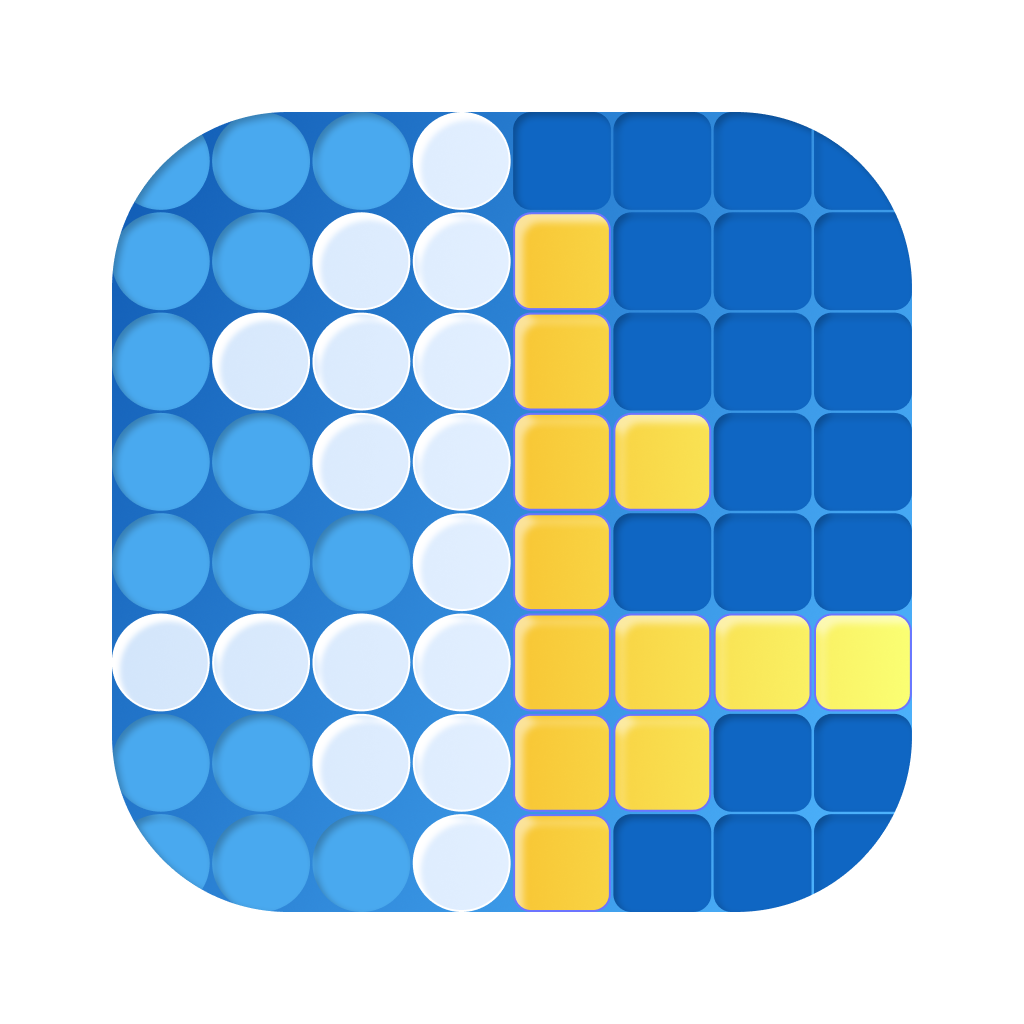
\includegraphics[width=1.5in]{figures/JarvisHEP.png}%
  \end{minipage}%
  \hspace{0.3in}%
  \begin{minipage}[c]{\dimexpr\linewidth-2.0in\relax}%
    {\fontsize{42}{46}\selectfont\@title\par}%
    \vspace{0.14in}%
    {\fontsize{17}{21}\selectfont\itshape\booksubtitle\par}%
  \end{minipage}\par
  \vspace{0.6in}%
  {\fontsize{13}{15}\selectfont\textsf{\smallcaps{\@date}}\par}
  \vfill
  {\fontsize{13}{15}\selectfont\textit{\@publisher}\par}
  \thispagestyle{empty}%
  \endgroup
}
\makeatother

%%
% Compact table of contents (tufte's default leaves a lot of vertical air between
% entries; we tighten part/chapter spacing so the chapters-only ToC stays short).
\titlecontents{part}[0pt]%
  {\addvspace{0.9\baselineskip}\large\sffamily\bfseries}%
  {\allcaps{Part~\thecontentslabel}\quad}{\allcaps{}}%
  {}[\vspace{0.15\baselineskip}]
\titlecontents{chapter}[2.6em]%
  {\itshape}%
  {\contentslabel{2.4em}}{}%
  {\qquad\normalfont\thecontentspage}[\vspace{0.12\baselineskip}]

%%
% Number chapters (tufte-book leaves them unnumbered by default).  secnumdepth=0
% numbers chapters but not sections.
\setcounter{secnumdepth}{0}

%%
% Restore a recto start (with blank-page separation) for PART dividers, while
% `openany' keeps chapters from inserting blank pages between themselves.
\let\jorigpart\part
\renewcommand{\part}{\cleardoublepage\jorigpart}

% --- Compile a subset while drafting (uncomment + edit) -----------------------
% \includeonly{chapters/01-introduction}

\begin{document}

%==============================================================================
% FRONT MATTER
%==============================================================================
\frontmatter

\maketitle

% Copyright page
\newpage
\begin{fullwidth}
~\vfill
\thispagestyle{empty}
\setlength{\parindent}{0pt}
\setlength{\parskip}{\baselineskip}
\noindent Copyright \copyright\ \the\year\ The Jarvis-HEP Developers.

\par This manual tracks \Jarvis\ and is revised with each release. This build documents
\Jarvis\ \Jversion.

\par\smallcaps{Released under the MIT License.}  Jarvis-HEP and this manual are
distributed in the hope that they will be useful, but \smallcaps{without any
warranty}; without even the implied warranty of merchantability or fitness for a
particular purpose.

\par Project home: \url{https://github.com/Pengxuan-Zhu-Phys/Jarvis-HEP}.
\par Online docs: \url{https://pengxuan-zhu-phys.github.io/Jarvis-Docs/}.

\par\textit{Manual generated \today.}
\end{fullwidth}

% Contents and lists
\tableofcontents
\listoffigures
\listoftables

% Preface
\cleardoublepage
\chapter*{Preface}
\addcontentsline{toc}{chapter}{Preface}
\markboth{Preface}{Preface}

\newthought{This manual} is the complete, ground-up reference for \Jarvis---a
\textsc{yaml}-driven framework for orchestrating likelihood-based parameter scans in
high-energy physics. It is a living document, revised in step with each \Jarvis\ release;
this build documents \Jversion. It is written for the physicist who wants to go from an empty
directory to a finished, reproducible scan, and who then wants to understand every knob
along the way.

\section*{Who this is for}

You will get the most from this book if you are comfortable running commands in a Unix
shell and editing \textsc{yaml} files. No prior experience with \Jarvis\ is assumed.
Part~\ref{part:getting-started} takes a newcomer end to end; the later parts are a
reference you can dip into key by key.

\section*{How to read it}

\begin{itemize}
  \item \textbf{New users} should read Part~\ref{part:getting-started}
        (\nameref{part:getting-started}) in order, run the quick-start scan, then skim
        Part~\ref{part:task-card} to understand the task card.
  \item \textbf{Writing a real scan?} Live in Part~\ref{part:task-card}
        (the \textsc{yaml} reference) and Part~\ref{part:backends} (calculators, operas,
        and library dependencies).
  \item \textbf{Choosing or tuning a sampler?} Part~\ref{part:samplers} has one focused
        section per method, plus a decision guide and a master comparison table.
  \item \textbf{Running, monitoring, and post-processing?} Part~\ref{part:running}.
  \item \textbf{Squeezing out performance?} Part~\ref{part:advanced}.
  \item The \textbf{appendices} are lookup tables: every \textsc{cli} flag, every
        \textsc{yaml} key, every distribution, every sampler.
\end{itemize}

\section*{Conventions}

\begin{description}[style=nextline, leftmargin=1.2em]
  \item[\code{monospace}] Code, file names, \textsc{yaml} keys, and shell commands.
  \item[\marker{\&J/}] The path \emph{marker} that Jarvis expands at runtime
        (Chapter~\ref{ch:core-concepts}).
  \item[\token{@SampleID}, \token{@Sdir}, \token{@PackID}] Runtime \emph{tokens} substituted
        per sample.
\end{description}

\noindent Three kinds of call-outs appear throughout:

\begin{jnote}
A clarification or a detail that is easy to miss.
\end{jnote}

\begin{jtip}
A recommended practice that will save you time.
\end{jtip}

\begin{jwarn}
A foot-gun. For example: the calculator key is spelled \yamlkey{make\_paraller}
(legacy spelling, kept on purpose), and a task card uses \emph{either} \yamlkey{Calculators}
\emph{or} \yamlkey{Operas} as its workflow backend---not both.
\end{jwarn}

\section*{What's new in this build}

As of \Jversion, \Jarvis\ ships an optional high-throughput runtime, configured entirely through the
\yamlkey{Runtime} task-card block (Chapter~\ref{ch:runtime-block}). Scans can be proposed and
persisted in batches (\yamlkey{batch\_size}), run across multiple worker processes
(\yamlkey{mode: process}, \yamlkey{Operas}-only for now), and persist through a separate writer
process (\yamlkey{writer: process}); per-sample folders are now created lazily
(\yamlkey{sample\_artifacts: auto}), with failed points still guaranteed a complete log. None of this
changes existing task cards, the \textsc{cli}, the output layout, or checkpoint behaviour---with no
\yamlkey{Runtime} block the engine runs exactly as before. Measure any of it reproducibly with
\cli{-{}-benchmark} (Chapter~\ref{ch:performance}).

\section*{Source of truth}

\Jarvis\ evolves quickly. Where this manual and the running code ever disagree, the code
wins; please report the gap on the issue tracker. Every \textsc{yaml} key printed here was
checked against the runtime configuration loader and the per-sampler \textsc{json} schemas
shipped in \schemaref{}.

\vspace{1\baselineskip}
\noindent If \Jarvis\ saves you a week of bookkeeping, it has done its job.


%==============================================================================
% MAIN MATTER
%==============================================================================
\mainmatter
% Show the chapter number + title in the running head (recto). \mainmatter sets
% \chaptermark, so we override it here to include the number.
\renewcommand{\chaptermark}[1]{\markboth{\thechapter.\ #1}{}}

\part{Getting Started}\label{part:getting-started}
\chapter{Introduction}
\label{ch:introduction}

\newthought{Jarvis-HEP is a Python framework} for orchestrating likelihood-based
parameter scans in high-energy physics.\sidenote{\Jarvis\ stands for \emph{Just a Really
Viable Interface to Suite for High Energy Physics}.} It coordinates expensive external
calculators, explores difficult parameter spaces with a large family of sampling
algorithms, persists structured outputs in \textsc{hdf5} and \textsc{csv}, and closes every
run with explicit diagnostics. You describe \emph{what} to scan in a single \textsc{yaml}
task card; \Jarvis\ handles the \emph{how}.

This chapter sets the mental model for the rest of the book: what \Jarvis\ is, the problems
it is built to solve, how a run flows internally, and where it sits among its sibling tools
\Operas\ and \JPlot.

\section{What Jarvis-HEP does}
\label{sec:what-it-does}

Parameter scans in particle physics share a recurring, tedious shape. For each point in a
parameter space you must launch one or more external programs, feed them correctly formatted
input, wait, parse their output, turn that output into a likelihood, and record everything in
a way you can analyse later and reproduce months afterward. Doing this by hand is slow and
error-prone; doing it at the scale of millions of points is impossible without
infrastructure.\cite{Guo:2026kfy}

\Jarvis\ \emph{is} that infrastructure. It keeps a set of normally separate concerns inside
one runtime:

\begin{itemize}
  \item \textbf{Sampling} --- how parameter points are drawn (random, space-filling, nested,
        \textsc{mcmc}, gradient-based, \textsc{ml}-guided, \ldots).
  \item \textbf{Workflow orchestration} --- running external calculators in dependency order,
        or evaluating in-process operators.
  \item \textbf{Likelihood evaluation} --- turning observables into a \yamlkey{LogLikelihood}.
  \item \textbf{Persistence} --- structured, post-processable \textsc{hdf5}/\textsc{csv} output.
  \item \textbf{Operability} --- logging, checkpoint/resume, monitoring, and end-of-run summaries.
\end{itemize}

\begin{jnote}
This manual is a living document, revised in step with each \Jarvis\ release; this build
documents \Jversion. \Jarvis\ runs on \textbf{Python 3.10 and newer}---every release is
validated by an automated test suite across the supported 3.10+ interpreters before it
ships, which is what ``3.10+'' means here---and is distributed under the \textsc{mit} License.
\end{jnote}

\section{The three-step mental model}
\label{sec:mental-model}

Everything in \Jarvis\ is organised around a single idea. For every parameter point, a run
does exactly three things:

\begin{enumerate}
  \item \textbf{Draw a parameter point.} A \emph{sampler} proposes a point in the parameter
        space you defined under \yamlkey{Sampling.Variables}.
  \item \textbf{Run a workflow that turns that point into observables.} Either external
        \yamlkey{Calculators} (file-based programs) or in-process \yamlkey{Operas}
        (Python operators) consume the point and produce named observables.
  \item \textbf{Compute a \yamlkey{LogLikelihood} from those observables.} One or more named
        expressions score the point; the sampler uses that score to decide what to do next.
\end{enumerate}

\begin{marginfigure}
\centering
\smallcaps{point}\\[2pt]
$\big\downarrow$ \emph{sampler}\\[2pt]
\smallcaps{workflow}\\[2pt]
$\big\downarrow$ \emph{calculators / operas}\\[2pt]
\smallcaps{observables}\\[2pt]
$\big\downarrow$ \emph{LogLikelihood}\\[2pt]
\smallcaps{score}
\caption[The per-point loop.]{The per-point loop. Keep this picture in mind; every task card
is a way to fill in these three arrows.}
\label{fig:per-point-loop}
\end{marginfigure}

Hold on to Figure~\ref{fig:per-point-loop}. A \Jarvis\ task card is nothing more than a
precise way of filling in those three steps, plus the bookkeeping around them. The whole of
Part~\ref{part:task-card} is a field-by-field tour of that card.

\section{Problems it is built to solve}
\label{sec:problems}

\Jarvis\ targets scan workflows that are painful to manage by hand: expensive external
calculators, sparse or fine-tuned parameter regions, profile-likelihood style studies, and
output bookkeeping that has to stay reproducible. Table~\ref{tab:at-a-glance} maps those pain
points to the framework's answers.

\begin{table}[ht]
  \footnotesize
  \begin{tabular}{@{}p{0.42\linewidth}p{0.5\linewidth}@{}}
    \toprule
    \textbf{Problem} & \textbf{Jarvis-HEP answer} \\
    \midrule
    External program orchestration & Ordered calculator workflow with async-friendly execution \\
    Hard-to-scan parameter spaces & Many sampler families: random and Bridson through nested and \textsc{mcmc} \\
    Output sprawl & Project-local outputs, logs, images, and packaged rerun workflows \\
    Post-run analysis & \textsc{hdf5} storage plus schema-driven \textsc{csv} conversion \\
    Run visibility & Logger-routed diagnostics and end-of-run summaries \\
    \bottomrule
  \end{tabular}
  \caption{What \Jarvis\ is for, at a glance.}
  \label{tab:at-a-glance}
\end{table}

\section{Design principles}
\label{sec:principles}

A handful of decisions shape how the framework feels in daily use. They are worth stating up
front, because they explain many of the defaults you will meet later.

\begin{description}[style=nextline, leftmargin=1.2em]
  \item[No repo-root requirement] Normal usage runs from a \emph{standalone project}
        directory, not from a checkout of the framework. Chapter~\ref{ch:core-concepts}
        explains the project markers.
  \item[Project-local outputs by default] Every run writes under your project root, so a
        scan is self-contained and easy to move or archive.
  \item[Explicit logging over silent failure] When something goes wrong, \Jarvis\ tells you,
        and a failed sample can replay its buffered log for forensic analysis.
  \item[Structured, post-processable outputs] Results land in \textsc{hdf5} with schema and
        \textsc{csv} export, so they remain usable long after the run ends.
  \item[Additive diagnostics] Run summaries and monitoring are built in, not bolted on.
\end{description}

\section{How a run flows}
\label{sec:run-flow}

Internally, a scan threads through a fixed pipeline. You do not need to memorise it to use
\Jarvis, but seeing it once makes the later chapters click into place:

\begin{quote}
\sffamily\footnotesize
Task \textsc{yaml} $\rightarrow$ Sampler $\rightarrow$ Factory / Workflow $\rightarrow$
Calculator or Opera modules $\rightarrow$ Structured outputs $+$ Logs \& run summary
\end{quote}

The command-line entry point loads and validates your task card, instantiates the sampler
you named, builds the calculator/opera dependency graph, spins up a worker pool, runs the
per-point loop of Section~\ref{sec:mental-model}, streams results into the \textsc{hdf5}
writer, and finishes with a machine- and human-readable summary. Inside a calculator module,
the maintained execution order is always the same---\emph{write input files, run external
commands, read output files}---a contract we return to in Chapter~\ref{ch:calculators}.

\section{What you will produce}
\label{sec:what-you-produce}

A finished run leaves a predictable set of project-local artifacts. You will meet each in
detail in Part~\ref{part:running}; for now, a preview:

\begin{itemize}
  \item \file{outputs/<scan>/DATABASE/} --- \textsc{hdf5} samples, schema files, \textsc{csv}
        exports, and run metadata.
  \item \file{outputs/<scan>/SAMPLE/} --- per-sample working files and retained artifacts.
  \item \file{logs/<scan>/} --- Jarvis, sampler, and runtime logs.
  \item \file{images/<scan>/} --- the semantic \file{flowchart.json}, generated plot configs,
        and figures.
  \item \file{run\_summary.json}, \file{run\_summary.csv}, \file{run\_summary.txt} ---
        end-of-run summaries.
\end{itemize}

\section{The Jarvis ecosystem}
\label{sec:ecosystem}

\Jarvis\ ships alongside two sibling projects. You can use \Jarvis\ on its own, but together
they cover the full scan-to-figure path (Table~\ref{tab:ecosystem}).

\begin{table}[ht]
  \footnotesize
  \begin{tabular}{@{}lp{0.62\linewidth}@{}}
    \toprule
    \textbf{Project} & \textbf{Role} \\
    \midrule
    \Jarvis  & Sampling, workflow orchestration, persistence (this manual). \\
    \Operas  & In-process operator library for \yamlkey{Operas} workflows; installed by
               default and used by the built-in quick-starts (Chapter~\ref{ch:jarvis-operas}). \\
    \JPlot   & Plotting and flowchart rendering from \Jarvis\ outputs; optional
               (Chapter~\ref{ch:jarvisplot}). \\
    \bottomrule
  \end{tabular}
  \caption{The three Jarvis projects.}
  \label{tab:ecosystem}
\end{table}

\section{Where to go next}
\label{sec:next}

\begin{itemize}
  \item If you have not installed \Jarvis\ yet, go to Chapter~\ref{ch:installation}.
  \item To run something immediately, jump to the quick start in
        Chapter~\ref{ch:quickstart}.
  \item To understand the vocabulary used throughout the book---projects, path markers, and
        runtime tokens---read Chapter~\ref{ch:core-concepts}.
\end{itemize}

\begin{jtip}
If you remember only one thing from this chapter, make it the three-step loop of
Figure~\ref{fig:per-point-loop}. Every feature in this manual hangs off one of those three
arrows.
\end{jtip}

\chapter{Installation}
\label{ch:installation}

\newthought{Getting \Jarvis\ onto your machine} takes a single \cli{pip} command. This
chapter covers the quick install, the optional extras, how to verify the result, and how to
keep \Jarvis\ in a clean, isolated environment so it never collides with your other Python
work.

\section{What you install}
\label{sec:what-you-install}

\Jarvis\ is distributed on \textsc{PyPI} as a small ecosystem of Python packages
(Table~\ref{tab:packages}). The core package, \code{Jarvis-HEP}, is the only one you must
install explicitly; it pulls in \Operas\ automatically because the built-in quick-starts use
it.

\begin{table}[ht]
  \footnotesize
  \begin{tabular}{@{}lll@{}}
    \toprule
    \textbf{Package} & \textbf{Provides} & \textbf{How it arrives} \\
    \midrule
    \code{Jarvis-HEP}        & core runner, samplers, \textsc{cli} (\cmd{Jarvis}) & you install it \\
    \code{Jarvis-Operas}     & in-process operators (\cmd{jopera})               & pulled in automatically \\
    \code{Jarvis-HEP-Portal} & supporting runtime services                       & pulled in automatically \\
    \code{JarvisPLOT}        & plotting \& flowchart rendering (\cmd{jplot})      & optional, install separately \\
    \bottomrule
  \end{tabular}
  \caption{The \Jarvis\ package ecosystem on \textsc{PyPI}.}
  \label{tab:packages}
\end{table}

\begin{jnote}
Most users never need a \textsc{git} checkout of the framework. Install from \textsc{PyPI}
and work inside a standalone \emph{project} directory (Chapter~\ref{ch:core-concepts}).
\end{jnote}

\section{Requirements}
\label{sec:requirements}

\Jarvis\ runs on \textbf{Python 3.10 and newer}, on Linux and macOS. The ``3.10+'' is a
\emph{supported, continuously-tested range}, not an arbitrary floor: before every release the
test suite runs automatically across the supported 3.10+ interpreters, so any version in that
range is one we have actually validated.\sidenote{If you must use an older Python, \Jarvis\
will not install---upgrade the interpreter or create a dedicated 3.10+ environment as in
Section~\ref{sec:clean-env}.}

\begin{jtip}
Install into a \emph{clean virtual environment}. It keeps \Jarvis's dependency set (NumPy,
SciPy, h5py, PyTorch, and friends) from clashing with other projects, and makes the whole
thing trivial to remove later.
\end{jtip}

\section{Quick install}
\label{sec:quick-install}

For most users, one command is enough:

\begin{shellbox}
python3 -m pip install -U Jarvis-HEP
\end{shellbox}

\noindent The \cli{-U} flag upgrades \Jarvis\ and its dependencies to the latest compatible
versions. This installs the \cmd{Jarvis} executable as a console entry point on your
\code{PATH} (Section~\ref{sec:verify} shows how to confirm where it landed).

\section{Optional extras}
\label{sec:extras}

Beyond the core package, two optional pieces are commonly added: the plotting sibling
package, and any external backends that a particular sampler or calculator needs.

\paragraph{Plotting} lives in the separate \code{JarvisPLOT} package, which provides the
\cmd{jplot} command and is what \cli{Jarvis ... -{}-plot} hands off to
(Chapter~\ref{ch:jarvisplot}):

\begin{shellbox}
python3 -m pip install -U JarvisPLOT
\end{shellbox}

\paragraph{External backends} such as \textsc{MultiNest}, \textsc{Diver}, or CERN
\textsc{root} are independent native programs. Install them following their own
instructions; \Jarvis\ detects and drives them when your task card asks for them. A few
optional Python-based samplers likewise depend on extra packages. In every case the relevant
sampler chapter in Part~\ref{part:samplers} states the exact prerequisite and how to install
it, so you only ever add what your scan actually uses.

\begin{jnote}
A full ``everything'' install is simply the three \textsc{PyPI} packages together:
\begin{shellbox}
python3 -m pip install -U Jarvis-HEP Jarvis-Operas JarvisPLOT
\end{shellbox}
After it you will have the \cmd{Jarvis}, \cmd{jopera}, and \cmd{jplot} commands.
\end{jnote}

\section{A clean environment (recommended)}
\label{sec:clean-env}

Any environment manager works---\code{venv}, \code{conda}, \code{uv}, or \code{pyenv}---as
long as it gives you an isolated 3.10+ interpreter. A \code{pyenv}~+~\code{virtualenv}
recipe:

\begin{shellbox}
pyenv install 3.10.12
pyenv virtualenv 3.10.12 jarvis-hep
pyenv activate jarvis-hep
python3 -m pip install -U Jarvis-HEP
\end{shellbox}

\noindent The plain-\code{venv} equivalent:

\begin{shellbox}
python3 -m venv ~/.venvs/jarvis-hep
source ~/.venvs/jarvis-hep/bin/activate
python3 -m pip install -U Jarvis-HEP
\end{shellbox}

\section{Verifying the install}
\label{sec:verify}

Two commands confirm everything is in place:

\begin{shellbox}
Jarvis --version
Jarvis --help
\end{shellbox}

\noindent \cli{Jarvis -{}-version} prints the \Jarvis\ banner and the runtime version of the
installed package (Figure~\ref{fig:version-banner})---a quick way to check exactly which
release you are running. The coloured dot-matrix on the left is the \Jarvis\ icon; the wordmark
fades from blue to gold, and the final line carries the live version of \emph{your} install.

\begin{figure}[ht]
\centering
\JarvisVersionBanner
\caption[The \cli{Jarvis -{}-version} banner.]{The \cli{Jarvis -{}-version} banner, reproduced
in the project's own palette. The version on the last line is read from your installed package
at runtime; here it shows the release this manual documents.}
\label{fig:version-banner}
\end{figure}

\noindent \cli{Jarvis -{}-help} prints the two entry points (a \textsc{yaml} file, or a
\cli{project} subcommand) and the available options; the full \textsc{cli} is documented in
Chapter~\ref{ch:cli}.

\begin{jwarn}
If your shell reports \cli{Jarvis: command not found}, the executable is not on your
\code{PATH}---almost always because you installed into a different environment than the one
you are using now. Re-activate the environment where you ran \cli{pip install}, and confirm
with \cli{which Jarvis}. Under \code{pyenv}, \cmd{Jarvis} lives in that version's \code{bin/}
directory.
\end{jwarn}

\section{Where to go next}
\label{sec:install-next}

With \Jarvis\ installed and verified, head to Chapter~\ref{ch:quickstart} to create a project
and run your first scan in a couple of minutes.

\chapter{Your First Scan}
\label{ch:quickstart}

\newthought{The fastest way to understand \Jarvis} is to run it. This chapter takes you from
an empty directory to a finished scan with structured output, using the quick-start cards
that ship inside every new project. You will not write any \textsc{yaml} yet---that comes in
Part~\ref{part:task-card}---you will just run, watch, and read the results.

\section{Create a project}
\label{sec:create-project}

\Jarvis\ works inside a \emph{standalone project}: a self-contained directory that holds your
task cards and collects all outputs. Create one with:

\begin{shellbox}
Jarvis project create MyScan
cd MyScan
\end{shellbox}

\noindent This scaffolds a ready-to-run project:

\begin{jfiletree}
\dirtree{%
.1 \dtfold{MyScan/}.
.2 \dtfold{bin/}.
.3 \dtcode{quickstart\_mcmc\_operas.yaml}.
.3 \dtcode{quickstart\_csv\_operas.yaml}.
.2 \dtfold{data/}.
.3 \dtcsv{points.csv}.
.2 \dtfold{deps/}.
.3 \dtcode{environment\_default.yaml}.
.2 \dtdoc{README.md}.
.2 \dtmark{.jarvis-project.json}\DTcomment{project marker}.
.2 \dtyaml{jarvis.project.yaml}\DTcomment{project marker}.
}
\end{jfiletree}

\begin{description}[style=nextline, leftmargin=1.2em]
  \item[\dtfold{bin/}] Your \textsc{yaml} task cards live here; two quick-starts are provided.
  \item[\dtfold{data/}] External data files (here, a small \file{points.csv} for the replay
        example).
  \item[\dtfold{deps/}] Dependency declarations, including a default environment file.
  \item[\dtmark{.jarvis-project.json}, \dtyaml{jarvis.project.yaml}] \emph{Marker files} that tell
        \Jarvis\ ``this directory is the project root.'' They are what the \marker{\&J/} path
        marker resolves to (Chapter~\ref{ch:core-concepts}).
\end{description}

\begin{jnote}
Runtime directories---\file{outputs/}, \file{logs/}, and \file{images/}---are \emph{not}
created up front. \Jarvis\ makes them on first use, so a fresh project stays tidy.
\end{jnote}

\section{The quick-start card at a glance}
\label{sec:quickstart-card}

Open \file{bin/quickstart\_mcmc\_operas.yaml}. It is a complete, minimal task card
(shown below). Do not worry about every key yet---just match it to the
three-step mental model from Chapter~\ref{ch:introduction}.

\begin{yamlwin}[bin/quickstart\_mcmc\_operas.yaml]
Scan:
  name: "quickstart_mcmc_operas"
  save_dir: "&J/outputs"
  sample_directory:
    limit: 200
    width: 6
    archive_samples: true

Sampling:
  Method: "MCMC"
  Variables:
    - name: x
      description: "Toy variable x"
      distribution: {type: Flat, parameters: {min: 0, max: 5.0}}
    - name: y
      description: "Toy variable y"
      distribution: {type: Flat, parameters: {min: 0, max: 5.0}}
  Bounds:
    num_chains: 8
    num_iters: 600
    proposal_scale: 0.06
  LogLikelihood:
    - {name: "LogL_Z", expression: "LogGauss(z, 100, 10)"}

Operas:
  make_paraller: 8
  Modules:
    - name: EggBox
      operator: "helper.eggbox2d"
      call_mode: call
      required_modules: []
      input:
        - {name: x, expression: "x"}
        - {name: y, expression: "y"}
      output:
        - {name: z, entry: z}
\end{yamlwin}

\noindent Reading it against the three steps:

\begin{enumerate}
  \item \textbf{Draw a point.} \yamlkey{Sampling} runs the \sampler{MCMC} sampler over two
        flat variables \yamlkey{x} and \yamlkey{y} on $[0, 5]$.
  \item \textbf{Run a workflow.} \yamlkey{Operas} evaluates the in-process operator
        \code{helper.eggbox2d} on \yamlkey{x} and \yamlkey{y} and produces the observable
        \yamlkey{z}.
  \item \textbf{Score it.} \yamlkey{LogLikelihood} computes \expr{LogGauss(z, 100, 10)}---a
        Gaussian centred on a pretend measurement $z = 100 \pm 10$.
\end{enumerate}

\noindent The \yamlkey{Scan} block names the run and points outputs at \marker{\&J/outputs}.
(The card also declares an \yamlkey{EnvReqs} block, omitted from the listing for brevity, that
checks the platform before starting.)

\section{Run it}
\label{sec:run-it}

From the project root:

\begin{shellbox}
Jarvis bin/quickstart_mcmc_operas.yaml
\end{shellbox}

\noindent You will see, in order:

\begin{enumerate}
  \item the \Jarvis\ banner and version---the logging system is up;
  \item \code{Validation successful}---your card passed the schema check;
  \item the sampler initialising (here, \sampler{MCMC});
  \item the worker factory building and the workflow flowchart being drawn;
  \item periodic progress lines as samples are submitted and completed;
  \item an end-of-run summary from the \textsc{hdf5} writer and the factory, followed by an
        automatic conversion of the results to \textsc{csv}.
\end{enumerate}

\begin{jtip}
The terminal shows only the high-level status of the sampler and the factory. You do not need
to read it closely---everything important is captured in the project's \file{logs/} directory
and the end-of-run summary.
\end{jtip}

\section{Replay tabulated points}
\label{sec:replay}

Sometimes you already have the parameter points and just want to push them through the
workflow. The second quick-start does exactly that, reading rows from
\file{data/points.csv} instead of sampling:

\begin{shellbox}
Jarvis bin/quickstart_csv_operas.yaml
\end{shellbox}

\noindent Its only difference from the quick-start card above is the \yamlkey{Sampling}
block, which selects the \sampler{CSV} method and names the file and columns to replay:

\begin{yamlwin}
Sampling:
  Method: "CSV"
  CSV:
    path: "&J/data/points.csv"
    uuid_column: "uuid"
    variables: ["x", "y"]
  LogLikelihood:
    - {name: "LogL_Z", expression: "LogGauss(z, 100, 10)"}
\end{yamlwin}

\section{Look at what you produced}
\label{sec:first-outputs}

After either run, your project has gained a predictable set of artifacts under the run name:

\begin{jfiletree}
\dirtree{%
.1 \dtfold{MyScan/}.
.2 \dtfold{outputs/quickstart\_mcmc\_operas/}.
.3 \dtfold{DATABASE/}.
.4 \dtdata{samples.0.hdf5}\DTcomment{structured samples}.
.4 \dtcsv{samples.0.csv}\DTcomment{CSV export}.
.4 \dtcode{samples.schema.json}\DTcomment{observable schema}.
.3 \dtfold{SAMPLE/}\DTcomment{per-sample artifacts}.
.3 \dtcode{run\_summary.\{json,csv,txt\}}\DTcomment{run summaries}.
.2 \dtfold{logs/quickstart\_mcmc\_operas/}\DTcomment{run logs}.
.2 \dtfold{images/quickstart\_mcmc\_operas/}\DTcomment{flowchart.json, plots}.
}
\end{jfiletree}

\noindent The \file{DATABASE/} folder is what you analyse: \textsc{hdf5} for tools, \textsc{csv}
for a quick look, and a schema describing the columns. The \file{run\_summary.*} files report
how the run went. All of this is covered in detail in Part~\ref{part:running}.

\section{Convert, plot, and monitor}
\label{sec:quickstart-utilities}

Three optional commands operate on a run; each is detailed in Chapter~\ref{ch:cli}:

\begin{description}[style=nextline, leftmargin=1.2em]
  \item[\cli{Jarvis bin/quickstart\_mcmc\_operas.yaml -{}-convert}] Snapshot the live
        \textsc{hdf5} into \textsc{csv} while the scan is still running.
  \item[\cli{Jarvis bin/quickstart\_mcmc\_operas.yaml -{}-plot}] Generate a \JPlot\
        configuration from the task card (then render it with \cmd{jplot}).
  \item[\cli{Jarvis bin/quickstart\_mcmc\_operas.yaml -{}-monitor}] Open a real-time resource
        monitor for a running scan.
\end{description}

\section{The success checklist}
\label{sec:success-check}

Your first scan worked if all of the following are true:

\begin{itemize}
  \item the command exited without an error;
  \item \file{outputs/<run>/DATABASE/} contains a \file{.hdf5} and a \file{.csv};
  \item \file{run\_summary.txt} reports completed samples and zero (or few) failures.
\end{itemize}

\section{Make it your own}
\label{sec:make-your-own}

You now have the full loop working end to end. The natural next steps:

\begin{itemize}
  \item Learn the vocabulary---projects, markers, tokens, and the output
        contract---in Chapter~\ref{ch:core-concepts}.
  \item Understand every block of the task card in Part~\ref{part:task-card}.
  \item Wrap your own external program as a calculator in Chapter~\ref{ch:calculators}, using
        the same black-box pattern the quick-starts follow.
\end{itemize}

\chapter{Core Concepts}
\label{ch:core-concepts}

\newthought{A handful of ideas} recur on every page of this manual: the task card, the
standalone project, the path markers and runtime tokens that make paths portable, and the
fixed contract for where output lands. Understand these five and the rest of the book is
detail. None of them require code---they are conventions \Jarvis\ enforces so that scans stay
self-contained and reproducible.

\section{The task card}
\label{sec:task-card}

A \emph{task card} is a single \textsc{yaml} file that fully describes one scan. It is the only
thing you normally edit. As Chapter~\ref{ch:introduction} put it, every card fills in the same
three steps for each parameter point: draw a point, run a workflow to get observables, and
score them with a \yamlkey{LogLikelihood}.

A card is organised into a small set of top-level blocks. You will meet each in detail in
Part~\ref{part:task-card}; the shape is:

\begin{yamlwin}
Scan:         # run name + where outputs go
Sampling:     # how points are drawn + the objective
Calculators:  # external-program workflow   (choose one backend)
Operas:       # in-process workflow         (choose one backend)
EnvReqs:      # platform + dependency contract
LibDeps:      # shared external libraries (optional)
Utils:        # helper functions (optional)
\end{yamlwin}

\noindent \yamlkey{Scan} and \yamlkey{Sampling} are required; \yamlkey{EnvReqs} is strongly
recommended; the rest are optional, with one important rule covered in
Section~\ref{sec:backends}.

\section{Standalone projects}
\label{sec:standalone-projects}

\Jarvis\ deliberately has \emph{no repo-root requirement}. You do not run it from a checkout of
the framework; you run it from \emph{your} project directory. A project is just a folder
containing two \emph{marker files}:

\begin{description}[style=nextline, leftmargin=1.2em]
  \item[\file{.jarvis-project.json}] machine-readable project metadata;
  \item[\file{jarvis.project.yaml}] human-editable project metadata.
\end{description}

\noindent When \Jarvis\ starts, it walks upward from your task card looking for either marker
and treats the directory that holds it as the \emph{task root}. Everything project-local is
resolved relative to that root. \cli{Jarvis project create} (Chapter~\ref{ch:quickstart})
writes both markers for you.

\begin{jnote}
You can override the task root explicitly by setting the environment variable
\code{JARVIS\_HEP\_TASK\_ROOT} (or \code{JHEP\_TASK\_ROOT}). If no marker is found and no
override is set, \Jarvis\ falls back to the current working directory. Setting the markers is
the robust, recommended way.
\end{jnote}

\section{Path markers}
\label{sec:path-markers}

Hard-coded absolute paths make a project impossible to move or share. \Jarvis\ solves this with
a \emph{path marker}: a short symbol that expands to a real directory at runtime.

The one public path marker is \marker{\&J}:

\begin{table}[ht]
  \footnotesize
  \begin{tabular}{@{}ll@{}}
    \toprule
    \textbf{Marker} & \textbf{Expands to} \\
    \midrule
    \marker{\&J/...} & the standalone project root (the task root of
                       Section~\ref{sec:standalone-projects}) \\
    \bottomrule
  \end{tabular}
  \caption[The public path marker.]{The public path marker. Always write project-local paths
           with \marker{\&J/}.}
  \label{tab:markers}
\end{table}

\noindent So \marker{\&J/outputs} means ``the \file{outputs/} directory inside this project,''
wherever the project happens to live. Because the marker is resolved fresh on every run, the
same card works on your laptop, a collaborator's machine, or an \textsc{hpc} node with no
edits.

\begin{jnote}
\marker{\&J/} is the only path marker you need. Keep everything a scan depends on inside the
project and reference it with \marker{\&J/...}; for a shared default file, keep a copy under
\marker{\&J/deps/...} and point to that---exactly what the built-in quick-starts do.
\end{jnote}

\section{Runtime tokens}
\label{sec:runtime-tokens}

Where a path marker names a \emph{directory}, a \emph{runtime token} names a value that changes
\emph{per sample}. Tokens let one calculator definition give every sample its own isolated
working directory and file names. There are three (Table~\ref{tab:tokens}).

\begin{table}[ht]
  \footnotesize
  \begin{tabular}{@{}lp{0.62\linewidth}@{}}
    \toprule
    \textbf{Token} & \textbf{Substituted with} \\
    \midrule
    \token{@SampleID} & the current sample's \textsc{uuid} \\
    \token{@Sdir}     & the current sample's save directory, under
                        \file{outputs/.../SAMPLE/<uuid>} (or \file{.../SAMPLE/tests/<uuid>}
                        under \cli{-{}-check-modules}) \\
    \token{@PackID}   & a calculator module \emph{instance} id, enabling per-instance working
                        directories so parallel samples never clobber each other \\
    \bottomrule
  \end{tabular}
  \caption[Runtime tokens.]{Runtime tokens, substituted per sample on calculator workflow
           paths.}
  \label{tab:tokens}
\end{table}

\noindent These tokens are available on calculator workflow paths---commands, working
directories, and sample-scoped input/output file paths. You will use \token{@PackID} heavily
when wrapping external programs (Chapter~\ref{ch:calculators}); \token{@Sdir} when you want a
calculator to write into the per-sample artifact directory.

\begin{jnote}
Referencing \token{@Sdir} (or running any calculator workflow) causes \Jarvis\ to
\emph{materialize} a per-sample directory on disk. Pure-\yamlkey{Operas} scans can skip that
filesystem work entirely---a performance lever discussed in
Chapter~\ref{ch:runtime-block}.
\end{jnote}

\section{The output contract}
\label{sec:output-contract}

Every run writes a predictable tree, derived from \yamlkey{Scan.name} (written \code{<scan>}
below). Knowing this layout means you always know where to look.

\begin{table}[ht]
  \footnotesize
  \begin{tabular}{@{}p{0.45\linewidth}p{0.47\linewidth}@{}}
    \toprule
    \textbf{Location} & \textbf{Contents} \\
    \midrule
    \file{outputs/<scan>/DATABASE/} & \textsc{hdf5} samples, schema, \textsc{csv} exports, run metadata \\
    \file{outputs/<scan>/SAMPLE/}   & per-sample working files and retained artifacts \\
    \file{logs/<scan>/}             & Jarvis, sampler, and runtime logs \\
    \file{images/<scan>/}           & semantic \file{flowchart.json}, plot configs, figures \\
    \file{outputs/<scan>/run\_summary.\{json,csv,txt\}} & end-of-run summaries \\
    \bottomrule
  \end{tabular}
  \caption[The output contract.]{The project-local output contract. Every run follows it.}
  \label{tab:output-contract}
\end{table}

\noindent Two details worth remembering now:

\begin{itemize}
  \item The \file{DATABASE/} path is shared between a normal run and a \cli{-{}-check-modules}
        dry run; only the \file{SAMPLE/} side differs (the check writes under
        \file{SAMPLE/tests/}).
  \item \Jarvis\ always writes \file{flowchart.json} (a semantic description of your workflow);
        if \JPlot\ is installed it additionally renders \file{flowchart.png}. The
        \cli{-{}-skip-draw-flowchart} flag suppresses only the \textsc{png} step.
\end{itemize}

Part~\ref{part:running} returns to each of these artifacts in depth.

\section{Choosing a workflow backend}
\label{sec:backends}

The workflow---step two of the loop---is provided by \emph{one} of two backends:

\begin{description}[style=nextline, leftmargin=1.2em]
  \item[\yamlkey{Calculators}] drives external programs through files and shell commands. Use
        it for compiled \textsc{hep} packages and file-based toolchains
        (Chapter~\ref{ch:calculators}).
  \item[\yamlkey{Operas}] evaluates in-process Python operators. Use it for algebraic or
        array-based work, and for fast prototyping (Chapter~\ref{ch:operas}).
\end{description}

\begin{jwarn}
A task card uses \emph{either} \yamlkey{Calculators} \emph{or} \yamlkey{Operas} as its workflow
backend, not both. Pick the one that matches your tools; the quick-starts in
Chapter~\ref{ch:quickstart} use \yamlkey{Operas} because the \code{EggBox} toy is an in-process
operator.
\end{jwarn}

\section{Putting it together}
\label{sec:concepts-together}

With the vocabulary in hand, the whole framework reads cleanly: you author a \emph{task card}
inside a \emph{standalone project}; \marker{\&J/} keeps its paths portable and runtime tokens
isolate each sample; a sampler draws points, your chosen \emph{backend} turns them into
observables, a \yamlkey{LogLikelihood} scores them, and the results land in the fixed
\emph{output contract}. The next part dissects the task card block by block.


\part{The Task Card: YAML Reference}\label{part:task-card}
\chapter{Task YAML Structure}
\label{ch:task-yaml}

\newthought{A task card is one \textsc{yaml} file} that describes a whole scan. This chapter is
the map: it shows the handful of top-level blocks a card can contain, says which are required,
and points you to the chapter that documents each one in detail. Read it once to get the shape;
then dip into the later chapters as you write.

\section{The shape of a card}
\label{sec:card-shape}

Recall the three-step model from Chapter~\ref{ch:introduction}: for every point, \Jarvis\
\emph{draws a point}, \emph{runs a workflow} to get observables, and \emph{scores} them with a
likelihood. A task card simply fills in those steps. Here is the full skeleton---you will rarely
use every block at once:

\begin{yamlwin}
Scan:          # run name + where outputs go          (required)
Sampling:      # how points are drawn + the objective  (required)
EnvReqs:       # platform + dependency checks           (recommended)
Calculators:   # external-program workflow  )  choose
Operas:        # in-process workflow        )  ONE of these
LibDeps:       # shared external libraries             (optional)
Utils:         # helper functions for expressions      (optional)
\end{yamlwin}

\section{Required, recommended, optional}
\label{sec:required-optional}

Only two blocks are mandatory; the rest you add when you need them
(Table~\ref{tab:blocks}).

\begin{table}[ht]
  \footnotesize
  \begin{tabular}{@{}llp{0.46\linewidth}@{}}
    \toprule
    \textbf{Block} & \textbf{Status} & \textbf{What it does} \\
    \midrule
    \yamlkey{Scan}        & required    & names the run and sets the output location \\
    \yamlkey{Sampling}    & required    & chooses the sampler, the scan variables, and the likelihood \\
    \yamlkey{EnvReqs}     & recommended & checks the machine before the run starts \\
    \yamlkey{Calculators} & one backend & runs external programs to produce observables \\
    \yamlkey{Operas}      & one backend & runs in-process Python operators instead \\
    \yamlkey{LibDeps}     & optional    & installs shared external libraries once \\
    \yamlkey{Utils}       & optional    & defines helper functions used in expressions \\
    \bottomrule
  \end{tabular}
  \caption{The top-level blocks of a task card.}
  \label{tab:blocks}
\end{table}

\begin{jwarn}
Pick \emph{one} workflow backend: a card uses \yamlkey{Calculators} \emph{or} \yamlkey{Operas},
not both. Use \yamlkey{Operas} for quick, in-process calculations and \yamlkey{Calculators} to
drive external programs (Chapter~\ref{ch:core-concepts} explains the choice).
\end{jwarn}

\section{A complete minimal card}
\label{sec:minimal-card}

The quick-start from Chapter~\ref{ch:quickstart} is a real, complete card. Stripped to its
essentials it is just \yamlkey{Scan} + \yamlkey{Sampling} + a backend:

\begin{yamlwin}
Scan:
  name: "my_first_scan"
  save_dir: "&J/outputs"

Sampling:
  Method: "Random"
  Variables:
    - name: x
      distribution: {type: Flat, parameters: {min: 0, max: 5}}
  LogLikelihood:
    - {name: "LogL", expression: "-0.5 * (x - 2)**2"}

Operas:
  make_paraller: 4
  Modules: []
\end{yamlwin}

\noindent Everything else in this part of the book is about filling these blocks in with more
detail and confidence.

\section{Where each block is documented}
\label{sec:block-map}

\begin{description}[style=nextline, leftmargin=1.2em]
  \item[\yamlkey{Scan}] Chapter~\ref{ch:scan-block} --- run name, output directory, sample
        retention.
  \item[\yamlkey{Sampling}] Chapter~\ref{ch:sampling-block} (the block),
        Chapter~\ref{ch:variables} (scan variables), Chapter~\ref{ch:loglikelihood}
        (the likelihood), and Part~\ref{part:samplers} (one chapter per sampler).
  \item[\yamlkey{EnvReqs}] Chapter~\ref{ch:envreqs} --- platform and dependency checks.
  \item[\yamlkey{Calculators}] Chapter~\ref{ch:calculators} --- external-program workflows.
  \item[\yamlkey{Operas}] Chapter~\ref{ch:operas} --- in-process operator workflows.
  \item[\yamlkey{LibDeps}] Chapter~\ref{ch:libdeps} --- shared external libraries.
  \item[\yamlkey{Utils}] Chapter~\ref{ch:utils} --- helper functions for expressions.
\end{description}

\noindent Two cross-cutting topics support all of these: the \emph{expressions} you write in
likelihoods and mappings (Chapter~\ref{ch:symbols}) and the \emph{path markers and tokens}
that keep paths portable (Chapter~\ref{ch:core-concepts}).

\begin{jtip}
\textsc{yaml} is whitespace-sensitive: indent with spaces (never tabs), and keep items under a
key aligned. If \Jarvis\ reports a validation error, it almost always points at the block and
key where the indentation or a value is wrong.
\end{jtip}

\chapter{The Scan Block}
\label{ch:scan-block}

\newthought{The \yamlkey{Scan} block} answers two questions: \emph{what is this run called}, and
\emph{where do its outputs go}. It is small, but it decides the whole directory layout, so it is
worth understanding clearly.

\section{The minimal form}
\label{sec:scan-minimal}

Most cards need only two keys:

\begin{yamlwin}
Scan:
  name: "MSSM_Run"
  save_dir: "&J/outputs"
\end{yamlwin}

\begin{description}[style=nextline, leftmargin=1.2em]
  \item[\yamlkey{name}] A short, unique name for this run. It becomes the folder name that holds
        all the outputs, so prefer something filesystem-friendly (letters, digits, underscores).
  \item[\yamlkey{save\_dir}] Where output folders are created. Almost always \marker{\&J/outputs}
        --- the project-local \file{outputs/} directory. The \marker{\&J/} marker keeps the card
        portable (Chapter~\ref{ch:core-concepts}).
\end{description}

\section{What the names produce}
\label{sec:scan-layout}

\Jarvis\ builds the output tree from \yamlkey{Scan.name}. With \code{name: "MSSM\_Run"} and
\code{save\_dir: "\&J/outputs"} you get:

\begin{jfiletree}
\dirtree{%
.1 \dtfold{(project root)}.
.2 \dtfold{outputs/MSSM\_Run/}.
.3 \dtfold{DATABASE/}\DTcomment{HDF5, CSV, schema}.
.3 \dtfold{SAMPLE/}\DTcomment{per-sample files}.
.2 \dtfold{logs/MSSM\_Run/}\DTcomment{run logs}.
.2 \dtfold{images/MSSM\_Run/}\DTcomment{flowchart, plots}.
}
\end{jfiletree}

\noindent The same run name appears in \file{outputs/}, \file{logs/}, and \file{images/}, so
everything for one run is easy to find. The full output contract is described in
Chapter~\ref{ch:outputs}.

\begin{jnote}
The \file{outputs/}, \file{logs/}, and \file{images/} folders are created on first use. A fresh
project does not contain them yet.
\end{jnote}

\section{Controlling per-sample storage}
\label{sec:scan-sample-directory}

By default \Jarvis\ keeps a folder of working files for each sample under \file{SAMPLE/}. For
large scans that is a lot of folders, so the optional \yamlkey{sample\_directory} key lets you
cap and archive them:

\begin{yamlwin}
Scan:
  name: "MSSM_Run"
  save_dir: "&J/outputs"
  sample_directory:
    limit: 200
    width: 6
    archive_samples: true
\end{yamlwin}

\begin{description}[style=nextline, leftmargin=1.2em]
  \item[\yamlkey{limit}] The maximum number of live sample folders to keep at once (here, 200).
        Older ones are archived past this limit.
  \item[\yamlkey{width}] How many digits to use for the numbered folder names (here, 6, giving
        \file{000001}, \file{000002}, \ldots).
  \item[\yamlkey{archive\_samples}] When \code{true}, samples beyond the limit are compressed
        into archives instead of being kept as loose folders, keeping \file{SAMPLE/} tidy.
\end{description}

\begin{jtip}
For a quick test you can omit \yamlkey{sample\_directory} entirely. Add it once a scan grows
large enough that thousands of per-sample folders would clutter the disk. Opera-only scans can
skip per-sample folders altogether---see the \yamlkey{Runtime} options in
Chapter~\ref{ch:runtime-block}.
\end{jtip}

\section{Summary}
\label{sec:scan-summary}

\yamlkey{Scan} is two ideas: a \yamlkey{name} (which becomes the run's folder) and a
\yamlkey{save\_dir} (where that folder lives). Add \yamlkey{sample\_directory} only when you need
to control how many per-sample folders are kept. Next, the \yamlkey{Sampling} block
(Chapter~\ref{ch:sampling-block}) decides how points are drawn and scored.

\chapter{The Sampling Block}
\label{ch:sampling-block}

\newthought{The \yamlkey{Sampling} block} is the heart of a task card. It says \emph{how} points
are chosen, \emph{which} parameters vary, and \emph{how good} each point is. This chapter gives
the overall shape; the two biggest pieces---variables and the likelihood---get their own
chapters next, and each sampler is documented in Part~\ref{part:samplers}.

\section{The four parts}
\label{sec:sampling-parts}

\begin{yamlwin}
Sampling:
  Method: "Random"      # which sampler to use
  Variables: []         # the parameters to scan
  Bounds: {}            # sampler-specific settings (optional)
  LogLikelihood: []     # how to score each point
\end{yamlwin}

\begin{description}[style=nextline, leftmargin=1.2em]
  \item[\yamlkey{Method}] The name of the sampler, e.g. \sampler{Random}, \sampler{Bridson},
        \sampler{MCMC}, \sampler{Dynesty}. Choosing one is covered in
        Chapter~\ref{ch:choosing-sampler}.
  \item[\yamlkey{Variables}] The list of parameters to scan and the distribution each is drawn
        from. Full reference in Chapter~\ref{ch:variables}.
  \item[\yamlkey{Bounds}] Settings specific to the chosen \yamlkey{Method} (for example, the
        number of \textsc{mcmc} chains, or a sampler's iteration count). Each sampler's chapter
        lists its keys. Simple samplers need none.
  \item[\yamlkey{LogLikelihood}] One or more named expressions that score a point. Full
        reference in Chapter~\ref{ch:loglikelihood}.
\end{description}

\begin{jnote}
Each sampler reads its own settings from \yamlkey{Bounds} (and a few read a method-named block
such as \yamlkey{CSV} for the \sampler{CSV} replay method). Treat \yamlkey{Bounds} as ``the
dials for this sampler'' and look up the exact dials in the sampler's chapter.
\end{jnote}

\section{A worked example}
\label{sec:sampling-example}

Here is a complete \yamlkey{Sampling} block for an \sampler{MCMC} run over two variables:

\begin{yamlwin}
Sampling:
  Method: "MCMC"
  Variables:
    - name: x
      distribution: {type: Flat, parameters: {min: 0, max: 5}}
    - name: y
      distribution: {type: Flat, parameters: {min: 0, max: 5}}
  Bounds:
    num_chains: 8
    num_iters: 600
    proposal_scale: 0.06
  LogLikelihood:
    - {name: "LogL_Z", expression: "LogGauss(z, 100, 10)"}
\end{yamlwin}

\noindent Read it as a sentence: ``Run \sampler{MCMC} (with 8 chains of 600 iterations) over flat
variables \yamlkey{x} and \yamlkey{y} on $[0,5]$, scoring each point by how close the observable
\yamlkey{z} is to $100 \pm 10$.''

\section{Optional: pre-selecting points}
\label{sec:sampling-selection}

Some samplers accept an optional \yamlkey{selection}: a true/false condition that a point must
satisfy to be accepted. It is written as a symbolic expression
(Chapter~\ref{ch:symbols}):

\begin{yamlwin}
Sampling:
  selection: "(x > 0) & (y < 4)"
\end{yamlwin}

\noindent Use it to skip obviously uninteresting regions before the (often expensive) workflow
runs. The expression must evaluate to a strict boolean.

\section{Where to go next}
\label{sec:sampling-next}

\begin{itemize}
  \item To define the variables: Chapter~\ref{ch:variables}.
  \item To define the score: Chapter~\ref{ch:loglikelihood}.
  \item To choose and tune a sampler: Chapter~\ref{ch:choosing-sampler} and the per-method
        chapters in Part~\ref{part:samplers}.
\end{itemize}

\chapter{Scan Variables and Distributions}
\label{ch:variables}

\newthought{\yamlkey{Sampling.Variables}} lists the parameters you want to scan and tells \Jarvis\
how to draw values for each one. Every sampler reads the same variable format, so once you learn
it here it works everywhere.

\section{One variable at a time}
\label{sec:var-schema}

\yamlkey{Variables} is a list; each item defines \emph{one} variable:

\begin{yamlwin}
Sampling:
  Variables:
    - name: x1
      description: "A flat variable"
      distribution:
        type: Flat
        parameters:
          min: 0
          max: 10
\end{yamlwin}

\begin{description}[style=nextline, leftmargin=1.2em]
  \item[\yamlkey{name}] A short identifier, unique within the scan. You use this name later in
        likelihood and mapping expressions.
  \item[\yamlkey{description}] A one-line note on what the variable means. Optional but
        recommended---it shows up in diagnostics.
  \item[\yamlkey{distribution.type}] Which distribution to draw from (the next section lists
        them).
  \item[\yamlkey{distribution.parameters}] The numbers that distribution needs (for example
        \yamlkey{min} and \yamlkey{max}).
\end{description}

\section{The five distributions}
\label{sec:distributions}

\Jarvis\ supports the five one-dimensional distributions in Table~\ref{tab:distributions}. Each
has its own required parameters.

\begin{table}[ht]
  \footnotesize
  \begin{tabular}{@{}lll@{}}
    \toprule
    \textbf{\yamlkey{type}} & \textbf{Parameters} & \textbf{Use it when\ldots} \\
    \midrule
    \yamlkey{Flat}       & \yamlkey{min}, \yamlkey{max}        & values are equally likely across a range \\
    \yamlkey{Log}        & \yamlkey{min}, \yamlkey{max}        & the range spans orders of magnitude (\yamlkey{min}$>0$) \\
    \yamlkey{Normal}     & \yamlkey{mean}, \yamlkey{stddev}    & values cluster around a central value \\
    \yamlkey{Log-Normal} & \yamlkey{mean}, \yamlkey{stddev}    & the \emph{logarithm} clusters around a value \\
    \yamlkey{Logit}      & \yamlkey{location}, \yamlkey{scale} & a bell-like shape with heavier tails \\
    \bottomrule
  \end{tabular}
  \caption{The supported variable distributions.}
  \label{tab:distributions}
\end{table}

\paragraph{Flat (uniform)} Every value between \yamlkey{min} and \yamlkey{max} is equally likely:
$x \sim \mathcal{U}(\mathrm{min}, \mathrm{max})$. This is the default choice when you have no
prior preference.

\paragraph{Log (log-uniform)} Equally likely \emph{per decade}, so a scan covers
$10^{-3}$ as densely as $10^{3}$: $\ln x \sim \mathcal{U}(\ln\mathrm{min}, \ln\mathrm{max})$.
Requires \yamlkey{min}$>0$.

\paragraph{Normal (Gaussian)} A bell curve centred on \yamlkey{mean} with width
\yamlkey{stddev}: $x \sim \mathcal{N}(\mathrm{mean}, \mathrm{stddev})$. About 68\% of values land
within one \yamlkey{stddev} of the \yamlkey{mean}.

\paragraph{Log-Normal} A Normal distribution in $\ln x$ rather than $x$, useful for positive
quantities that vary multiplicatively: $\ln x \sim \mathcal{N}(\mathrm{mean}, \mathrm{stddev})$.

\paragraph{Logit (logistic)} A bell-like distribution with heavier tails than the Normal, set by
a centre \yamlkey{location} and width \yamlkey{scale}:
$x = \mathrm{location} + \mathrm{scale}\cdot\ln\!\big(\tfrac{u}{1-u}\big)$ for a uniform
$u \in (0,1)$, i.e. $x \sim \mathrm{Logistic}(\mathrm{location}, \mathrm{scale})$.

\begin{jwarn}
The \yamlkey{Log} distribution requires \yamlkey{min}$>0$: you cannot take the logarithm of zero
or a negative number. If part of your range must include zero or negatives, use \yamlkey{Flat}.
\end{jwarn}

\section{A multi-variable example}
\label{sec:var-example}

A scan usually mixes distributions---a flat mass here, a log-scaled coupling there:

\begin{yamlwin}
Sampling:
  Variables:
    - name: m0
      description: "Scalar mass (flat)"
      distribution: {type: Flat, parameters: {min: 100, max: 3000}}
    - name: tanb
      description: "tan(beta), log-scaled"
      distribution: {type: Log, parameters: {min: 1, max: 60}}
    - name: A0
      description: "Trilinear term (normal)"
      distribution: {type: Normal, parameters: {mean: 0, stddev: 1000}}
\end{yamlwin}

\begin{jnote}
All five distributions support \Jarvis's internal mapping from a uniform number in $[0,1]$, which
is what lets nested samplers and \textsc{mcmc} methods use them. Other families (Binomial,
Poisson, Beta, and so on) are not available as scan variables in the current version.
\end{jnote}

\section{Summary}
\label{sec:var-summary}

Each variable has a \yamlkey{name} and a \yamlkey{distribution} (a \yamlkey{type} plus its
\yamlkey{parameters}). Pick \yamlkey{Flat} for plain ranges, \yamlkey{Log} for wide positive
ranges, and the \yamlkey{Normal}/\yamlkey{Log-Normal}/\yamlkey{Logit} family when values should
concentrate around a centre. The variable names you choose here are exactly the symbols you will
use in the likelihood (Chapter~\ref{ch:loglikelihood}) and in expressions
(Chapter~\ref{ch:symbols}).

\chapter{LogLikelihood}
\label{ch:loglikelihood}

\newthought{\yamlkey{LogLikelihood}} is how a point gets a score. After the workflow turns a
parameter point into observables, \Jarvis\ evaluates these expressions to decide how good the
point is---and samplers use that score to decide what to do next.

\section{The minimal form}
\label{sec:logl-minimal}

\yamlkey{LogLikelihood} lives inside \yamlkey{Sampling} and is a list of named terms. The
simplest case is a single term:

\begin{yamlwin}
Sampling:
  LogLikelihood:
    - name: LogL
      expression: "-0.5 * chi2"
\end{yamlwin}

\begin{description}[style=nextline, leftmargin=1.2em]
  \item[\yamlkey{name}] A stable name for the term. \Jarvis\ writes its value into the sample
        record under this name, so you can inspect it afterwards.
  \item[\yamlkey{expression}] A symbolic expression (Chapter~\ref{ch:symbols}) evaluated once the
        scan variables and workflow outputs are available.
\end{description}

\begin{jnote}
Every term you list is computed and saved---even intermediate ones---so they are all available
for later analysis, not just the final score.
\end{jnote}

\section{Several terms at once}
\label{sec:logl-multi}

Real fits combine several constraints. List each as its own term so you can inspect them
separately:

\begin{yamlwin}
Sampling:
  LogLikelihood:
    - {name: "LogL_Z", expression: "LogGauss(z, 100, 10)"}
    - {name: "LogL_H", expression: "LogGauss(h, 125, 2)"}
\end{yamlwin}

\noindent Here \yamlkey{z} and \yamlkey{h} are observables produced by the workflow, and
\expr{LogGauss(value, mean, error)} is a built-in Gaussian log-likelihood
(Chapter~\ref{ch:symbols}).

\section{How the total score is formed}
\label{sec:logl-total}

The total log-likelihood is stored in the standard field \yamlkey{LogL}. There are two ways it is
set:

\paragraph{Automatic sum (default)} If you do \emph{not} define a term named \yamlkey{LogL},
\Jarvis\ adds up all your terms and stores the sum as \yamlkey{LogL}. The two-term example above
therefore produces \yamlkey{LogL\_Z}, \yamlkey{LogL\_H}, and
$\yamlkey{LogL} = \yamlkey{LogL\_Z} + \yamlkey{LogL\_H}$.

\paragraph{Explicit total} If you \emph{do} define a term named \yamlkey{LogL}, that expression
is used as the total. The other terms are still computed and saved, and your \yamlkey{LogL}
expression may reference them by name:

\begin{yamlwin}
Sampling:
  LogLikelihood:
    - {name: "LogL_Z", expression: "LogGauss(z, 100, 10)"}
    - {name: "LogL_H", expression: "LogGauss(h, 125, 2)"}
    - {name: "LogL",   expression: "LogL_Z + 0.5 * LogL_H"}
\end{yamlwin}

\noindent Use the explicit form when terms should be weighted differently, or combined in any way
other than a plain sum.

\begin{jtip}
Keep a single, clearly-named total. Downstream tools (and \JPlot) expect one \yamlkey{LogL}
column as the overall score; the named sub-terms are there for diagnostics.
\end{jtip}

\section{What an expression may use}
\label{sec:logl-inputs}

A \yamlkey{LogLikelihood} expression can reference:

\begin{itemize}
  \item scan variables from \yamlkey{Sampling.Variables} (by their \yamlkey{name});
  \item observables that the workflow (calculators or operas) produced;
  \item built-in constants and functions, and your own \yamlkey{Utils} functions
        (Chapter~\ref{ch:symbols} and Chapter~\ref{ch:utils}).
\end{itemize}

\begin{jwarn}
Every name in an expression must already exist when the term is evaluated. If a likelihood uses
an observable, make sure the module that produces it runs earlier in the workflow---otherwise the
name is undefined.
\end{jwarn}

\section{Summary}
\label{sec:logl-summary}

\yamlkey{LogLikelihood} is a list of \yamlkey{name}/\yamlkey{expression} terms. Omit a
\yamlkey{LogL} term to have \Jarvis\ sum everything automatically, or define \yamlkey{LogL}
explicitly to control the combination. Expressions read scan variables, workflow observables, and
the functions in Chapter~\ref{ch:symbols}.

\chapter{Symbolic Expressions and Markers}
\label{ch:symbols}

\newthought{Many places in a task card} take a small math \emph{expression} rather than a plain
number---likelihood terms, derived quantities, selection conditions, and input mappings. This
chapter lists the symbols you can use in those expressions, and the path markers that keep your
file paths portable.

\section{Where expressions are used}
\label{sec:expr-where}

You will write expressions in:

\begin{itemize}
  \item \yamlkey{Sampling.LogLikelihood} (Chapter~\ref{ch:loglikelihood});
  \item \yamlkey{Sampling.selection} (the accept/reject condition);
  \item calculator input actions (Chapter~\ref{ch:calculators});
  \item \yamlkey{Operas} module inputs (Chapter~\ref{ch:operas}).
\end{itemize}

\section{Built-in constants}
\label{sec:expr-constants}

Three constants are always available:

\begin{description}[style=nextline, leftmargin=1.2em]
  \item[\code{Pi}] the number $\pi$.
  \item[\code{E}] Euler's number $e$.
  \item[\code{Inf}] infinity.
\end{description}

\noindent For example, the expression \expr{x * Pi} multiplies the variable \yamlkey{x} by $\pi$.

\section{Built-in functions}
\label{sec:expr-functions}

The most useful built-ins are the likelihood helpers and the common math functions
(Table~\ref{tab:builtins}).

\begin{table}[ht]
  \footnotesize
  \begin{tabular}{@{}lp{0.56\linewidth}@{}}
    \toprule
    \textbf{Function} & \textbf{Meaning} \\
    \midrule
    \expr{LogGauss(x, mean, err)} & log of a Gaussian --- the usual likelihood term \\
    \expr{Gauss(x, mean, err)}, \expr{Normal(x, mean, err)} & the Gaussian itself \\
    \code{sqrt}, \code{log}, \code{exp} & square root, natural log, exponential \\
    \code{sin}, \code{cos}, \code{tan} & trigonometric functions \\
    \code{Abs}, \code{Min}, \code{Max} & absolute value, minimum, maximum \\
    \bottomrule
  \end{tabular}
  \caption{Common built-in functions.}
  \label{tab:builtins}
\end{table}

\noindent Hyperbolic and inverse-trigonometric functions from \code{sympy} are available too. A
typical likelihood term reads \expr{LogGauss(mh, 125.09, 3.0)}.

\section{Your own and Operas functions}
\label{sec:expr-user}

Two more sources of functions become available when you configure them:

\begin{description}[style=nextline, leftmargin=1.2em]
  \item[\yamlkey{Utils} functions] Interpolation tables and helpers you declare yourself
        (Chapter~\ref{ch:utils}). For instance a tabulated limit curve \expr{XenonSD2019(mN1)}.
  \item[\yamlkey{Operas} functions] Operators exposed through \yamlkey{Operas.Functions}, when
        \Operas\ is installed (Chapter~\ref{ch:operas}).
\end{description}

\section{What an expression can read}
\label{sec:expr-symbols}

Inside any expression you may use:

\begin{itemize}
  \item the names of your scan variables (e.g. \code{m0}, \code{tanb});
  \item observables produced by earlier workflow modules (e.g. \code{mh}, \code{Omega\_h2});
  \item the built-in constants and functions above;
  \item your \yamlkey{Utils} functions and any whitelisted \yamlkey{Operas} functions.
\end{itemize}

\begin{jwarn}
A name is only usable \emph{after} it exists. If an expression reads an observable, the module
that produces it must run earlier in the workflow.
\end{jwarn}

\section{Selection conditions}
\label{sec:expr-selection}

A \yamlkey{selection} is a true/false expression used to accept or reject a point before the
heavy work runs:

\begin{yamlwin}
Sampling:
  selection: "(M1 > 0) & (TanBETA < 50)"
\end{yamlwin}

\noindent Use \code{\&} for ``and'' and \code{|} for ``or''. The expression must evaluate to a
strict boolean (true or false).

\section{Path markers}
\label{sec:expr-markers}

Path markers are not math, but they belong to the same authoring vocabulary. The one you will use
constantly is \marker{\&J}.

\begin{description}[style=nextline, leftmargin=1.2em]
  \item[\marker{\&J}] the project (task) root. If your card is \file{PROJECT/bin/task.yaml}, then
        \marker{\&J} resolves to \file{PROJECT/}. Use it for every project-local path, e.g.
        \code{save\_dir: "\&J/outputs"} or \code{source: "\&J/deps/program"}.
\end{description}

\noindent A leading \code{\textasciitilde} is expanded to your home directory. Plain relative
paths resolve from the project root, while \code{./} and \code{../} resolve relative to the
\textsc{yaml} file's own directory.

\begin{jnote}
\marker{\&J} is the only path marker the runtime resolves. For anything a scan would otherwise
read from outside the project, keep a copy under the project (for example \marker{\&J/deps/...})
and reference that---exactly what the built-in quick-starts do.
\end{jnote}

\section{Placeholders inside commands}
\label{sec:expr-placeholders}

Calculator and library commands accept a second kind of substitution: \emph{placeholders} written
with \code{\$\{...\}}, which expand to config values in scope.

\begin{description}[style=nextline, leftmargin=1.2em]
  \item[\code{\$\{path\}}, \code{\$\{source\}}] the calculator's runtime path and source path.
  \item[\code{\$\{...\}}] any other configuration value in scope.
  \item[\token{@PackID}] a per-instance id, giving each parallel sample its own working directory
        (Chapter~\ref{ch:core-concepts}).
\end{description}

\noindent For example: \code{installation: ["cp -r \$\{source\}/* \$\{path\}"]}.

\section{Practical advice}
\label{sec:expr-advice}

\begin{itemize}
  \item Start simple and build one observable at a time.
  \item Prefer clear names over clever shorthand.
  \item If an expression depends on a module output, make sure that module runs first.
\end{itemize}

\chapter{Environment Requirements}
\label{ch:envreqs}

\newthought{The \yamlkey{EnvReqs} block} is a safety gate. It says what a scan expects from the
machine---operating system, Python version, packages---and \Jarvis\ checks all of it \emph{before}
the run starts. A failed check stops the run early with a clear message, instead of crashing
halfway through.

\section{The minimal form}
\label{sec:env-minimal}

For most users this is enough:

\begin{yamlwin}
EnvReqs:
  OS:
    - name: linux
      version: ">=5.10.0"
    - name: Darwin
      version: ">=10.14"
  Python:
    version: ">=3.10"
    Dependencies: []
\end{yamlwin}

\noindent It says ``run on Linux $\geq 5.10$ or macOS (\code{Darwin}) $\geq 10.14$, with Python
$3.10$ or newer.'' That covers a typical setup.

\section{The keys}
\label{sec:env-keys}

\paragraph{\yamlkey{OS}} A list of acceptable operating systems. Each item has a \yamlkey{name}
(\code{linux} or \code{Darwin}) and a \yamlkey{version} condition. \Jarvis\ compares the current
machine against the list and stops if none match.

\paragraph{\yamlkey{Python}} The Python requirement. \yamlkey{version} is the minimum interpreter
version. \yamlkey{Dependencies} is a list of required packages, each with a \yamlkey{name},
\yamlkey{required} (\code{true}/\code{false}), and minimum \yamlkey{version}:

\begin{yamlwin}
  Python:
    version: ">=3.10"
    Dependencies:
      - name: numpy
        required: true
        version: ">=1.24"
      - name: scipy
        required: true
        version: ">=1.10"
\end{yamlwin}

\noindent If a required package is missing or too old, \Jarvis\ stops and prints the exact
\cli{pip install -U ...} command to fix it.

\paragraph{\yamlkey{Check\_default\_dependencies}} An optional way to reuse a shared environment
file. When \yamlkey{required: true}, \Jarvis\ loads the \textsc{yaml} at
\yamlkey{default\_yaml\_path} and merges its \yamlkey{EnvReqs} before validating:

\begin{yamlwin}
  Check_default_dependencies:
    required: true
    default_yaml_path: "&J/deps/environment_default.yaml"
\end{yamlwin}

\noindent New projects ship a \file{deps/environment\_default.yaml} for exactly this purpose
(Chapter~\ref{ch:quickstart}).

\paragraph{\yamlkey{CERN\_ROOT}} An optional block for scans that need CERN \textsc{root}. Add it
only if your tooling really depends on \textsc{root}; it can check the version and run a discovery
command:

\begin{yamlwin}
  CERN_ROOT:
    required: true
    version: ">=6.28"
    get_path_command: "root-config --prefix"
    Dependencies: []
\end{yamlwin}

\begin{jtip}
Start with just \yamlkey{OS} and \yamlkey{Python}. Add \yamlkey{Check\_default\_dependencies} when
your group maintains a shared default card, and \yamlkey{CERN\_ROOT} only when a scan truly needs
\textsc{root}. Less is more here---each requirement is one more thing that can block a run.
\end{jtip}

\section{A fuller example}
\label{sec:env-example}

\begin{yamlwin}
EnvReqs:
  OS:
    - name: linux
      version: ">=5.10.0"
    - name: Darwin
      version: ">=10.14"
  Python:
    version: ">=3.10"
    Dependencies:
      - name: numpy
        required: true
        version: ">=1.24"
      - name: xslha
        required: true
        version: ">=0.2"
  Check_default_dependencies:
    required: true
    default_yaml_path: "&J/deps/environment_default.yaml"
\end{yamlwin}

\section{Summary}
\label{sec:env-summary}

\yamlkey{EnvReqs} checks the platform before a run. Declare acceptable \yamlkey{OS} entries and a
\yamlkey{Python} version (plus any required packages); optionally merge a shared default card or
require \textsc{root}. It is the difference between a clean ``please upgrade NumPy'' message now
and a confusing crash an hour into a scan.

\chapter{Utility Functions}
\label{ch:utils}

\newthought{The \yamlkey{Utils} block} lets you define your own helper functions and then call
them inside expressions. Today its main feature is \yamlkey{interpolations\_1D}: turning a table
of numbers into a function you can evaluate anywhere a likelihood or mapping is computed.

\section{Why you would want this}
\label{sec:utils-why}

A lot of \textsc{hep} input comes as tables rather than formulas---an experimental limit curve, a
tabulated efficiency, a cross-section fit, a detector response. \yamlkey{interpolations\_1D}
reads such a table and gives you a function \expr{f(x)} that interpolates between the points, so
you can use it directly in a \yamlkey{LogLikelihood} term.

\section{Defining an interpolation}
\label{sec:utils-shape}

\yamlkey{interpolations\_1D} is a list; each item defines one function. You can supply the data
from a \textsc{csv} file or inline.

\paragraph{From a CSV file}

\begin{yamlwin}
Utils:
  interpolations_1D:
    - name: XenonSD2019
      file: "&J/data/xenon_sd_2019.csv"
      logX: false
      logY: true
      kind: cubic
\end{yamlwin}

\begin{description}[style=nextline, leftmargin=1.2em]
  \item[\yamlkey{name}] the function name you will call in expressions.
  \item[\yamlkey{file}] path to a \textsc{csv} with two columns named \code{x} and \code{y}.
  \item[\yamlkey{logX}, \yamlkey{logY}] optional (default \code{false}); set \code{true} when the
        data really lives in log space along that axis.
  \item[\yamlkey{kind}] optional interpolation method: \code{linear}, \code{quadratic},
        \code{cubic}, or \code{nearest}.
\end{description}

\paragraph{Inline}

For a short curve you can write the points directly, with \yamlkey{x\_values} and
\yamlkey{y\_values} instead of \yamlkey{file}:

\begin{yamlwin}
Utils:
  interpolations_1D:
    - name: EffApprox
      x_values: [100, 200, 400, 800]
      y_values: [0.02, 0.10, 0.32, 0.55]
      logX: false
      logY: false
      kind: linear
\end{yamlwin}

\section{Using it in an expression}
\label{sec:utils-use}

Once declared, the name behaves like any other function (Chapter~\ref{ch:symbols}). For example,
comparing a predicted cross-section against a tabulated limit:

\begin{yamlwin}
Sampling:
  LogLikelihood:
    - name: LogL_DD
      expression: "LogGauss(sigSD_p_pb, XenonSD2019(mN1), 0.1 * XenonSD2019(mN1))"
\end{yamlwin}

\noindent It also works in calculator input actions:

\begin{yamlwin}
actions:
  - type: "Dump"
    variables:
      - {name: "limit", expression: "EffApprox(mass)"}
\end{yamlwin}

\begin{jtip}
Use \yamlkey{logX}/\yamlkey{logY} only when the table is genuinely log-spaced. Prefer a
\textsc{csv} file for long experimental tables, and inline values for small control curves. Keep
the function name short and descriptive---you will type it in every expression that uses it.
\end{jtip}

\section{Summary}
\label{sec:utils-summary}

\yamlkey{Utils.interpolations\_1D} turns tabulated data into named functions you can call from any
expression. Supply the data from a two-column \textsc{csv} or inline, choose an interpolation
\yamlkey{kind}, and use the \yamlkey{name} just like a built-in function. This is the bridge
between experimental tables and your likelihood.


\part{Workflow Backends}\label{part:backends}
\chapter{The Workflow Model}
\label{ch:workflow-model}

\newthought{The workflow is step two} of the per-point loop: it turns a parameter point into
observables. This short chapter explains the shared ideas behind both workflow backends---how
modules connect, what order things run in, and the flowchart \Jarvis\ draws---before the next
chapters dive into each backend.

\section{Two backends, one job}
\label{sec:wf-backends}

A workflow is built from \emph{modules}. Each module takes some inputs and produces some named
observables. \Jarvis\ offers two kinds of modules, and a card uses one kind or the other:

\begin{description}[style=nextline, leftmargin=1.2em]
  \item[\yamlkey{Calculators}] wrap external programs --- you give \Jarvis\ the commands to run
        and the files to read and write (Chapter~\ref{ch:calculators}).
  \item[\yamlkey{Operas}] call in-process Python operators --- no files, no shell, just a
        function call (Chapter~\ref{ch:operas}).
\end{description}

\begin{jtip}
Reach for \yamlkey{Operas} when the calculation already exists as an operator (it is the fastest
path), and \yamlkey{Calculators} when you must drive a compiled \textsc{hep} package through
files. The rest of this part covers both.
\end{jtip}

\section{Modules and their order}
\label{sec:wf-order}

Modules rarely run in isolation---one often needs another's output. You declare those
dependencies with \yamlkey{required\_modules}, and \Jarvis\ uses them to build a dependency
graph and run modules in a valid order:

\begin{yamlwin}
Modules:
  - name: Spectrum
    required_modules: []          # runs first
  - name: DarkMatter
    required_modules: [Spectrum]  # waits for Spectrum
\end{yamlwin}

\noindent Here \yamlkey{DarkMatter} only starts once \yamlkey{Spectrum} has produced its
observables. A module with \yamlkey{required\_modules: []} has no prerequisites and can run as
soon as the parameter point is ready.

\begin{jnote}
The scan parameters themselves are provided by a built-in \yamlkey{Parameters} layer that runs
first. A module that consumes scan variables directly can declare
\yamlkey{required\_modules: [Parameters]} so it is scheduled after that layer.
\end{jnote}

\section{The order inside a calculator}
\label{sec:wf-calc-order}

Within a single calculator module, the execution order is fixed and always the same:

\begin{enumerate}
  \item \textbf{write input files} --- turn the parameter point into the program's input format;
  \item \textbf{run the external commands} --- execute the program;
  \item \textbf{read output files} --- extract the observables you asked for.
\end{enumerate}

\noindent Keeping this order in mind makes calculator cards (Chapter~\ref{ch:calculators}) easy
to read: every one is just ``write, run, read.''

\section{The workflow flowchart}
\label{sec:wf-flowchart}

When a run starts, \Jarvis\ writes a \emph{semantic} description of your workflow to
\file{images/<scan>/flowchart.json} --- the modules, their inputs and outputs, and the
dependency edges between them. If \JPlot\ is installed, \Jarvis\ also asks it to render a
picture, \file{images/<scan>/flowchart.png}.

\begin{jnote}
\Jarvis\ always writes \file{flowchart.json}; the \textsc{png} is only produced when \JPlot\ is
available. Pass \cmd{-{}-skip-draw-flowchart} to skip the picture while still exporting the
\textsc{json} (Chapter~\ref{ch:cli}).
\end{jnote}

\noindent The flowchart is a quick way to confirm \Jarvis\ understood your workflow: check that
the modules appear in the order you expect and that the dependency arrows match your
\yamlkey{required\_modules}.

\section{Where to go next}
\label{sec:wf-next}

\begin{itemize}
  \item External programs: Chapter~\ref{ch:calculators}, then the I/O formats in
        Chapter~\ref{ch:io-types}.
  \item In-process operators: Chapter~\ref{ch:operas}.
  \item Shared libraries that must be built before any of this: Chapter~\ref{ch:libdeps}.
\end{itemize}

\chapter{Calculators}
\label{ch:calculators}

\newthought{Use \yamlkey{Calculators}} when your workflow has to drive an external program---a
compiled \textsc{hep} package, a shell wrapper, or any file-based toolchain. \Jarvis\ treats each
program as a black box: it writes the input, runs the program, and reads the output. This chapter
shows the fixed shape every calculator follows.

\section{The black-box idea}
\label{sec:calc-blackbox}

You do not need to understand a tool's internals---only three things:

\begin{enumerate}
  \item what input format it expects (\textsc{json}, \textsc{slha}, plain text);
  \item how to run it (a command line);
  \item what output it produces and which values to read.
\end{enumerate}

\noindent That is exactly what a calculator module declares. Any \textsc{hep} tool---spectrum
generator, dark-matter code, collider recaster---fits the same pattern.

\section{The five phases}
\label{sec:calc-phases}

Every calculator module is described by the same five phases, in this order:

\begin{description}[style=nextline, leftmargin=1.2em]
  \item[\yamlkey{installation}] prepare the program once per instance (copy, unpack, compile).
  \item[\yamlkey{initialization}] reset the working directory before each sample (copy a fresh
        template, delete stale outputs).
  \item[\yamlkey{execution.input}] write this sample's input file(s) (Chapter~\ref{ch:io-types}).
  \item[\yamlkey{execution.commands}] run the program.
  \item[\yamlkey{execution.output}] read observables back out (Chapter~\ref{ch:io-types}).
\end{description}

\section{The module keys}
\label{sec:calc-keys}

Calculator modules live under \yamlkey{Calculators.Modules}; a top-level
\yamlkey{make\_paraller} sets the worker count (Table~\ref{tab:calc-keys}).

\begin{table}[ht]
  \footnotesize
  \begin{tabular}{@{}lp{0.62\linewidth}@{}}
    \toprule
    \textbf{Key} & \textbf{Meaning} \\
    \midrule
    \yamlkey{name}            & module name, used in the workflow graph and logs \\
    \yamlkey{required\_modules} & modules that must finish before this one runs \\
    \yamlkey{clone\_shadow}   & give each sample its own working copy (recommended \code{true}) \\
    \yamlkey{path}            & the program's runtime directory \\
    \yamlkey{source}          & where the program's source/payload lives \\
    \yamlkey{installation}    & commands to build/prepare the program (once) \\
    \yamlkey{initialization}  & commands to reset state before each sample \\
    \yamlkey{execution}       & \yamlkey{path}, \yamlkey{commands}, \yamlkey{input}, \yamlkey{output} \\
    \yamlkey{timeout}         & optional total seconds for one \yamlkey{execution} (see below) \\
    \bottomrule
  \end{tabular}
  \caption{Calculator module keys.}
  \label{tab:calc-keys}
\end{table}

\begin{jwarn}
The worker-count key is spelled \yamlkey{make\_paraller} --- a deliberate legacy spelling. Keep
it exactly; \yamlkey{make\_parallel} will not be recognised. You can also reuse it inside build
commands, e.g. \code{make -j\$\{Calculators:make\_paraller\}}.
\end{jwarn}

\section{Per-sample isolation: \texttt{clone\_shadow} and \token{@PackID}}
\label{sec:calc-shadow}

Most external tools write into their own directory, so running several samples in the same
directory would let them clobber each other. With \yamlkey{clone\_shadow: true}, each sample runs
in its own \emph{shadow} copy, and the \token{@PackID} token in a path expands to that copy's
unique id:

\begin{yamlwin}
path: "&J/calculators/runtime/program/MyCode/@PackID"
\end{yamlwin}

\noindent Use \yamlkey{clone\_shadow: true} unless you have a strong reason not to.

\section{A worked example}
\label{sec:calc-example}

Here is a complete module that drives a spectrum generator: it copies and builds the program,
prepares a template input, writes two parameters into it, runs the tool, and reads two masses
back out.

\begin{yamlwin}[Calculators block]
Calculators:
  make_paraller: 4
  path: "&J/calculators/runtime/program"
  Modules:
    - name: Spectrum
      required_modules: [Parameters]
      clone_shadow: true
      path: "&J/calculators/runtime/program/Spectrum/@PackID"
      source: "&J/deps/program/spectrum"
      installation:
        - "cp ${source}/spectrum.tar.gz ${path}"
        - "cd ${path}"
        - "tar -zxvf spectrum.tar.gz"
        - "make -j${Calculators:make_paraller}"
      initialization:
        - "cp ${source}/template.in ${path}/run.in"
        - "rm -f ${path}/run.out"
      timeout: 120
      execution:
        path: "&J/calculators/runtime/program/Spectrum/@PackID"
        commands:
          - "./run run.in"
        input:
          - name: run_input
            path: "&J/calculators/runtime/program/Spectrum/@PackID/run.in"
            type: "SLHA"
            save: true
            actions:
              - type: "Replace"
                variables:
                  - {name: "M1", placeholder: ">>>M1<<<"}
                  - {name: "M2", placeholder: ">>>M2<<<"}
        output:
          - name: run_output
            path: "&J/calculators/runtime/program/Spectrum/@PackID/run.out"
            type: "xSLHA"
            save: true
            variables:
              - {name: mh1, block: MASS, entry: 25}
              - {name: mN1, block: MASS, entry: 1000022}
\end{yamlwin}

\noindent The output names (\yamlkey{mh1}, \yamlkey{mN1}) are now available to the likelihood and
to any downstream module---this is where an external package becomes useful to the rest of the
scan.

\begin{jtip}
Onboard a new package with a \emph{fixed point} first: set \yamlkey{Sampling.Method} to
\sampler{CSV} (Chapter~\ref{ch:basic-samplers}) and run one or two known points. This validates
install, input, run, and output separately---before you add sampler complexity. Once it works,
drop the same \yamlkey{Calculators} block into your real scan.
\end{jtip}

\section{The full lifecycle}
\label{sec:calc-lifecycle}

For each sample, \Jarvis\ runs the fixed sequence:

\begin{enumerate}
  \item create the sample and allocate a calculator instance directory;
  \item \yamlkey{installation} (once per instance): copy, unpack, build;
  \item \yamlkey{initialization}: reset per-sample input/output state;
  \item \yamlkey{execution.input}: write this sample's input file(s);
  \item \yamlkey{execution.commands}: run the program;
  \item \yamlkey{execution.output}: read the result into observables;
  \item the \yamlkey{LogLikelihood} scores the point, and \Jarvis\ writes one database row.
\end{enumerate}

\section{The execution timeout}
\label{sec:calc-timeout}

\yamlkey{timeout} is an optional safety cut: a total number of seconds for one sample's
\yamlkey{execution} section (input writes, commands, and output reads). It starts after
\yamlkey{initialization}. If omitted, there is no calculator-level limit. Use it to stop a sample
that hangs from stalling the whole scan.

\begin{jnote}
A separate, lower-level per-command limit lives under \yamlkey{Runtime.Subprocess}
(Chapter~\ref{ch:runtime-block}). When both are set, the effective command limit is bounded by
the remaining \yamlkey{timeout} budget.
\end{jnote}

\section{Summary}
\label{sec:calc-summary}

A calculator wraps a program as five phases---install, initialize, write input, run, read
output---with per-sample isolation via \yamlkey{clone\_shadow} and \token{@PackID}. The next
chapter, Chapter~\ref{ch:io-types}, details the input and output file formats those phases use.

\chapter{I/O File Types}
\label{ch:io-types}

\newthought{A calculator talks to its program through files}, and this chapter is the reference
for those files. There are only two questions: how do you \emph{write} the program's input, and
how do you \emph{read} its output back into \Jarvis\ observables?

\section{Writing inputs}
\label{sec:io-input}

Input files are listed under \yamlkey{execution.input}. Each entry names a file, gives its
\yamlkey{type}, and lists \yamlkey{actions} that fill it in. Two types are supported.

\paragraph{\yamlkey{JSON}} For programs that read \textsc{json}. The action is \yamlkey{Dump},
whose \yamlkey{variables} take a \yamlkey{name}, an optional \yamlkey{expression}, and an
optional \yamlkey{entry} (a nested \textsc{json} path):

\begin{yamlwin}
input:
  - name: ModelInput
    path: "&J/calculators/runtime/program/MyCode/@PackID/input.json"
    type: "JSON"
    save: false
    actions:
      - type: "Dump"
        variables:
          - {name: "M1"}
          - {name: "tb", expression: "TanBETA"}
          - {name: "mu", expression: "M2 - M1", entry: "susy.mu"}
\end{yamlwin}

\paragraph{\yamlkey{SLHA}} For Les Houches-style files. Three actions are available:

\begin{description}[style=nextline, leftmargin=1.2em]
  \item[\yamlkey{Replace}] substitute text placeholders in a template file;
  \item[\yamlkey{SLHA}] write directly into \textsc{slha} blocks/entries;
  \item[\yamlkey{File}] copy a file produced earlier by another module.
\end{description}

\noindent The most common is \yamlkey{Replace}: you keep a template with markers like
\code{>>>M1<<<} and \Jarvis\ swaps in the value:

\begin{yamlwin}
input:
  - name: FSInput
    path: "&J/calculators/runtime/program/MyCode/@PackID/LesHouches.in"
    type: "SLHA"
    save: false
    actions:
      - type: "Replace"
        variables:
          - {name: "M1", placeholder: ">>>M1<<<"}
          - {name: "TanBETA", placeholder: ">>>TB<<<"}
\end{yamlwin}

\section{Reading outputs}
\label{sec:io-output}

Output files are listed under \yamlkey{execution.output}. Each entry names a file, gives its
\yamlkey{type}, and lists the \yamlkey{variables} to extract (Table~\ref{tab:io-out}).

\begin{table}[ht]
  \footnotesize
  \begin{tabular}{@{}lp{0.42\linewidth}l@{}}
    \toprule
    \textbf{\yamlkey{type}} & \textbf{Reads from} & \textbf{Variable keys} \\
    \midrule
    \yamlkey{JSON}  & a \textsc{json} file                 & \yamlkey{name}, \yamlkey{entry} \\
    \yamlkey{SLHA}  & standard \textsc{slha} output        & \yamlkey{name}, \yamlkey{block}, \yamlkey{entry} \\
    \yamlkey{xSLHA} & xSLHA-parsed output (spectrum files) & \yamlkey{name}, \yamlkey{block}, \yamlkey{entry} \\
    \yamlkey{File}  & a whole file (kept as an artifact)   & \yamlkey{name} \\
    \bottomrule
  \end{tabular}
  \caption{Output file types and their variable keys.}
  \label{tab:io-out}
\end{table}

\noindent For example, reading a relic density and a cross-section from \textsc{json}, and two
masses from a spectrum file:

\begin{yamlwin}
output:
  - name: MOJson
    path: "&J/calculators/runtime/program/microMEGAs/@PackID/out.json"
    type: "JSON"
    save: true
    variables:
      - {name: Omega_h2, entry: "relic_density"}
      - {name: sigSI_p_pb, entry: "sigma_si_p_pb"}
  - name: Spectr
    path: "&J/calculators/runtime/program/MyCode/@PackID/LesHouches.out"
    type: "xSLHA"
    save: true
    variables:
      - {name: mh1, block: MASS, entry: 25}
      - {name: mN1, block: MASS, entry: 1000022}
\end{yamlwin}

\noindent The names you declare here (\yamlkey{Omega\_h2}, \yamlkey{mh1}, \ldots) become the
symbols used by the likelihood and downstream modules.

\section{What \texttt{save} means}
\label{sec:io-save}

Every input/output entry has a \yamlkey{save} flag:

\begin{description}[style=nextline, leftmargin=1.2em]
  \item[\yamlkey{save: true}] keep a copy of the file in the sample record under \file{SAMPLE/}.
  \item[\yamlkey{save: false}] do not preserve the file.
\end{description}

\noindent Set \yamlkey{save: true} for files you may want to inspect later (a written input, a
spectrum output); leave scratch files at \yamlkey{false}.

\section{From observables to HDF5 and CSV}
\label{sec:io-hdf5}

\Jarvis\ stores every sample's observables in \textsc{hdf5}, alongside a schema, and can convert
them to \textsc{csv} (Chapter~\ref{ch:outputs}):

\begin{itemize}
  \item \file{DATABASE/samples.0.hdf5} --- the structured records;
  \item \file{DATABASE/samples.schema.json} --- how observables map to \textsc{csv} columns.
\end{itemize}

\noindent The schema controls how rich (nested) observables are flattened into a flat table. The
flatten modes are \yamlkey{scalar}, \yamlkey{json}, \yamlkey{split}, and \yamlkey{drop}---so you
can keep structured data in \textsc{hdf5} while exporting a tidy table for analysis.

\section{Summary}
\label{sec:io-summary}

Inputs are written with \yamlkey{JSON}/\yamlkey{Dump} or \yamlkey{SLHA}/\yamlkey{Replace} (and
\yamlkey{SLHA}/\yamlkey{File}); outputs are read with \yamlkey{JSON}, \yamlkey{SLHA},
\yamlkey{xSLHA}, or \yamlkey{File}. \yamlkey{save} decides what is kept per sample, and
everything you read lands in \textsc{hdf5}/\textsc{csv} for analysis.

\chapter{Operas}
\label{ch:operas}

\newthought{Use \yamlkey{Operas}} when your calculation can run directly in Python through a
\Operas\ operator---no input files, no shell commands, just a function call. It is the fastest way
to prototype a scan, and the backend the built-in quick-starts use.

\section{When to choose Operas}
\label{sec:op-when}

Pick \yamlkey{Operas} when:

\begin{itemize}
  \item the calculation already exists as a registered operator;
  \item you want a lightweight prototype before building a file-based calculator;
  \item the work is algebraic or array-based and needs no external executable.
\end{itemize}

\noindent Choose \yamlkey{Calculators} (Chapter~\ref{ch:calculators}) instead when you must drive
an external program through files.

\section{The section shape}
\label{sec:op-shape}

\begin{yamlwin}
Operas:
  make_paraller: 4
  Functions:                      # optional: expose operators to expressions
    - name: helper.eggbox2d
      alias: eggbox2d
      inputs: [x, y]
  Modules:
    - name: EggBox
      operator: "helper.eggbox2d"
      call_mode: call
      required_modules: []
      input:
        - {name: x, expression: "xx * Pi"}
        - {name: y, expression: "yy * Pi"}
      kwargs: {}
      output:
        - {name: z, entry: z}
\end{yamlwin}

\begin{description}[style=nextline, leftmargin=1.2em]
  \item[\yamlkey{make\_paraller}] worker count (default 4; keep the legacy spelling).
  \item[\yamlkey{Functions}] an optional whitelist that exposes selected \Operas\ functions to
        symbolic expressions (Section~\ref{sec:op-functions}).
  \item[\yamlkey{Modules}] the operator modules that make up the workflow.
\end{description}

\section{Module keys}
\label{sec:op-keys}

\begin{description}[style=nextline, leftmargin=1.2em]
  \item[\yamlkey{name}] a unique module name, used in logs and dependency resolution.
  \item[\yamlkey{operator}] the registered \Operas\ operator to call, e.g.
        \code{helper.eggbox2d}.
  \item[\yamlkey{call\_mode}] how to invoke it: \code{call} (default) or \code{acall} (async).
  \item[\yamlkey{required\_modules}] upstream modules that must run first (empty list if none).
  \item[\yamlkey{input}] the operator's inputs (see below).
  \item[\yamlkey{kwargs}] extra keyword arguments passed to the operator.
  \item[\yamlkey{output}] the observables to read back, each a \yamlkey{name} and the source
        \yamlkey{entry} in the operator's result.
\end{description}

\paragraph{The \yamlkey{input} list} Each item is either a plain string---``forward this
observable under the same name''---or a mapping with explicit keys:

\begin{description}[style=nextline, leftmargin=1.2em]
  \item[\yamlkey{name}] the operator's argument name;
  \item[\yamlkey{expression}] an optional symbolic expression to compute the value
        (Chapter~\ref{ch:symbols});
  \item[\yamlkey{entry}] an optional source field, to forward an existing observable under a new
        name.
\end{description}

\begin{yamlwin}
input:
  - "mh"                                   # forward observable mh unchanged
  - {name: x, expression: "xx * Pi"}       # compute from current observables
  - {name: sigma, entry: "dd.sigma_si"}    # rename an existing field
\end{yamlwin}

\section{Exposing operator functions to expressions}
\label{sec:op-functions}

The optional \yamlkey{Functions} list makes chosen \Operas\ functions callable inside symbolic
expressions (likelihoods, mappings). Each item supports:

\begin{description}[style=nextline, leftmargin=1.2em]
  \item[\yamlkey{name}] the full registered function name;
  \item[\yamlkey{alias}] an optional short name to use in expressions;
  \item[\yamlkey{inputs}] the ordered input names for the generated wrapper.
\end{description}

\noindent This is handy when you want to call an operator directly from a \yamlkey{LogLikelihood}
term rather than as a workflow module.

\section{A worked example}
\label{sec:op-example}

The quick-start's \code{EggBox} module (Chapter~\ref{ch:quickstart}) is a complete Opera: it runs
the operator \code{helper.eggbox2d} on the scan variables \yamlkey{x} and \yamlkey{y} and reads
the result \yamlkey{z}:

\begin{yamlwin}
Operas:
  make_paraller: 8
  Modules:
    - name: EggBox
      operator: "helper.eggbox2d"
      call_mode: call
      required_modules: []
      input:
        - {name: x, expression: "x"}
        - {name: y, expression: "y"}
      output:
        - {name: z, entry: z}
\end{yamlwin}

\noindent The observable \yamlkey{z} then flows into the likelihood, exactly as a calculator's
output would.

\section{Summary}
\label{sec:op-summary}

\yamlkey{Operas} runs in-process operators: name the \yamlkey{operator}, map its \yamlkey{input}
(strings, expressions, or renames), and read its \yamlkey{output}. It is the quickest workflow
backend and is covered further---including the operator catalog---in
Chapter~\ref{ch:jarvis-operas}.

\chapter{Library Dependencies}
\label{ch:libdeps}

\newthought{Some workflows need shared libraries} built and installed before any calculator or
opera can run---think HepMC, Pythia8, or Delphes. The optional \yamlkey{LibDeps} block declares
those libraries inside the task card, so the setup is reproducible and part of the project rather
than a hand-run script.

\section{What LibDeps is for}
\label{sec:lib-why}

\yamlkey{LibDeps} answers three questions about supporting libraries:

\begin{enumerate}
  \item \textbf{Where} should they live? --- a shared root directory.
  \item \textbf{How} is each one installed? --- a reproducible command recipe.
  \item \textbf{In what order}? --- explicit prerequisites.
\end{enumerate}

\noindent These libraries are usually neither calculators nor operas; they provide build-time or
run-time support for the tools that are.

\section{The two layers}
\label{sec:lib-layers}

\yamlkey{LibDeps} has a shared top level and a list of \yamlkey{Modules}, one per library:

\begin{yamlwin}
LibDeps:
  path: "&J/deps/library"
  make_paraller: 16
  Modules:
    - name: "HepMC"
      required_modules: []
      installed: False
      installation:
        path: "&J/deps/library/HepMC"
        source: "&J/deps/library/source/HepMC-2.06.09.tar.gz"
        commands:
          - "..."
\end{yamlwin}

\begin{description}[style=nextline, leftmargin=1.2em]
  \item[\yamlkey{path}] the shared root for all dependency files; reusable in commands as
        \code{\$\{LibDeps:path\}}.
  \item[\yamlkey{make\_paraller}] default build parallelism; reusable as
        \code{make -j\$\{LibDeps:make\_paraller\}}.
\end{description}

\noindent Each module has a \yamlkey{name}, a \yamlkey{required\_modules} list, an
\yamlkey{installed} flag, and an \yamlkey{installation} section (\yamlkey{path},
\yamlkey{source}, and ordered \yamlkey{commands}).

\section{Variable substitution in commands}
\label{sec:lib-vars}

Inside \yamlkey{installation.commands} you can use these placeholders, which keep the recipe
readable and portable:

\begin{description}[style=nextline, leftmargin=1.2em]
  \item[\code{\$\{LibDeps:path\}}] the shared root;
  \item[\code{\$\{LibDeps:make\_paraller\}}] the shared build parallelism;
  \item[\code{\$\{path\}}] this module's \yamlkey{installation.path};
  \item[\code{\$\{source\}}] this module's \yamlkey{installation.source}.
\end{description}

\section{Installation order}
\label{sec:lib-order}

Declare prerequisites with \yamlkey{required\_modules}---for example, Pythia8 needs HepMC:

\begin{yamlwin}
- name: "Pythia8"
  required_modules: ["HepMC"]
\end{yamlwin}

\begin{jwarn}
In the current version, \yamlkey{required\_modules} on a \yamlkey{LibDeps} module is recorded as
\emph{metadata}---it documents intent but is not auto-enforced. Install libraries in a sensible
order yourself: a dependency must be built before the library that configures against it (HepMC
before Pythia8).
\end{jwarn}

\section{A worked example: HepMC then Pythia8}
\label{sec:lib-example}

\begin{yamlwin}[LibDeps block]
LibDeps:
  path: "&J/deps/library"
  make_paraller: 16
  Modules:
    - name: "HepMC"
      required_modules: []
      installed: False
      installation:
        path: "&J/deps/library/HepMC"
        source: "&J/deps/library/source/HepMC-2.06.09.tar.gz"
        commands:
          - "cd ${LibDeps:path}"
          - "rm -rf HepMC*"
          - "cp ${source} ./"
          - "tar -xzf HepMC-2.06.09.tar.gz"
          - "cd ${LibDeps:path}/HepMC-2.06.09"
          - "./configure --with-momentum=GEV --with-length=MM --prefix=${path}"
          - "make -j${LibDeps:make_paraller}"
          - "make install"
    - name: "Pythia8"
      required_modules: ["HepMC"]
      installed: False
      installation:
        path: "&J/deps/library/Pythia8"
        source: "&J/deps/library/source/pythia8230.tgz"
        commands:
          - "cd ${LibDeps:path}/Source"
          - "tar -zxvf ${source}"
          - "cd ${LibDeps:path}/Source/pythia8230"
          - "./configure --with-hepmc2=${LibDeps:path}/HepMC --prefix=${path}"
          - "make -j${LibDeps:make_paraller}"
          - "make install"
\end{yamlwin}

\noindent Pythia8's \code{-{}-with-hepmc2} flag points at HepMC's installed
\yamlkey{path}---which is exactly why HepMC must be built first.

\section{What Jarvis does at runtime}
\label{sec:lib-runtime}

When \Jarvis\ loads a card with \yamlkey{LibDeps}, it resolves the paths and placeholders, then
runs each module's \yamlkey{commands} in order, streaming their output to a per-module install
log. It also writes a small installation record per module.

\begin{jnote}
If \Jarvis\ finds a matching installation record, it treats the library as already installed and
\emph{asks} whether to reinstall---it does not silently rebuild. You can skip library
installation entirely for a run with \cmd{-{}-skip-library-installation}
(Chapter~\ref{ch:cli}).
\end{jnote}

\section{Summary}
\label{sec:lib-summary}

\yamlkey{LibDeps} turns one-time library setup into a reproducible, project-local recipe: a shared
\yamlkey{path}, one \yamlkey{Modules} entry per library with ordered \yamlkey{commands}, and
\code{\$\{...\}} placeholders for portability. Build prerequisites first, and let the card
document your environment.


\part{Samplers}\label{part:samplers}
\chapter{Choosing a Sampler}
\label{ch:choosing-sampler}

\newthought{The sampler decides which parameter points} \Jarvis\ evaluates. This part of the book
has one focused section per method; this chapter helps you pick the right family and explains the
few things every sampler shares. Each later section gives the \emph{algorithm idea} and the
\emph{exact \textsc{yaml} format} for that method.

\section{A quick decision guide}
\label{sec:choose-guide}

Match your goal to a starting point (Table~\ref{tab:choose}). Most first runs should use
\sampler{Random} or \sampler{Bridson} to validate the model, then switch to a specialised method
once the workflow is stable.

\begin{table}[ht]
  \footnotesize
  \begin{tabular}{@{}p{0.46\linewidth}l@{}}
    \toprule
    \textbf{Your goal} & \textbf{Start with} \\
    \midrule
    Quick workflow / plumbing test            & \sampler{Random} \\
    Broad space-filling coverage              & \sampler{Bridson} (or \sampler{Grid}) \\
    Replay a fixed list of points             & \sampler{CSV} \\
    Posterior / Bayesian sampling             & \textsc{mcmc} family \\
    Evidence / model comparison               & \sampler{Dynesty}, \sampler{MultiNest} \\
    Global best-fit / optimisation            & \sampler{Diver} \\
    \textsc{ml}-guided exploration            & \sampler{DNN} \\
    Profile a nuisance parameter (inner step) & \sampler{Profile1D} \\
    \bottomrule
  \end{tabular}
  \caption{Goal-to-sampler quick guide.}
  \label{tab:choose}
\end{table}

\section{The shared shape}
\label{sec:choose-shared}

Every sampler is configured in the \yamlkey{Sampling} block (Chapter~\ref{ch:sampling-block}):
\yamlkey{Method} names it, \yamlkey{Variables} and \yamlkey{LogLikelihood} are the same
everywhere, and the method's own dials live in \yamlkey{Bounds} (or, for a few samplers, in a
method-named key). The skeleton is always:

\begin{yamlwin}
Sampling:
  Method: "SamplerName"
  Variables: [ ... ]
  Bounds: { ... }        # the dials for this sampler
  LogLikelihood: [ ... ]
\end{yamlwin}

\begin{jwarn}
Control keys are \emph{not} interchangeable between samplers. Even similar-sounding keys differ
in name and meaning---\yamlkey{Point number} belongs to \sampler{Random},
\yamlkey{Radius} to \sampler{Bridson}, \yamlkey{num\_chains} to the \textsc{mcmc} family. Always
use the section for your chosen method as the source of truth.
\end{jwarn}

\section{Main and nuisance samplers}
\label{sec:choose-main-nuisance}

\Jarvis\ distinguishes two roles:

\begin{description}[style=nextline, leftmargin=1.2em]
  \item[Main sampler] chooses the physics parameter points that drive the scan (everything in
        this chapter's table).
  \item[Nuisance sampler] an optional \emph{inner} step run around each main point to
        profile/optimise nuisance parameters. It augments---does not replace---the main sampler.
        \sampler{Profile1D} is the one provided (Chapter~\ref{ch:nuisance}).
\end{description}

\section{The sampler families at a glance}
\label{sec:choose-families}

Table~\ref{tab:sampler-map} maps every method to its family and primary control keys. The rest of
Part~\ref{part:samplers} is one section per method.

\begin{table*}[ht]
  \footnotesize
  \begin{tabular}{@{}p{1.0in}p{2.35in}p{2.45in}@{}}
    \toprule
    \textbf{Family (chapter)} & \textbf{Methods} & \textbf{Primary keys} \\
    \midrule
    Basic (Ch.~\ref{ch:basic-samplers})        & \sampler{Random}, \sampler{Grid}, \sampler{Bridson}, \sampler{CSV} & \yamlkey{Point number} / per-var \yamlkey{num} / \yamlkey{Radius} / \yamlkey{CSV} \\
    ML \& evolutionary (Ch.~\ref{ch:ml-evolutionary}) & \sampler{DNN}, \sampler{Diver}            & \yamlkey{Bounds} / \yamlkey{run} \\
    Nested (Ch.~\ref{ch:nested})               & \sampler{Dynesty}, \sampler{MultiNest}            & \yamlkey{nlive}, \yamlkey{rseed}, \yamlkey{run\_nested} \\
    MCMC I (Ch.~\ref{ch:mcmc-1})               & \sampler{MCMC}, \sampler{AMMCMC}, \sampler{RobustAM}, \sampler{DRAM} & \yamlkey{num\_chains}, \yamlkey{num\_iters}, \yamlkey{proposal\_scale} \\
    MCMC II (Ch.~\ref{ch:mcmc-2})              & \sampler{DEMCMC}, \sampler{DREAM}, \sampler{DREAMLite}, \sampler{EnsembleMCMC}, \sampler{PTEnsemble}, \sampler{PTMCMC} & (above) $+$ \yamlkey{exchange\_interval}, \yamlkey{proposal\_scales} \\
    MCMC III (Ch.~\ref{ch:mcmc-3})             & \sampler{SliceMCMC}, \sampler{ESS}                & \yamlkey{num\_chains}, \yamlkey{num\_iters}, \yamlkey{proposal\_scale} \\
    Gradient (Ch.~\ref{ch:gradient})           & \sampler{MALA}, \sampler{HMC}, \sampler{NUTS}     & (\emph{placeholder} engines) \\
    Nuisance (Ch.~\ref{ch:nuisance})           & \sampler{Profile1D}                               & \yamlkey{Sampling.Nuisance} \\
    Experimental (Ch.~\ref{ch:experimental})   & \sampler{RLTPMCMC}                                 & tempering $+$ \textsc{rl} control \\
    \bottomrule
  \end{tabular}
  \caption{Every sampler, by family and primary control keys.}
  \label{tab:sampler-map}
\end{table*}

\begin{jnote}
Registered aliases: \alias{ToyMCMC}{MCMC} and \alias{DREAM-lite}{DREAMLite}. Either name selects
the same sampler.
\end{jnote}

\section{A note on diagnostics}
\label{sec:choose-diagnostics}

What to check after a run depends on the family: coverage/spread for space-filling samplers;
trace plots, acceptance rate, autocorrelation, and effective sample size for \textsc{mcmc};
evidence stability and live-point behaviour for nested samplers; best-fit improvement and
repeatability for \sampler{Diver}. The per-method sections point out the most useful checks.

\chapter{Basic Samplers}
\label{ch:basic-samplers}

\newthought{The basic samplers} need no likelihood gradient and no convergence tuning: they just
lay points down across the space (or replay a list you already have). They are the right way to
validate a model before committing to heavier inference.

\section{Random}
\label{sec:s-random}

\paragraph{How it works} \sampler{Random} draws independent, uniform points in the unit hypercube
$[0,1]^d$ and maps each through your variable distributions
(Chapter~\ref{ch:variables}). Points are independent---there is no memory between
them---so coverage is unbiased but not especially efficient.

\paragraph{When to use} A quick plumbing test of a new card, or simple independent sampling with
an optional \yamlkey{selection} cut. Not for posteriors, correlated exploration, or evidence.

\paragraph{Format} The one control key is \yamlkey{Point number}, the number of \emph{accepted}
points to return (if a \yamlkey{selection} cut is active, more raw points may be drawn to reach
that count).

\begin{yamlwin}
Sampling:
  Method: "Random"
  Point number: 1000
  Variables:
    - name: x
      distribution: {type: Flat, parameters: {min: 0.0, max: 1.0}}
  LogLikelihood:
    - {name: L_total, expression: "-0.5 * (x - 0.5)**2"}
\end{yamlwin}

\section{Grid}
\label{sec:s-grid}

\paragraph{How it works} \sampler{Grid} builds a Cartesian grid from per-variable bin counts and
evaluates \emph{every} grid point. With $d$ variables of $n_i$ points each, that is
$\prod_i n_i$ evaluations---so the cost grows fast with dimension.

\paragraph{When to use} Small, low-dimensional studies where you want regular, axis-aligned
coverage (for example, a 2-D map for a contour plot).

\paragraph{Format} \sampler{Grid} has no \yamlkey{Bounds}; instead each variable's
\yamlkey{parameters} must include \yamlkey{num}, the number of grid points along that axis.

\begin{yamlwin}
Sampling:
  Method: "Grid"
  Variables:
    - name: p1
      distribution: {type: Flat, parameters: {min: 0.0, max: 1.0, num: 50}}
    - name: p2
      distribution: {type: Log,  parameters: {min: 0.1, max: 10.0, num: 40}}
  LogLikelihood:
    - {name: L_total, expression: "-0.5 * ((obs - 100.0) / 10.0)**2"}
\end{yamlwin}

\begin{jwarn}
Grid cost is the \emph{product} of the per-axis counts. Two axes of 50 is 2{,}500 points;
four axes of 50 is over six million. Keep \yamlkey{num} modest, or use \sampler{Bridson} for
space-filling coverage without the combinatorial blow-up.
\end{jwarn}

\section{Bridson}
\label{sec:s-bridson}

\paragraph{How it works} \sampler{Bridson} is Poisson-disk sampling: it places points at random
but enforces a \emph{minimum spacing} between them, giving even, gap-free coverage without the
clumping of pure random sampling. Around each accepted point it tries up to \yamlkey{MaxAttempt}
candidate neighbours at least \yamlkey{Radius} away; the runtime supports 2-D to 4-D spaces.

\paragraph{When to use} Broad, well-spread scans where you want good coverage with no clusters or
holes---an excellent default for mapping a space before inference.

\paragraph{Format} \yamlkey{Radius} (the minimum spacing) and \yamlkey{MaxAttempt} are required;
\yamlkey{MaxWorker} is optional (defaults to the \textsc{cpu} count). Each variable's
\yamlkey{parameters} also takes a \yamlkey{length} (the axis extent used for spacing).

\begin{yamlwin}
Sampling:
  Method: "Bridson"
  Radius: 0.25
  MaxAttempt: 30
  Variables:
    - name: xx
      distribution: {type: Flat, parameters: {min: 0.0, max: 31.4159, length: 31.4159}}
    - name: yy
      distribution: {type: Flat, parameters: {min: 0.0, max: 31.4159, length: 31.4159}}
  LogLikelihood:
    - {name: L_total, expression: "-0.5 * ((z - 100.0) / 10.0)**2"}
\end{yamlwin}

\section{CSV (replay)}
\label{sec:s-csv}

\paragraph{How it works} \sampler{CSV} does not sample at all---it reads parameter points from a
\textsc{csv} file and pushes each row through the workflow. This makes runs perfectly
reproducible and is the cleanest way to validate a calculator on a few known points
(Chapter~\ref{ch:calculators}).

\paragraph{When to use} Re-running an exact set of points, onboarding a new calculator, or
re-evaluating interesting points found by another method.

\paragraph{Format} A \yamlkey{CSV} block names the file, the column holding each row's
\textsc{uuid}, and which columns map to scan variables.

\begin{yamlwin}
Sampling:
  Method: "CSV"
  CSV:
    path: "&J/data/points.csv"
    uuid_column: "uuid"
    variables: ["x", "y"]
  LogLikelihood:
    - {name: "LogL_Z", expression: "LogGauss(z, 100, 10)"}
\end{yamlwin}

\section{Summary}
\label{sec:basic-summary}

Use \sampler{Random} to test, \sampler{Bridson} for even coverage, \sampler{Grid} for small
axis-aligned maps, and \sampler{CSV} to replay known points. When you need posteriors, evidence,
or best-fits, move on to the inference samplers in the next chapters.

\chapter{ML and Evolutionary Samplers}
\label{ch:ml-evolutionary}

\newthought{Two samplers steer themselves} toward the interesting parts of a space rather than
covering it uniformly: \sampler{DNN} learns where to look with a neural-network surrogate, and
\sampler{Diver} evolves a population toward the best fit.

\section{DNN}
\label{sec:s-dnn}

\paragraph{How it works} \sampler{DNN} is an iterative, machine-learning-guided sampler. It starts
with an initial batch of points, then repeats a loop: train a neural network on the points seen so
far to predict which regions look promising, draw new candidates where the surrogate is
optimistic, evaluate them with the real workflow, and retrain. Over several iterations the
sampling concentrates where it matters, so expensive evaluations are not wasted on barren regions.

\paragraph{When to use} Expensive likelihoods where a surrogate can focus the search---especially
when good regions are sparse and you want to find them with fewer full evaluations.

\paragraph{Format} The \yamlkey{Bounds} block configures both the loop and the network
(Table~\ref{tab:dnn-keys}).

\begin{table}[ht]
  \footnotesize
  \begin{tabular}{@{}ll@{}}
    \toprule
    \textbf{Key} & \textbf{Meaning} \\
    \midrule
    \yamlkey{Ninit}         & number of initial points before the first training \\
    \yamlkey{Niters}        & number of guided iterations \\
    \yamlkey{Hidden\_layers} & network shape, e.g. \code{[64, 64]} \\
    \yamlkey{Batch\_size}   & training batch size \\
    \yamlkey{Nepoch}        & training epochs per iteration \\
    \yamlkey{Learning\_rate} & optimiser learning rate \\
    \yamlkey{Outputs}       & which observables the network targets \\
    \bottomrule
  \end{tabular}
  \caption{\sampler{DNN} \yamlkey{Bounds} keys.}
  \label{tab:dnn-keys}
\end{table}

\begin{yamlwin}
Sampling:
  Method: "DNN"
  Variables: [ ... ]
  Bounds:
    Ninit: 2000
    Niters: 10
    Hidden_layers: [64, 64]
    Batch_size: 128
    Nepoch: 50
    Learning_rate: 0.001
    Outputs: ["LogL"]
  LogLikelihood:
    - {name: "LogL", expression: "..."}
\end{yamlwin}

\section{Diver}
\label{sec:s-diver}

\paragraph{How it works} \sampler{Diver} uses \emph{differential evolution} (\textsc{de}) to
maximise the likelihood. It keeps a population of \yamlkey{NP} candidate points and, each
generation, builds a trial for every member by adding a scaled difference of other members
($F\cdot(x_a - x_b)$, the \yamlkey{F} mutation factor) and mixing coordinates with crossover
probability \yamlkey{Cr}; a trial replaces its parent only if it scores better. The self-adaptive
variants \code{jDE} and \code{lambdajDE} tune \yamlkey{F} and \yamlkey{Cr} automatically as the
run proceeds. This makes \sampler{Diver} robust on rugged, multi-modal landscapes.

\paragraph{When to use} Global optimisation and best-fit discovery---finding the highest-likelihood
point(s) in a difficult space---rather than mapping a posterior.

\paragraph{Format} Settings go in a \yamlkey{run} block (the alias \yamlkey{Bounds} works too);
\yamlkey{MaxWorker} is optional. The most common keys (Table~\ref{tab:diver-keys}):

\begin{table}[ht]
  \footnotesize
  \begin{tabular}{@{}ll@{}}
    \toprule
    \textbf{Key} & \textbf{Meaning} \\
    \midrule
    \yamlkey{mode}     & strategy: \code{current}, \code{jDE}, or \code{lambdajDE} \\
    \yamlkey{NP}       & population size \\
    \yamlkey{maxgen}   & maximum generations \\
    \yamlkey{maxciv}   & number of ``civilisations'' (independent restarts) \\
    \yamlkey{F}, \yamlkey{Cr} & mutation factor and crossover probability \\
    \yamlkey{convthresh}, \yamlkey{convsteps} & convergence threshold and window \\
    \yamlkey{bndry}    & boundary handling (e.g. \code{reflection}) \\
    \yamlkey{seed}     & random seed for reproducibility \\
    \bottomrule
  \end{tabular}
  \caption{Common \sampler{Diver} \yamlkey{run} keys.}
  \label{tab:diver-keys}
\end{table}

\begin{yamlwin}
Sampling:
  Method: "Diver"
  Variables: [ ... ]
  run:
    mode: jDE
    NP: 1000
    maxgen: 500
    maxciv: 1
    Cr: 0.9
    convthresh: 1.0e-3
    convsteps: 10
    seed: 1234
  LogLikelihood:
    - {name: "LogL", expression: "..."}
\end{yamlwin}

\begin{jtip}
Differential evolution is stochastic: run \sampler{Diver} a few times with different
\yamlkey{seed}s and confirm the best fit is repeatable before trusting it.
\end{jtip}

\chapter{Nested Samplers}
\label{ch:nested}

\newthought{Nested sampling} computes the Bayesian \emph{evidence} (the marginal likelihood) and
produces posterior samples as a by-product. It is the tool of choice when you need model
comparison or robust handling of multiple modes. \Jarvis\ offers two implementations,
\sampler{Dynesty} and \sampler{MultiNest}, which share the same configuration.

\section{The shared idea}
\label{sec:nested-idea}

Nested sampling\cite{Skilling:2006gxv} keeps a fixed set of \yamlkey{nlive} ``live points'' drawn
from the prior. At each step it removes the live point with the \emph{lowest} likelihood---recording
it as a posterior sample weighted by the shrinking prior volume it represented---and replaces it
with a fresh point of \emph{higher} likelihood. Repeating this marches the live set inward through
nested shells of increasing likelihood, accumulating the evidence integral along the way. Because
the live set can split across separated peaks, the method handles multi-modal problems naturally.

\begin{description}[style=nextline, leftmargin=1.2em]
  \item[More live points] $\Rightarrow$ more accurate evidence and finer posterior, but more
        evaluations. \yamlkey{nlive} is the main accuracy/cost dial.
\end{description}

\section{Shared format}
\label{sec:nested-format}

Both samplers use the same \yamlkey{Bounds} keys:

\begin{description}[style=nextline, leftmargin=1.2em]
  \item[\yamlkey{nlive}] the number of live points (accuracy vs.\ cost).
  \item[\yamlkey{rseed}] random seed for reproducibility.
  \item[\yamlkey{run\_nested}] run controls, such as \yamlkey{maxcall} (a cap on likelihood calls)
        and \yamlkey{print\_progress} (live progress output).
\end{description}

\begin{yamlwin}
Sampling:
  Method: "Dynesty"
  Variables: [ ... ]
  Bounds:
    nlive: 500
    rseed: 42
    run_nested:
      maxcall: 200000
      print_progress: true
  LogLikelihood:
    - {name: "LogL", expression: "..."}
\end{yamlwin}

\section{Dynesty}
\label{sec:s-dynesty}

\paragraph{How it differs} \sampler{Dynesty}\cite{Speagle:2019ivv} is a pure-Python dynamic
nested sampler: it can allocate live points adaptively during the run, putting more effort into the
posterior (or the evidence) depending on what you care about. It is a flexible default for
moderate dimensions.

\begin{jnote}
\sampler{Dynesty} ships in the optional \code{legacy} dependency set. If it is not already present,
install it before selecting this method (see Chapter~\ref{ch:installation}).
\end{jnote}

\section{MultiNest}
\label{sec:s-multinest}

\paragraph{How it differs} \sampler{MultiNest}\cite{Feroz:2008xx} draws new live points using
\emph{ellipsoidal decomposition}: it wraps the current live set in one or more ellipsoids and
samples within them. This is particularly effective for strongly multi-modal posteriors and
curving degeneracies. It relies on the external MultiNest library being installed.

\section{Reading the output}
\label{sec:nested-output}

Beyond the usual sample table, the key things to check are the reported evidence and its stability,
and the live-point behaviour over the run. The evidence is what enables model comparison: the
difference in log-evidence between two models is the log Bayes factor.

\chapter{MCMC Family I: Metropolis and Adaptive}
\label{ch:mcmc-1}

\newthought{Markov chain Monte Carlo} (\textsc{mcmc}) draws samples from the posterior by taking a
guided random walk: from the current point it proposes a nearby point and accepts or rejects it so
that, over time, the chain visits each region in proportion to its likelihood. This chapter covers
the baseline random-walk method and three adaptive variants that tune the proposal for you.

\section{The shared format}
\label{sec:mcmc1-format}

Every sampler in this chapter (and in Chapters~\ref{ch:mcmc-2}--\ref{ch:mcmc-3}) reads the same
three \yamlkey{Bounds} keys:

\begin{description}[style=nextline, leftmargin=1.2em]
  \item[\yamlkey{num\_chains}] how many chains to run in parallel ($\geq 1$). Multiple chains
        improve coverage and let you check convergence between them.
  \item[\yamlkey{num\_iters}] total iterations ($\geq 1$).
  \item[\yamlkey{proposal\_scale}] the size of each proposed step ($>0$).
\end{description}

\begin{yamlwin}
Sampling:
  Method: "MCMC"
  Variables: [ ... ]
  Bounds:
    num_chains: 8
    num_iters: 600
    proposal_scale: 0.06
  LogLikelihood:
    - {name: "LogL", expression: "..."}
\end{yamlwin}

\begin{jtip}
\yamlkey{proposal\_scale} is the dial that matters most. Too large and almost every step is
rejected; too small and the chain crawls. Aim for an acceptance rate around 20--40\%; the adaptive
methods below tune this for you.
\end{jtip}

\section{MCMC (random-walk Metropolis)}
\label{sec:s-mcmc}

\paragraph{How it works} The baseline method. From the current point it proposes a Gaussian step of
size \yamlkey{proposal\_scale}, computes the likelihood there, and accepts the move with the
Metropolis probability $\min(1, L_\text{new}/L_\text{old})$---always stepping uphill, sometimes
downhill. The result is a chain whose density traces the posterior.

\paragraph{When to use} A simple, robust starting point for low-to-medium dimensional posteriors.

\begin{jnote}
\alias{ToyMCMC}{MCMC} selects this same sampler under a lightweight name, handy for tests.
\end{jnote}

\section{AMMCMC (adaptive Metropolis)}
\label{sec:s-ammcmc}

\paragraph{How it works} Plain random-walk \textsc{mcmc} struggles when parameters are correlated,
because a single fixed step size cannot match a tilted, stretched posterior. \sampler{AMMCMC}
\emph{learns the proposal covariance} from the chain's own history: as it accumulates samples it
shapes future proposals to follow the posterior's correlations, so it explores far more
efficiently without hand-tuning.

\paragraph{When to use} Posteriors with strong parameter correlations, or when tuning
\yamlkey{proposal\_scale} by hand is painful.

\section{RobustAM (robust adaptive Metropolis)}
\label{sec:s-robustam}

\paragraph{How it works} \sampler{RobustAM} adapts the proposal to hit a \emph{target acceptance
rate}: after each step it nudges the proposal scale/shape up or down so the chain settles at an
efficient acceptance fraction. This makes it forgiving of a poor initial \yamlkey{proposal\_scale}.

\paragraph{When to use} When you want adaptation that is stable from a bad starting guess, with
less sensitivity to the initial scale than plain adaptive Metropolis.

\section{DRAM (delayed rejection + adaptive Metropolis)}
\label{sec:s-dram}

\paragraph{How it works} \sampler{DRAM} combines two ideas. \emph{Delayed rejection}: when a
proposed step is rejected, instead of staying put the chain immediately tries a second, usually
smaller, proposal---and possibly a third---before giving up, which rescues moves in tight regions.
\emph{Adaptive Metropolis}: the proposal covariance is learned from history, as in
\sampler{AMMCMC}. Together they explore awkward posteriors efficiently.

\paragraph{When to use} Difficult posteriors where plain Metropolis gets stuck and you want both
better local acceptance and automatic tuning.

\section{Summary}
\label{sec:mcmc1-summary}

All four share \yamlkey{num\_chains}/\yamlkey{num\_iters}/\yamlkey{proposal\_scale}. Start with
\sampler{MCMC}; switch to \sampler{AMMCMC} or \sampler{DRAM} for correlated or awkward posteriors,
and \sampler{RobustAM} when you want acceptance-rate-targeted adaptation. After any run, check
trace plots, acceptance rate, and between-chain agreement.

\chapter{MCMC Family II: Population and Differential Evolution}
\label{ch:mcmc-2}

\newthought{These samplers run many chains at once} and build their proposals from the
\emph{population} of chains rather than a fixed step. That makes them good at correlated and
multi-modal posteriors, where a single-chain random walk gets stuck. They share the standard
\textsc{mcmc} \yamlkey{Bounds} from Chapter~\ref{ch:mcmc-1}; the tempering methods add two keys.

\section{Differential-evolution chains}
\label{sec:mcmc2-de}

These three use \yamlkey{num\_chains}, \yamlkey{num\_iters}, and \yamlkey{proposal\_scale}.

\paragraph{DEMCMC} \emph{Differential-evolution \textsc{mcmc}.} It runs a population of chains and
proposes each chain's next step from the \emph{difference} between two other randomly chosen
chains' current states (scaled by \yamlkey{proposal\_scale}), then accepts with the usual
Metropolis rule. Because the proposal direction and length come from the population itself, the
chains automatically adapt to the posterior's shape and correlations.

\paragraph{DREAM} \emph{Differential-evolution adaptive Metropolis}\cite{Vrugt:2009}. A more
powerful population method: it forms proposals from scaled differences of several chain pairs,
adapts a crossover pattern so it can update subsets of parameters at a time, and detects and
resets stuck (outlier) chains. This combination explores high-dimensional, multi-modal posteriors
robustly.

\paragraph{DREAMLite} A lighter-weight \sampler{DREAM} variant with the same configuration and the
same core idea, trading some of the full method's machinery for lower overhead. Also selectable as
\alias{DREAM-lite}{DREAMLite}.

\begin{yamlwin}
Sampling:
  Method: "DREAM"
  Variables: [ ... ]
  Bounds:
    num_chains: 16
    num_iters: 2000
    proposal_scale: 0.5
  LogLikelihood:
    - {name: "LogL", expression: "..."}
\end{yamlwin}

\section{Ensemble sampling}
\label{sec:mcmc2-ensemble}

\paragraph{EnsembleMCMC} An affine-invariant ensemble sampler. It evolves a population of
``walkers''; to move one walker it picks another at random and proposes a point along the line
joining them (a \emph{stretch} move). The trick is that this scheme is invariant to linear
rescalings of the parameters, so it copes with strongly correlated or badly-scaled posteriors with
almost no tuning. Uses the standard \yamlkey{Bounds} (here \yamlkey{num\_chains} is the number of
walkers).

\paragraph{When to use} Correlated posteriors where you would rather not tune a proposal covariance
by hand; a strong general-purpose default.

\section{Parallel tempering}
\label{sec:mcmc2-pt}

When a posterior has well-separated peaks, a single chain rarely crosses the low-likelihood valleys
between them. \emph{Parallel tempering} fixes this by running several chains at different
\emph{temperatures}: hot chains see a flattened likelihood and roam freely across the whole space,
cold chains sample the true posterior, and the chains periodically \emph{swap} states so discoveries
made by the hot chains reach the cold ones.

These methods add two keys to the standard \yamlkey{Bounds}:

\begin{description}[style=nextline, leftmargin=1.2em]
  \item[\yamlkey{exchange\_interval}] how often (in iterations) to attempt swaps between
        neighbouring temperatures.
  \item[\yamlkey{proposal\_scales}] a \emph{list} of proposal scales, one per chain/temperature
        (replacing the single \yamlkey{proposal\_scale}).
\end{description}

\paragraph{PTMCMC} Parallel-tempered random-walk \textsc{mcmc}: one tempered chain per rung of a
temperature ladder, with periodic swaps.

\paragraph{PTEnsemble} The same tempering idea applied to \emph{ensemble} sampling: a tempered
ensemble at each rung, combining affine-invariant moves with mode-hopping swaps.

\begin{yamlwin}
Sampling:
  Method: "PTMCMC"
  Variables: [ ... ]
  Bounds:
    num_chains: 8
    num_iters: 4000
    exchange_interval: 20
    proposal_scales: [0.05, 0.1, 0.2, 0.4, 0.8, 1.2, 1.6, 2.0]
  LogLikelihood:
    - {name: "LogL", expression: "..."}
\end{yamlwin}

\section{Summary}
\label{sec:mcmc2-summary}

For correlated posteriors reach for \sampler{EnsembleMCMC} or \sampler{DREAM}; for multi-modal ones
use the tempered \sampler{PTMCMC}/\sampler{PTEnsemble}. All take more compute than single-chain
\textsc{mcmc} but explore far more reliably.

\chapter{MCMC Family III: Slice and Elliptical}
\label{ch:mcmc-3}

\newthought{Slice samplers avoid the accept/reject tuning} that makes random-walk \textsc{mcmc}
fiddly. Instead of proposing a step and maybe rejecting it, they sample \emph{under the density
curve} directly, adapting their step size automatically. Both methods here use the standard
\textsc{mcmc} \yamlkey{Bounds} from Chapter~\ref{ch:mcmc-1}.

\section{SliceMCMC}
\label{sec:s-slicemcmc}

\paragraph{How it works} To take a step, slice sampling first draws a height uniformly between zero
and the density at the current point---defining a horizontal ``slice'' through the distribution. It
then samples the next point uniformly from the part of the slice where the density is at least that
height. \Jarvis\ finds that region by stepping outward to bracket an interval (initial width set by
\yamlkey{proposal\_scale}) and then shrinking it until a point inside the slice is found. The step
size therefore adapts to the local shape on its own, with no acceptance rate to tune.

\paragraph{When to use} A robust, low-tuning alternative to random-walk \textsc{mcmc}, especially
when you do not want to hand-fit a proposal scale. \yamlkey{proposal\_scale} only sets the initial
bracket width; the method adjusts from there.

\begin{yamlwin}
Sampling:
  Method: "SliceMCMC"
  Variables: [ ... ]
  Bounds:
    num_chains: 8
    num_iters: 1000
    proposal_scale: 0.5
  LogLikelihood:
    - {name: "LogL", expression: "..."}
\end{yamlwin}

\section{ESS (elliptical slice sampling)}
\label{sec:s-ess}

\paragraph{How it works} Elliptical slice sampling is built for posteriors with a \emph{Gaussian
prior}. From the current point it draws an auxiliary sample from the prior and forms an
\emph{ellipse} through the two; it then slice-samples an angle along that ellipse to pick the next
point. Every point on the ellipse respects the Gaussian prior automatically, so there is no step
size to tune and no rejections to waste---moves are always accepted somewhere on the ellipse.

\paragraph{When to use} Models where the prior is (close to) Gaussian and you want efficient,
tuning-free sampling. It is less suited to flat-prior problems, where the slice methods above or
the Chapter~\ref{ch:mcmc-1} samplers are a better fit.

\begin{yamlwin}
Sampling:
  Method: "ESS"
  Variables: [ ... ]
  Bounds:
    num_chains: 8
    num_iters: 1000
    proposal_scale: 1.0
  LogLikelihood:
    - {name: "LogL", expression: "..."}
\end{yamlwin}

\section{Summary}
\label{sec:mcmc3-summary}

Both samplers trade explicit proposal tuning for automatic step adaptation: \sampler{SliceMCMC} for
general use, \sampler{ESS} when a Gaussian prior makes the elliptical move natural.

\chapter{Gradient-Based Samplers}
\label{ch:gradient}

\newthought{Gradient-based samplers use the slope} of the log-likelihood to take long, informed
steps, which makes them very efficient on smooth, high-dimensional posteriors. \Jarvis\ defines
three---\sampler{MALA}, \sampler{HMC}, and \sampler{NUTS}---and they accept the standard
\textsc{mcmc} \yamlkey{Bounds}.

\begin{jwarn}
\textbf{Status: placeholder.} In the current version the gradient \emph{engines} for
\sampler{MALA}, \sampler{HMC}, and \sampler{NUTS} are placeholders---the likelihood-gradient
contract is not yet wired up. Treat this chapter as documentation of the intended methods and their
configuration, not as production-ready samplers. For posterior sampling today, use the
gradient-free \textsc{mcmc} methods in Chapters~\ref{ch:mcmc-1}--\ref{ch:mcmc-3}.
\end{jwarn}

\section{The shared idea}
\label{sec:grad-idea}

A random walk wanders; a gradient walk \emph{climbs}. By following the gradient of the
log-likelihood, these methods propose points that are both far from the current one and likely to
be accepted, so they decorrelate quickly and scale well with dimension---provided a reliable
gradient is available. They use the same \yamlkey{Bounds} as the rest of the family
(\yamlkey{num\_chains}, \yamlkey{num\_iters}, \yamlkey{proposal\_scale}, the last setting the
step/leapfrog size).

\section{MALA}
\label{sec:s-mala}

\paragraph{How it works} The Metropolis-adjusted Langevin algorithm proposes a step that combines a
nudge \emph{up the gradient} with random noise (a discretised Langevin diffusion), then applies a
Metropolis accept/reject to correct the discretisation. It is the simplest gradient method---one
gradient evaluation per step.

\section{HMC}
\label{sec:s-hmc}

\paragraph{How it works} Hamiltonian Monte Carlo gives the point a random ``momentum'' and then
simulates frictionless physics---rolling along the posterior surface using the gradient via several
leapfrog steps---to propose a distant point, which is accepted with a Hamiltonian Metropolis rule.
Long trajectories mean nearly independent samples, but the trajectory length and step size need
tuning.

\section{NUTS}
\label{sec:s-nuts}

\paragraph{How it works} The No-U-Turn Sampler\cite{Hoffman:2011ukg} is \sampler{HMC} that tunes
itself: it keeps extending the trajectory until the path starts to double back (a ``U-turn''), so
you never have to choose the number of leapfrog steps. It is the usual default among gradient
samplers when gradients are available.

\section{Configuration}
\label{sec:grad-format}

When the engines are completed, all three will take the standard form:

\begin{yamlwin}
Sampling:
  Method: "NUTS"          # or MALA, HMC
  Variables: [ ... ]
  Bounds:
    num_chains: 4
    num_iters: 1000
    proposal_scale: 0.1   # step / leapfrog size
  LogLikelihood:
    - {name: "LogL", expression: "..."}
\end{yamlwin}

\chapter{Nuisance Samplers}
\label{ch:nuisance}

\newthought{A nuisance sampler is an inner step}, not a main sampler. While the main sampler
(Chapters~\ref{ch:basic-samplers}--\ref{ch:mcmc-3}) chooses the physics points, a nuisance sampler
runs \emph{around each of those points} to optimise a nuisance parameter. \Jarvis\ provides one:
\sampler{Profile1D}.

\section{Where it fits}
\label{sec:nui-where}

A nuisance sampler is configured inside \yamlkey{Sampling.Nuisance} of the \emph{main} sampler's
block---it augments the main scan rather than replacing it. For every point the main sampler
proposes, the nuisance step is run before the point's score is finalised.

\section{Profile1D}
\label{sec:s-profile1d}

\paragraph{How it works} \sampler{Profile1D} profiles a \emph{single} nuisance parameter over a
one-dimensional range using \emph{golden-section search}---an efficient bracketing method that
repeatedly narrows the interval toward the optimum without needing derivatives. At each main point
it searches the nuisance parameter for the value that minimises or maximises the nuisance
likelihood (\yamlkey{TargetMode}), within \yamlkey{MaxAttempt} evaluations, optionally subject to
\yamlkey{PassCondition} checks. The profiled value then feeds the main point's likelihood.

\paragraph{Configuration} Under \yamlkey{Sampling.Nuisance}:

\begin{description}[style=nextline, leftmargin=1.2em]
  \item[\yamlkey{Method}] must be \sampler{Profile1D}.
  \item[\yamlkey{Variables}] the nuisance parameter (in practice exactly one), with the usual
        \yamlkey{name}/\yamlkey{description}/\yamlkey{distribution} (typically \yamlkey{Flat} or
        \yamlkey{Log} with \yamlkey{min}/\yamlkey{max}).
  \item[\yamlkey{LogLikelihood}] the nuisance objective, as \yamlkey{name}/\yamlkey{expression}
        terms.
  \item[\yamlkey{TargetMode}] \code{min} or \code{max}---whether to minimise or maximise the
        nuisance objective.
  \item[\yamlkey{MaxAttempt}] the search budget (golden-section iterations).
  \item[\yamlkey{PassCondition}] a list of boolean expressions a point must satisfy (use \code{[]}
        for none).
\end{description}

\begin{yamlwin}
Sampling:
  Method: "Bridson"
  Radius: 0.25
  MaxAttempt: 30
  Variables: [ ... ]            # the physics parameters
  LogLikelihood:
    - {name: L_total, expression: "-0.5 * ((z - 100.0) / 10.0)**2"}
  Nuisance:
    Method: Profile1D
    Variables:
      - name: nu
        description: nuisance scale
        distribution: {type: Flat, parameters: {min: 0.8, max: 1.2}}
    LogLikelihood:
      - {name: L_nu, expression: "-0.5 * ((nu - 1.0) / 0.05)**2"}
    TargetMode: max
    MaxAttempt: 12
    PassCondition: []
\end{yamlwin}

\begin{jnote}
\sampler{Profile1D} profiles \emph{one} parameter per main point. To profile several nuisance
parameters, the recommended pattern is to keep the parameter of interest in the main scan and treat
each nuisance dimension explicitly; multi-dimensional nuisance profiling is not a single built-in
step in the current version.
\end{jnote}

\section{Summary}
\label{sec:nui-summary}

A nuisance sampler optimises nuisance parameters at each physics point instead of sampling them
jointly. \sampler{Profile1D} does this in one dimension by golden-section search, set up under
\yamlkey{Sampling.Nuisance} with a \yamlkey{TargetMode} and a search budget.

\chapter{Experimental Samplers}
\label{ch:experimental}

\newthought{This chapter documents work in progress.} \sampler{RLTPMCMC} is an experimental
sampler that uses reinforcement learning to drive parallel tempering. It is included for the
curious and for early adopters; its interface and behaviour may change between releases.

\begin{jwarn}
\textbf{Experimental.} \sampler{RLTPMCMC} is not a stable, production sampler. Expect its keys and
defaults to evolve, and validate results carefully against an established method before relying on
them.
\end{jwarn}

\section{RLTPMCMC}
\label{sec:s-rltpmcmc}

\paragraph{How it works} \sampler{RLTPMCMC} starts from parallel tempering (Chapter~\ref{ch:mcmc-2}):
several chains run at different temperatures and periodically swap states. The new idea is that a
\emph{reinforcement-learning agent}---a \textsc{ppo} policy---watches the run and adaptively adjusts
the tempering controls (the temperature ladder and per-chain proposal scales) to maximise a
\emph{reward} built from exploration metrics such as effective sample size, temperature
``round trips'', and swap success. In effect, the sampler learns how to temper itself as it goes,
instead of using a fixed, hand-tuned ladder.

\paragraph{Format} The \yamlkey{Bounds} extend the tempering keys with a temperature ladder, and
four optional blocks tune the learning agent:

\begin{description}[style=nextline, leftmargin=1.2em]
  \item[\yamlkey{Bounds}] \yamlkey{num\_chains}, \yamlkey{num\_iters}, \yamlkey{exchange\_interval},
        \yamlkey{proposal\_scales}, and \yamlkey{temperature\_ladder}.
  \item[\yamlkey{Control}] the controller (\code{none} or \code{ppo}), adaptation mode, decision
        interval, burn-in, and proposal/temperature limits.
  \item[\yamlkey{Reward}] weights for the reward terms (effective sample size, round trips, swaps,
        discovery).
  \item[\yamlkey{PPO}] the learning hyper-parameters (rollout size, epochs, learning rate, network
        sizes, backend).
  \item[\yamlkey{Diagnostics}] logging windows and intervals for the agent.
\end{description}

\begin{yamlwin}
Sampling:
  Method: "RLTPMCMC"
  Variables: [ ... ]
  Bounds:
    num_chains: 8
    num_iters: 5000
    exchange_interval: 20
    proposal_scales: [0.05, 0.1, 0.2, 0.4, 0.8, 1.2, 1.6, 2.0]
    temperature_ladder: [1.0, 1.5, 2.3, 3.6, 5.5, 8.4, 13.0, 20.0]
  Control:
    controller: ppo
    adaptation_mode: train
    burnin_iters: 500
  Reward:
    ess_weight: 1.0
    round_trip_weight: 0.5
    swap_weight: 0.5
  LogLikelihood:
    - {name: "LogL", expression: "..."}
\end{yamlwin}

\begin{jtip}
To run \sampler{RLTPMCMC} as plain parallel tempering (no learning), set
\yamlkey{Control.controller} to \code{none}---a useful baseline to compare the learned controller
against.
\end{jtip}


\part{Running, Monitoring \& Outputs}\label{part:running}
\chapter{Command-Line Interface}
\label{ch:cli}

\newthought{Everything you do with \Jarvis} goes through one command, \cmd{Jarvis}. This chapter is
the reference for its options---running a scan, converting and plotting results, monitoring a live
run, and checking a card before you commit to it.

\section{Two entry points}
\label{sec:cli-entry}

\cmd{Jarvis} has exactly two forms:

\begin{shellbox}
Jarvis <file.yaml> [options]      # run (or act on) a scan
Jarvis project <command> [args]   # manage standalone projects
\end{shellbox}

\noindent The first runs a task card; the second manages projects and is covered in
Chapter~\ref{ch:project-cli}. This chapter is about the first.

\section{Running a scan}
\label{sec:cli-run}

With no options, \cmd{Jarvis} runs the scan described by the card:

\begin{shellbox}
Jarvis bin/my_scan.yaml
\end{shellbox}

\section{The options}
\label{sec:cli-options}

Table~\ref{tab:cli} lists every option. They fall into general flags, workflow utilities that act
on a run, and run-mode switches.

\begin{table}[ht]
  \footnotesize
  \begin{tabular}{@{}lp{0.60\linewidth}@{}}
    \toprule
    \textbf{Option} & \textbf{What it does} \\
    \midrule
    \cli{-h}, \cli{-{}-help}    & show usage and exit \\
    \cli{-v}, \cli{-{}-version} & print the banner and installed version \\
    \cli{-{}-refs}             & print full reference information \\
    \cli{-d}, \cli{-{}-debug}   & lower the log level to \code{debug} (verbose) \\
    \cli{-{}-resume}           & resume from the latest checkpoint without prompting (Ch.~\ref{ch:checkpoint}) \\
    \cli{-{}-convert}          & convert the live \textsc{hdf5} database to \textsc{csv} \\
    \cli{-{}-plot}             & generate a \JPlot\ configuration from the card \\
    \cli{-{}-monitor}          & open a real-time resource monitor for a running scan \\
    \cli{-{}-check-modules}    & test-run a few samples to validate calculators/modules \\
    \cli{-{}-benchmark [s]}    & run a throughput benchmark (default 30\,s) \\
    \cli{-{}-skip-library-installation} & skip the \yamlkey{LibDeps} install step \\
    \cli{-{}-skip-draw-flowchart} & skip the \textsc{png} flowchart (still writes \file{flowchart.json}) \\
    \bottomrule
  \end{tabular}
  \caption{The \cmd{Jarvis} command-line options.}
  \label{tab:cli}
\end{table}

\section{Utilities that act on a run}
\label{sec:cli-utilities}

Three options operate on an \emph{existing} run rather than starting a fresh scan---typically in a
second terminal while a long scan is going:

\begin{description}[style=nextline, leftmargin=1.2em]
  \item[\cli{-{}-convert}] Snapshot the current \textsc{hdf5} database into \textsc{csv} so you can
        inspect partial results (or feed \JPlot) without stopping the scan.
  \item[\cli{-{}-plot}] Write a \JPlot\ \textsc{yaml} for the run; render it with \cmd{jplot}
        (Chapter~\ref{ch:jarvisplot}).
  \item[\cli{-{}-monitor}] Open a live resource monitor that refreshes every few seconds; press
        \code{q} to quit.
\end{description}

\begin{jwarn}
\cli{-{}-convert} and \cli{-{}-monitor} work on a \emph{live or finished} run's data. In
particular, \cli{-{}-monitor} attaches to the running process, so start it while the scan is
running---the process is gone once the scan ends.
\end{jwarn}

\section{Checking a card before a full run}
\label{sec:cli-check}

\cli{-{}-check-modules} runs a small test scan (a handful of samples) so you can confirm your
calculators install, run, and produce the expected observables---before launching millions of
points:

\begin{shellbox}
Jarvis bin/my_scan.yaml --check-modules
\end{shellbox}

\noindent It writes its per-sample artifacts under \file{outputs/<scan>/SAMPLE/tests/} (the
\file{DATABASE/} path is shared with a normal run), so a check never pollutes real results.

\section{Measuring throughput}
\label{sec:cli-benchmark}

\cli{-{}-benchmark} runs the machinery in a throughput mode for a fixed number of seconds (default
30) and reports points-per-second---useful for tuning workers and comparing machines
(Chapter~\ref{ch:performance}):

\begin{shellbox}
Jarvis bin/my_scan.yaml --benchmark 60
\end{shellbox}

\noindent As well as printing the rate, it writes a \file{benchmark.json} with the measured
\code{samples\_per\_sec}, the wall time, and the submitted/completed/failed counts---a reproducible
record you can compare across machines or settings.

\section{Where to go next}
\label{sec:cli-next}

\begin{itemize}
  \item Project scaffolding and packaging: Chapter~\ref{ch:project-cli}.
  \item Resuming an interrupted scan: Chapter~\ref{ch:checkpoint}.
  \item What the run produced: Chapter~\ref{ch:outputs}.
\end{itemize}

\chapter{Project Management CLI}
\label{ch:project-cli}

\newthought{The \cmd{Jarvis project} commands} manage standalone projects: creating a new one,
packaging one to share or archive, and pulling ready-made projects from the official library.

\section{Overview}
\label{sec:proj-overview}

\begin{shellbox}
Jarvis project create <name>     # scaffold a new local project
Jarvis project pack [path]       # package a local project
Jarvis project browse            # list official projects
Jarvis project fetch <name>      # download an official project
Jarvis project info <name>       # show an official project's details
\end{shellbox}

\noindent \cmd{create} and \cmd{pack} work on \emph{your} local projects; \cmd{browse},
\cmd{fetch}, and \cmd{info} work on the \emph{official} Jarvis project library.

\section{Creating a project}
\label{sec:proj-create}

\cmd{create} scaffolds a ready-to-run project---the same layout shown in
Chapter~\ref{ch:quickstart}, with \file{bin/}, \file{data/}, \file{deps/}, the two marker files,
and the quick-start cards:

\begin{shellbox}
Jarvis project create MyScan
cd MyScan
\end{shellbox}

\section{Packaging a project}
\label{sec:proj-pack}

\cmd{pack} bundles a project for sharing, reproduction, or archival. The mode flag chooses how
much to include:

\begin{shellbox}
Jarvis project pack [path] [--share | --repro | --full] [--man]
Jarvis project pack <pack_manifest.yaml>
\end{shellbox}

\begin{description}[style=nextline, leftmargin=1.2em]
  \item[\cli{-{}-share}] (default) a lighter result-sharing package.
  \item[\cli{-{}-repro}] an unpack-and-rerun package, for reproducing the scan.
  \item[\cli{-{}-full}] a complete archival package.
  \item[\cli{-{}-man}] write a \emph{manifest} (e.g. \file{pack\_20260614\_001.yaml}) describing what
        would be packed, without creating the archive.
\end{description}

\noindent Use \file{.} for the current directory. If no mode is given, \cli{-{}-share} is used.
Passing a manifest \textsc{yaml} as the argument packs according to its \yamlkey{project\_root},
\yamlkey{output}, \yamlkey{include}, and \yamlkey{exclude} fields:

\begin{shellbox}
Jarvis project pack . --repro
Jarvis project pack . --full --man      # write a manifest only
Jarvis project pack pack_20260614_001.yaml
\end{shellbox}

\begin{jtip}
Generate a manifest with \cli{-{}-man} first, edit its \yamlkey{include}/\yamlkey{exclude} lists to
trim large files, then pack from that manifest---a reliable way to control exactly what ships.
\end{jtip}

\section{The official project library}
\label{sec:proj-library}

Three commands work with the curated, verified project library:

\begin{description}[style=nextline, leftmargin=1.2em]
  \item[\cmd{browse}] list the available official projects.
  \item[\cmd{info \textnormal{\textit{name}}}] show one project's metadata and description.
  \item[\cmd{fetch \textnormal{\textit{name}}}] download a project into a local directory, ready to
        run.
\end{description}

\begin{shellbox}
Jarvis project browse
Jarvis project info Example_Bridson
Jarvis project fetch Example_Bridson
\end{shellbox}

\noindent Fetching an example is the fastest way to see a complete, working card for a particular
sampler or workflow.

\section{Summary}
\label{sec:proj-summary}

\cmd{create} starts a project, \cmd{pack} (with \cli{-{}-share}/\cli{-{}-repro}/\cli{-{}-full})
bundles it, and \cmd{browse}/\cmd{info}/\cmd{fetch} bring in official examples. For the
reproducibility trade-offs between the pack modes, see Chapter~\ref{ch:reproducibility}.

\chapter{Checkpoint and Resume}
\label{ch:checkpoint}

\newthought{Long scans get interrupted}---a machine reboots, a job hits its time limit, you press
\code{Ctrl-C}. \Jarvis\ guards against losing that work by checkpointing the sampler's state, so a
run can pick up where it left off.

\section{The checkpoint file}
\label{sec:ckpt-file}

\Jarvis\ keeps a single checkpoint file per sampler, overwritten in place, at:

\begin{jfiletree}
\dirtree{%
.1 \dtfold{<task\_root>/}.
.2 \dtfold{checkpoints/}.
.3 \dtfold{<scan>/}.
.4 \dtfold{<sampler>/}.
.5 \dtfile{state.pkl}\DTcomment{latest checkpoint}.
}
\end{jfiletree}

\noindent Two design choices make this safe:

\begin{description}[style=nextline, leftmargin=1.2em]
  \item[Atomic writes] each save goes to a temporary file and is moved into place with an atomic
        rename, so \file{state.pkl} is never half-written---even if the process dies mid-save.
  \item[Safe barriers] checkpoints are taken on a 30-second heartbeat, but only at points where the
        sampler's state is internally consistent (a ``safe barrier''), never in the middle of an
        update.
\end{description}

\begin{jnote}
With batching (Chapter~\ref{ch:runtime-block}), a safe barrier sits on a \emph{batch boundary}: a
checkpoint is written only once the writer has acknowledged the persisted batch and no batch is still
in flight. That is what lets a resumed run continue without ever duplicating a point.
\end{jnote}

\section{Resuming}
\label{sec:ckpt-resume}

If you re-run a card whose checkpoint exists \emph{without} \cli{-{}-resume}, \Jarvis\ asks what to
do:

\begin{shellbox}
Detected checkpoint file. Re-run from scratch? [y/N] (default: resume in 30s):
\end{shellbox}

\begin{description}[style=nextline, leftmargin=1.2em]
  \item[\code{y} / \code{yes}] start a \emph{fresh} run and discard the existing checkpoint.
  \item[Enter, anything else, or 30\,s timeout] \emph{resume} from the checkpoint.
\end{description}

\noindent To resume non-interactively (in a batch job), pass \cli{-{}-resume}, which skips the
prompt and continues from the latest checkpoint:

\begin{shellbox}
Jarvis bin/my_scan.yaml --resume
\end{shellbox}

\noindent If no checkpoint exists, \Jarvis\ simply starts fresh.

\section{What is and isn't restored}
\label{sec:ckpt-restored}

On resume, \Jarvis\ is deliberate about what it trusts:

\begin{description}[style=nextline, leftmargin=1.2em]
  \item[Configuration comes from the checkpoint] the run continues with the config captured when
        the checkpoint was written, so a resumed run stays consistent with itself.
  \item[The worker factory is rebuilt] the execution machinery is reconstructed fresh from the
        saved blueprint.
  \item[In-flight points are not restored] points that were still running when the run stopped are
        not resurrected; the sampler continues from its last safe barrier.
\end{description}

\section{Inside the checkpoint}
\label{sec:ckpt-payload}

For the curious, the checkpoint is a structured record (not just a pickle blob), with sections
for the run specification, the factory blueprint, the sampler state, and an integrity block:

\begin{description}[style=nextline, leftmargin=1.2em]
  \item[\code{run\_spec}] the normalized config, scan name, task root, workflow modules.
  \item[\code{factory\_blueprint}] worker count, workflow, and module pools to rebuild the factory.
  \item[\code{sampler\_state}] the sampler's signature, random-number state, and (for \textsc{mcmc})
        chains and pending samples.
  \item[\code{integrity}] hashes and signatures used to confirm the checkpoint matches the card.
\end{description}

\begin{jnote}
Because the checkpoint stores the random-number state and the sampler's chains, a resumed
\textsc{mcmc} run continues its chains correctly rather than restarting them---preserving the
statistical validity of the sampling.
\end{jnote}

\section{Summary}
\label{sec:ckpt-summary}

\Jarvis\ checkpoints each sampler to one atomically-written \file{state.pkl} on a 30-second
safe-barrier heartbeat. Re-running prompts you to resume or restart; \cli{-{}-resume} resumes
without asking. Resumed runs use the checkpoint's config, rebuild the factory, and drop in-flight
points.

\chapter{Outputs and Data Products}
\label{ch:outputs}

\newthought{A finished run leaves a predictable tree} of files. This chapter is the map: what each
folder holds, which file you actually analyse, and how to get a flat table out of the structured
database.

\section{The output tree}
\label{sec:out-tree}

Everything is derived from \yamlkey{Scan.name} (written \code{<scan>}):

\begin{jfiletree}
\dirtree{%
.1 \dtfold{(project root)}.
.2 \dtfold{outputs/<scan>/}.
.3 \dtfold{DATABASE/}\DTcomment{the dataset you analyse}.
.4 \dtdata{samples.0.hdf5}\DTcomment{structured records}.
.4 \dtcsv{samples.0.csv}\DTcomment{flat CSV export}.
.4 \dtcode{samples.schema.json}\DTcomment{column schema}.
.4 \dtcode{running.json}\DTcomment{run metadata}.
.4 \dtcode{archive\_manifest.jsonl}\DTcomment{sample index}.
.3 \dtfold{SAMPLE/}\DTcomment{per-sample artifacts (archived)}.
.3 \dtcode{run\_summary.\{json,csv,txt\}}\DTcomment{end-of-run summary}.
.2 \dtfold{logs/<scan>/}\DTcomment{Jarvis, sampler, factory logs}.
.2 \dtfold{images/<scan>/}\DTcomment{flowchart.json, plot configs, figures}.
}
\end{jfiletree}

\section{DATABASE: the dataset}
\label{sec:out-database}

\file{DATABASE/} is what you analyse. It holds:

\begin{description}[style=nextline, leftmargin=1.2em]
  \item[\file{samples.0.hdf5}] every sample's observables in \textsc{hdf5}---compact and fast for
        tools.
  \item[\file{samples.0.csv}] a flat \textsc{csv} export of the same data, for a quick look or for
        \JPlot.
  \item[\file{samples.schema.json}] the schema describing how observables map to \textsc{csv}
        columns.
  \item[\file{running.json}, \file{archive\_manifest.jsonl}] run metadata and an index of archived
        samples.
\end{description}

\begin{jnote}
The same \file{DATABASE/} path is used by a normal run and a \cli{-{}-check-modules} dry run; only
the \file{SAMPLE/} side differs (a check writes under \file{SAMPLE/tests/}).
\end{jnote}

\section{SAMPLE: per-sample artifacts}
\label{sec:out-sample}

\file{SAMPLE/} keeps the working files for each sample---written inputs, read outputs, and the
per-sample log. To stay tidy on large scans, samples are compressed into per-sample archives
(e.g. \file{000001.tar.gz}), and \file{DATABASE/archive\_manifest.jsonl} records where each one
went. The \yamlkey{Scan.sample\_directory} keys (Chapter~\ref{ch:scan-block}) control how many are
kept live versus archived.

\begin{jnote}
Under the default \yamlkey{Runtime.sample\_artifacts: auto} (Chapter~\ref{ch:runtime-block}), an
\yamlkey{Operas}-only scan leaves \file{SAMPLE/} \emph{empty on success}---per-sample folders are
created only when a workflow needs them (a \yamlkey{Calculators} step or a \token{@Sdir} path) or
when a point \emph{fails} (to hold its replayed log). The \file{DATABASE/} layout is identical either
way. Set \yamlkey{sample\_artifacts: always} to restore a folder for every sample.
\end{jnote}

\section{logs and images}
\label{sec:out-logs-images}

\begin{description}[style=nextline, leftmargin=1.2em]
  \item[\file{logs/<scan>/}] the run logs---a main Jarvis log, a sampler log, and a factory log
        (Chapter~\ref{ch:logging}).
  \item[\file{images/<scan>/}] the semantic \file{flowchart.json} (always written), a
        \file{flowchart.png} if \JPlot\ is installed, generated plot configs, and any figures.
\end{description}

\section{Getting a flat table}
\label{sec:out-convert}

The \textsc{hdf5} database can hold rich, nested observables, but for analysis you usually want a
flat table. \cli{-{}-convert} (Chapter~\ref{ch:cli}) writes a \textsc{csv} snapshot---even while the
scan is still running:

\begin{shellbox}
Jarvis bin/my_scan.yaml --convert
\end{shellbox}

\noindent How nested observables become columns is set by the schema's flatten mode---one of
\yamlkey{scalar}, \yamlkey{json}, \yamlkey{split}, or \yamlkey{drop}---so you keep structured data
in \textsc{hdf5} while exporting a convenient table (Chapter~\ref{ch:io-types}).

\section{Summary}
\label{sec:out-summary}

Analyse \file{DATABASE/} (\textsc{hdf5} $+$ \textsc{csv} $+$ schema); per-sample files live
(archived) under \file{SAMPLE/}; logs and the flowchart live in \file{logs/} and \file{images/};
and \file{run\_summary.*} reports how the run went---the subject of the next chapter.

\chapter{Run Summary and Monitoring}
\label{ch:run-summary}

\newthought{Every run ends with a summary} and can be watched while it runs. Together they tell you
whether a scan went well---how many points succeeded, how fast, and how hard the machine worked.

\section{The run summary files}
\label{sec:rs-files}

When a scan finishes, \Jarvis\ writes the same summary in three forms into the run's output
directory, and also prints it to the terminal and appends it to the main log:

\begin{description}[style=nextline, leftmargin=1.2em]
  \item[\file{run\_summary.json}] a machine-readable flat dictionary.
  \item[\file{run\_summary.csv}] a single-row table with the same fields.
  \item[\file{run\_summary.txt}] the human-readable terminal tables.
\end{description}

\section{What it reports}
\label{sec:rs-metrics}

The summary covers timing, throughput, parallelism, and resources
(Table~\ref{tab:rs-metrics}).

\begin{table}[ht]
  \footnotesize
  \begin{tabular}{@{}lp{0.58\linewidth}@{}}
    \toprule
    \textbf{Field} & \textbf{Meaning} \\
    \midrule
    \code{wall\_time\_sec}            & total elapsed time of the run \\
    \code{total\_points\_submitted}   & points handed to the factory \\
    \code{total\_points\_finished}    & points completed successfully \\
    \code{total\_points\_failed}      & points that failed \\
    \code{success\_rate}             & finished $/$ submitted \\
    \code{throughput\_points\_per\_min} & finished points per minute \\
    \code{avg/median\_point\_eval\_sec} & per-point evaluation time \\
    \code{configured/peak/mean\_active\_workers} & parallelism: set, peak, time-weighted mean \\
    \code{time\_in\_external\_tools\_sec} & cumulative time inside calculator commands \\
    \code{cpu\_percent\_mean}, \code{memory\_rss\_mb\_peak} & best-effort resource use (needs \code{psutil}) \\
    \bottomrule
  \end{tabular}
  \caption{Selected run-summary fields.}
  \label{tab:rs-metrics}
\end{table}

\begin{jwarn}
The execution-breakdown totals are \emph{cumulative across points}, not wall-clock. Because many
points run in parallel, the summed ``external tool'' and ``internal workflow'' times can exceed
\code{wall\_time\_sec}---they are not a measure of wasted time. The report says so directly:
``tracked cumulative timing across completed points; not equal to wall-clock time.''
\end{jwarn}

\section{The shutdown tables}
\label{sec:rs-shutdown}

At the end of a run you will also see two short tables in the terminal. The \textsc{hdf5} writer
reports how many records it enqueued and flushed; the factory reports the point tallies and the
average rate:

\begin{plaincode}
Factory shutdown summary
  submitted   10028
  ok          10028
  failed          0
  total_time  00:03:05
  avg_rate    53.93 points/s
\end{plaincode}

\noindent A clean run shows \code{failed} at (or near) zero and \code{ok} equal to
\code{submitted}.

\section{Watching a live run}
\label{sec:rs-monitor}

For a long scan, open a real-time resource monitor in a second terminal with \cli{-{}-monitor}
(Chapter~\ref{ch:cli}):

\begin{shellbox}
Jarvis bin/my_scan.yaml --monitor
\end{shellbox}

\noindent It refreshes every few seconds and shows \textsc{cpu}/memory use for the running scan;
press \code{q} to quit. Because it attaches to the live process, start it while the scan is
running.

\section{Benchmarking throughput}
\label{sec:rs-benchmark}

To measure raw throughput---for tuning workers or comparing machines---use \cli{-{}-benchmark},
which runs in a throughput mode for a fixed number of seconds and reports points-per-second:

\begin{shellbox}
Jarvis bin/my_scan.yaml --benchmark 60
\end{shellbox}

\noindent Performance tuning based on these numbers is covered in Chapter~\ref{ch:performance}.

\section{Summary}
\label{sec:rs-summary}

Read \file{run\_summary.txt} after a run for the headline numbers (success rate, throughput,
parallelism), remember the breakdown totals are cumulative not wall-clock, watch long runs with
\cli{-{}-monitor}, and measure raw speed with \cli{-{}-benchmark}.

\chapter{Logging}
\label{ch:logging}

\newthought{When something goes wrong}, the logs tell you where. \Jarvis\ routes diagnostics
deliberately---run-wide messages to the run logs, and per-sample detail to that sample's own
log---so a failure is easy to trace back to one point.

\section{Where logs go}
\label{sec:log-where}

Run-wide logs live under \file{logs/<scan>/}: a main Jarvis log, a sampler log, and a factory log.
Per-sample detail lives with the sample itself under \file{SAMPLE/} (Chapter~\ref{ch:outputs}).
By default the level is fairly quiet; pass \cli{-{}-debug} to lower it and see everything
(Chapter~\ref{ch:cli})---useful when diagnosing a problem, noisy otherwise.

\section{Sample-local logging}
\label{sec:log-sample}

Each sample gets its own logger. Crucially, the child components of a sample---its likelihood
evaluation and its calculator commands---bind to that \emph{same} sample logger. So a sample's
log contains the whole story of that point: which inputs were written, what the external tool
printed, and how each likelihood term evaluated. You rarely need to correlate across files.

\section{Two kinds of log lines}
\label{sec:log-kinds}

\Jarvis\ writes two distinct line styles, and keeps them separate on purpose:

\begin{description}[style=nextline, leftmargin=1.2em]
  \item[Structured records] framework messages, carrying a marker, the module name, a timestamp, a
        level, and the message body.
  \item[Raw stream lines] the verbatim stdout/stderr of an external program---plain text, with no
        marker, module name, or timestamp added.
\end{description}

\noindent So when a calculator runs, its command is announced with a structured ``run execution
command'' header, and the program's own output then follows as raw lines---you see exactly what
the tool printed, unmodified.

\section{Failure replay}
\label{sec:log-replay}

For speed, opera-only and other ``lazy'' scans do not create a per-sample folder on disk for every
point (Chapter~\ref{ch:runtime-block}). To keep diagnostics for these, \Jarvis\ buffers each
sample's log \emph{in memory} as it runs:

\begin{description}[style=nextline, leftmargin=1.2em]
  \item[On success] the buffer is simply discarded---a successful point needs no forensic log, so
        nothing is written and nothing slows down.
  \item[On failure] the buffered messages are \emph{replayed} to a real
        \file{Sample\_running.log}, in the standard log format, followed by a failure footer.
\end{description}

\noindent The result: fast, clutter-free runs, but a complete log for exactly the samples that
failed---which are the ones you need to investigate.

\begin{jtip}
When a scan reports failures, look first at the failed samples' replayed logs under
\file{SAMPLE/}: they contain the calculator's raw output and the likelihood diagnostics for that
point, which usually pinpoint the cause.
\end{jtip}

\section{Summary}
\label{sec:log-summary}

\Jarvis\ logs run-wide events to \file{logs/<scan>/} and per-sample detail to each sample's logger
(shared by its likelihood and calculators). Structured framework records and raw tool output stay
distinct; failed lazy samples replay their buffered log for forensics; and \cli{-{}-debug} turns up
the detail when you need it.


\part{Advanced \& Performance}\label{part:advanced}
\chapter{The Runtime Block}
\label{ch:runtime-block}

\newthought{The optional \yamlkey{Runtime} block} tunes \emph{how} a scan executes---how many
workers, how points are batched, whether per-sample folders are written, and how external commands
are scheduled. You never need it to get a correct result; you reach for it to go faster or to
control disk use on large runs.

\section{The keys}
\label{sec:rt-keys}

\yamlkey{Runtime} is a top-level block (Table~\ref{tab:rt-keys}). Every key has a sensible default,
so an empty or absent block behaves exactly as before.

\begin{table}[ht]
  \footnotesize
  \begin{tabular}{@{}p{0.33\linewidth}lp{0.40\linewidth}@{}}
    \toprule
    \textbf{Key} & \textbf{Default} & \textbf{Meaning} \\
    \midrule
    \yamlkey{mode}             & \code{auto}  & execution mode: \code{auto}, \code{thread}, or \code{process} \\
    \yamlkey{writer}           & \code{auto}  & \textsc{hdf5} writer: \code{auto}, \code{thread}, or \code{process} \\
    \yamlkey{workers}          & \code{0}     & process-worker count (\code{0} = choose automatically) \\
    \yamlkey{batch\_size}      & \code{256}   & points proposed and persisted per batch \\
    \yamlkey{writer\_record\_batch\_size}     & \code{100} & process writer: records micro-batched before a flush \\
    \yamlkey{writer\_record\_flush\_interval} & \code{5.0} & process writer: max seconds between flushes \\
    \yamlkey{sample\_artifacts} & \code{auto} & per-sample folders: \code{auto}, \code{always}, \code{never} \\
    \yamlkey{Subprocess}       & ---          & external-command scheduler knobs (below) \\
    \bottomrule
  \end{tabular}
  \caption{\yamlkey{Runtime} keys and defaults. Every key is optional, and each defaults to
  v1-equivalent behaviour.}
  \label{tab:rt-keys}
\end{table}

\begin{yamlwin}
Runtime:
  mode: auto           # thread today; opt into processes with: process
  workers: 0           # 0 = auto (min(cpu, 4))
  batch_size: 256      # rows per group; 1 reproduces v1 exactly
  writer: auto         # follow the execution mode
  sample_artifacts: auto
\end{yamlwin}

\section{Execution mode: thread and process}
\label{sec:rt-mode}

\yamlkey{mode} chooses how worker points are executed:

\begin{description}[style=nextline, leftmargin=1.2em]
  \item[\code{auto}] (default) the v1-compatible single-process \emph{thread} path. Today
        \code{auto} always resolves to \code{thread}---process workers are strictly opt-in.
  \item[\code{thread}] force the thread path.
  \item[\code{process}] opt into multiple worker \emph{processes}, which scale throughput with
        \textsc{cpu} cores. Available for \yamlkey{Operas}-only scans (see below).
\end{description}

\noindent \yamlkey{workers} sets the process count under \code{mode: process}; \code{0} (the default)
chooses \code{min(cpu\_count, 4)}, then caps it at \yamlkey{make\_paraller}.

\begin{jwarn}
\code{mode: auto} is \emph{not} process mode---auto is thread today. To run on processes you must
write \code{mode: process} explicitly.
\end{jwarn}

\Jarvis\ enables \code{mode: process} only when it is safe to. If \emph{any} of the following hold,
the scan silently and safely runs as \code{thread} instead---the reason is logged, never a crash:

\begin{itemize}
  \item the workflow contains a \yamlkey{Calculators} module (external calculators stay thread-only
        for now);
  \item any module references the \token{@Sdir} token;
  \item \yamlkey{sample\_artifacts} is \code{always};
  \item the normalized config cannot be pickled out to the workers;
  \item the platform has no \textsc{posix} shared memory.
\end{itemize}

\begin{jnote}
Process mode is reproducible. At a fixed seed the persisted records are identical whether you run
with one worker or many, \textsc{uuid}s stay unique, and \cli{-{}-resume} never duplicates points:
each worker draws a deterministic child random stream from a master seed stored in the checkpoint.
\end{jnote}

\section{Batching}
\label{sec:rt-batch}

\yamlkey{batch\_size} sets how many points \Jarvis\ proposes, executes, and persists as one
group---default \code{256}, rather than one at a time. Batching the data plane cuts per-point
overhead and keeps workers fed; larger batches amortise more overhead at the cost of coarser
checkpoint granularity. \code{batch\_size: 1} reproduces the exact v1 per-sample sequence (it is
golden-tested), occasionally useful for bit-for-bit comparisons. Tuning is the subject of
Chapter~\ref{ch:performance}.

\section{The HDF5 writer}
\label{sec:rt-writer}

\yamlkey{writer} chooses where persistence runs. \code{auto} (default) follows the execution
mode---a separate writer \emph{process} when \yamlkey{mode} resolves to process and shared memory is
available, otherwise an in-process writer \emph{thread}. Force either with \code{thread} or
\code{process}. Two keys tune the process writer, and \emph{only} the process writer:

\begin{description}[style=nextline, leftmargin=1.2em]
  \item[\yamlkey{writer\_record\_batch\_size}] (default \code{100}) how many single-record hand-offs
        to micro-batch before a flush.
  \item[\yamlkey{writer\_record\_flush\_interval}] (default \code{5.0}) the longest a record waits,
        in seconds, before it is flushed.
\end{description}

\begin{jwarn}
The \yamlkey{writer\_record\_*} keys do nothing unless the writer actually runs as a process---under
the default thread writer they are ignored.
\end{jwarn}

\section{Per-sample artifacts}
\label{sec:rt-artifacts}

\yamlkey{sample\_artifacts} decides whether \Jarvis\ creates a working folder on disk for every
sample---which, for fast in-process scans, can dominate the runtime:

\begin{description}[style=nextline, leftmargin=1.2em]
  \item[\code{auto}] (default) skip per-sample folders for opera-only scans, where they are not
        needed; create them when a workflow actually needs them.
  \item[\code{always}] always create per-sample folders (the classic behaviour).
  \item[\code{never}] never create them, even to record a failure.
\end{description}

\begin{jnote}
Using \token{@Sdir} in a path, or running any \yamlkey{Calculators} workflow, forces a sample to
\emph{materialize} its folder regardless of \code{auto}. So \code{auto} only skips disk work when
it is genuinely safe to---typically pure-\yamlkey{Operas} scans. Failed lazy samples still get a
replayed log (Chapter~\ref{ch:logging}).
\end{jnote}

\section{The subprocess scheduler}
\label{sec:rt-subprocess}

External calculator commands run through a shared subprocess scheduler whose knobs live under
\yamlkey{Runtime.Subprocess}:

\begin{yamlwin}
Runtime:
  Subprocess:
    max_concurrency: 8
    max_pending: 256
    per_task_timeout_sec: 300
    terminate_grace_sec: 5
    log_policy: logger
    progress_interval_sec: 5
    diagnostics_enabled: false
    diagnostics_interval_sec: 10
\end{yamlwin}

\begin{description}[style=nextline, leftmargin=1.2em]
  \item[\yamlkey{max\_concurrency}] how many external commands may run at once.
  \item[\yamlkey{max\_pending}] how many may queue waiting for a slot.
  \item[\yamlkey{per\_task\_timeout\_sec}] a per-command time limit.
  \item[\yamlkey{terminate\_grace\_sec}] grace period before a timed-out command is killed.
  \item[\yamlkey{log\_policy}, \yamlkey{progress\_interval\_sec}] how command output and progress
        are logged.
  \item[\yamlkey{diagnostics\_enabled}, \yamlkey{diagnostics\_interval\_sec}] optional extra
        scheduler diagnostics.
\end{description}

\begin{jwarn}
\yamlkey{per\_task\_timeout\_sec} is a \emph{per-command} limit; a calculator's \yamlkey{timeout}
(Chapter~\ref{ch:calculators}) is a \emph{total} limit for one sample's whole \yamlkey{execution}.
When both are set, the effective per-command limit is bounded by the remaining calculator budget.
\end{jwarn}

\section{Summary}
\label{sec:rt-summary}

\yamlkey{Runtime} is the performance and execution-control block: \yamlkey{mode}/\yamlkey{workers}
for parallelism, \yamlkey{batch\_size} for batching, \yamlkey{writer} for persistence,
\yamlkey{sample\_artifacts} for disk use, and \yamlkey{Subprocess} for external-command scheduling.
Every key defaults to v1 behaviour, so adding a \yamlkey{Runtime} block only ever changes speed and
disk use---never your results. The next chapter puts these to work.

\chapter{Performance and Parallelism}
\label{ch:performance}

\newthought{A scan is only as fast} as its slowest stage. This chapter explains the knobs that
control parallelism and throughput, and how to find the setting that suits your workload---without
changing any results.

\section{Where the parallelism lives}
\label{sec:perf-where}

\Jarvis\ runs many points at once through a worker pool, and (for calculators) many external
commands at once through a subprocess scheduler. A few settings govern this:

\begin{description}[style=nextline, leftmargin=1.2em]
  \item[\yamlkey{make\_paraller}] the worker count for the workflow backend, set in
        \yamlkey{Calculators} or \yamlkey{Operas} (Chapters~\ref{ch:calculators},
        \ref{ch:operas}). This is the dial most scans tune.
  \item[\yamlkey{Runtime.mode}] whether workers are threads (the default) or separate processes
        (\code{process}, \yamlkey{Operas}-only); see below.
  \item[\yamlkey{Runtime.workers}] the process-worker count under \code{mode: process}
        (\code{0} = automatic), in the \yamlkey{Runtime} block (Chapter~\ref{ch:runtime-block}).
  \item[\yamlkey{Runtime.Subprocess.max\_concurrency}] how many external commands run at once.
\end{description}

\begin{jtip}
A good first guess is to match the worker count to your \textsc{cpu} cores for \textsc{cpu}-bound
calculators. If each external tool is itself multi-threaded, use \emph{fewer} workers so you do not
oversubscribe the cores (workers $\times$ threads-per-tool $\approx$ cores).
\end{jtip}

\section{Batching}
\label{sec:perf-batching}

\Jarvis\ proposes and persists points in \emph{batches} (default \yamlkey{Runtime.batch\_size} of
256) rather than one at a time. Batching the data plane---proposal, execution hand-off, and
\textsc{hdf5} writes---cuts per-point overhead and keeps the workers fed. Larger batches amortise
overhead further at the cost of coarser checkpoint granularity; the default is a good balance.
(\code{batch\_size: 1} reproduces the exact v1 per-sample sequence, if you ever need it.)

\section{Scaling across cores: process mode}
\label{sec:perf-process}

By default \Jarvis\ runs the workflow in one process across a pool of threads. For
\yamlkey{Operas}-only scans you can spread the work over multiple \emph{processes} with
\yamlkey{Runtime.mode: process} (Chapter~\ref{ch:runtime-block}), which sidesteps Python's global
interpreter lock and scales throughput with your \textsc{cpu} cores---close to linearly on a
well-vectorised workload. \yamlkey{Runtime.workers} caps the process count (\code{0} = auto). To take
persistence off the critical path too, let \yamlkey{Runtime.writer: process} move the \textsc{hdf5}
writing into its own process.

\begin{jwarn}
Process mode is \yamlkey{Operas}-only today: a scan with a \yamlkey{Calculators} block (or any
\token{@Sdir} reference, or \yamlkey{sample\_artifacts: always}) runs as \code{thread} regardless.
Tune calculator scans with \yamlkey{make\_paraller} and \yamlkey{Subprocess.max\_concurrency}
instead.
\end{jwarn}

\section{Vectorized operators: the biggest win}
\label{sec:perf-vectorized}

Batching does more than cut overhead---it lets an \yamlkey{Operas} operator process a \emph{whole
batch at once}. An operator written to accept and return arrays (a vectorized \code{execute\_batch})
runs the batch in a single call, often an order of magnitude faster than the same operator invoked
row by row (Chapter~\ref{ch:jarvis-operas}). If a scan is operator-bound, vectorising the operator is
usually the single most effective change you can make---far more than any worker count.

\section{Skipping disk work}
\label{sec:perf-artifacts}

For fast, in-process (opera-only) scans, the biggest hidden cost is often creating a folder and
files for every sample. The default \yamlkey{Runtime.sample\_artifacts: auto}
(Chapter~\ref{ch:runtime-block}) skips that entirely when no workflow needs it, which can be a
large speed-up on light workloads. You lose nothing: a failed sample still replays its log
(Chapter~\ref{ch:logging}).

\begin{jnote}
This is why an opera-only \code{EggBox} scan runs far faster than the file-based calculator
version of the same model: the operator stays in memory, with no per-sample file I/O.
\end{jnote}

\section{Measuring before tuning}
\label{sec:perf-benchmark}

Do not guess---measure. The \cli{-{}-benchmark} mode runs the machinery for a fixed number of
seconds and reports points-per-second (Chapter~\ref{ch:run-summary}):

\begin{shellbox}
Jarvis bin/my_scan.yaml --benchmark 60
\end{shellbox}

\noindent Change one knob at a time---\yamlkey{make\_paraller}, then \yamlkey{max\_concurrency},
then \yamlkey{batch\_size}---and re-benchmark, so you know which change helped. The end-of-run
summary (the factory's \code{avg\_rate} and the worker statistics) tells you the same story for a
real scan.

\section{A tuning checklist}
\label{sec:perf-checklist}

\begin{enumerate}
  \item Start with \yamlkey{make\_paraller} near your core count; benchmark.
  \item If external tools are multi-threaded, reduce workers to avoid oversubscription.
  \item For file-based calculators, tune \yamlkey{Subprocess.max\_concurrency} to match I/O and
        \textsc{cpu} limits.
  \item For light opera-only scans, confirm \yamlkey{sample\_artifacts} is \code{auto} and leave
        \yamlkey{batch\_size} at its default.
  \item For \yamlkey{Operas}-only scans that are still \textsc{cpu}-bound, vectorise the operator
        (\code{execute\_batch}) and try \yamlkey{Runtime.mode: process} to scale across cores.
  \item Re-benchmark after each change; keep the setting that wins.
\end{enumerate}

\section{Summary}
\label{sec:perf-summary}

Tune \yamlkey{make\_paraller} (and \yamlkey{Subprocess.max\_concurrency} for calculators) to your
hardware, let batching and \code{auto} artifacts cut overhead, and---for \yamlkey{Operas}-only
scans---vectorise the operator and reach for \yamlkey{Runtime.mode: process} to scale across cores.
Use \cli{-{}-benchmark} to make data-driven choices. None of these change the scan's results---only
its speed.

\chapter{Integration: Jarvis-PLOT}
\label{ch:jarvisplot}

\newthought{\JPlot\ turns scan output into figures.} It is a separate, optional tool, but \Jarvis\
is built to hand off to it smoothly: one command turns your task card into a plotting
configuration you can render. This chapter covers that hand-off; \JPlot\ has its own
documentation for the full plotting language.

\section{What Jarvis-PLOT is}
\label{sec:plot-what}

With \JPlot\ you do not write plotting code---you \emph{describe a figure in \textsc{yaml}} and the
\cmd{jplot} command loads the data, runs any transforms, and renders the image. If you know
Matplotlib, the model is familiar: pick a \code{method} (\code{scatter}, \code{contourf},
\ldots) and pass styling, but declaratively. Install it separately (Chapter~\ref{ch:installation}):

\begin{shellbox}
python3 -m pip install -U JarvisPLOT
\end{shellbox}

\section{The hand-off from a scan}
\label{sec:plot-handoff}

\Jarvis\ does not draw posterior figures itself; it \emph{generates a \JPlot\ configuration} from
your task card. Run the scan, then ask \Jarvis\ for a plot config with \cli{-{}-plot}
(Chapter~\ref{ch:cli}), and render it with \cmd{jplot}:

\begin{shellbox}
Jarvis bin/my_scan.yaml --plot
jplot images/my_scan/my_scan.yaml
\end{shellbox}

\noindent \cli{-{}-plot} writes a starter \textsc{yaml} into \file{images/<scan>/}; you then edit
that file to choose figures, columns, and styling, and re-run \cmd{jplot} to redraw. Because the
config points at the run's \textsc{csv}/\textsc{hdf5} (Chapter~\ref{ch:outputs}), you can also
snapshot a still-running scan with \cli{-{}-convert} and plot the partial results.

\begin{jtip}
\cmd{jplot -{}-parse-data} inspects the run's \textsc{csv}/\textsc{hdf5}, sanitises column names,
and writes the discovered columns back into the plotting \textsc{yaml}---a quick way to see exactly
which observables are available to plot.
\end{jtip}

\section{The workflow flowchart}
\label{sec:plot-flowchart}

\JPlot\ also renders the workflow flowchart. \Jarvis\ always writes the semantic
\file{images/<scan>/flowchart.json}; if \JPlot\ is installed, \Jarvis\ asks it to render
\file{flowchart.png} (Chapter~\ref{ch:workflow-model}). \cli{-{}-skip-draw-flowchart} skips the
picture while still exporting the \textsc{json}.

\section{Where the boundary is}
\label{sec:plot-boundary}

\Jarvis\ owns the data and the semantic config; \JPlot\ owns layout, rendering, and styling. So
this manual stops at the hand-off: for the plotting \textsc{yaml} schema, figure types, transforms,
and the gallery, see the \JPlot\ documentation.

\section{Summary}
\label{sec:plot-summary}

Run a scan, generate a config with \cli{-{}-plot}, and render with \cmd{jplot}; \JPlot\ also draws
the workflow \file{flowchart.png}. \Jarvis\ produces the data and the starting config; \JPlot\
produces the figures.

\chapter{Integration: Jarvis-Operas}
\label{ch:jarvis-operas}

\newthought{\Operas\ is the operator library} behind the \yamlkey{Operas} workflow backend
(Chapter~\ref{ch:operas}). It is a registry of named Python functions that \Jarvis\ can look up and
call. This chapter explains the registry, its \cmd{jopera} command, and how your task card reaches
into it; \Operas\ has its own documentation for the full \textsc{api}.

\section{The registry model}
\label{sec:op-registry}

\Operas\ registers Python callables under stable names and resolves them on demand. Every operator
has a two-part name:

\begin{shellbox}
<namespace>:<name>      # e.g. math:add, stat:chi2_cov, helper:eggbox
\end{shellbox}

\noindent An operator can be called synchronously or asynchronously---which is exactly what an
\yamlkey{Operas} module's \yamlkey{call\_mode} (\code{call} or \code{acall}) selects
(Chapter~\ref{ch:operas}). \Operas\ comes bundled with \Jarvis\ (Chapter~\ref{ch:installation}).

\section{Built-in operators}
\label{sec:op-builtins}

A few operators ship ready to use (Table~\ref{tab:op-builtins})---enough to build and test a
workflow before adding your own.

\begin{table}[ht]
  \footnotesize
  \begin{tabular}{@{}ll@{}}
    \toprule
    \textbf{Operator} & \textbf{Purpose} \\
    \midrule
    \code{math:add(a, b)}            & add two values \\
    \code{math:identity(x)}          & return the input unchanged \\
    \code{stat:chi2\_cov(residual, cov)} & a covariance-matrix $\chi^2$ term \\
    \code{helper:eggbox(inputs)}     & the EggBox helper used by the quick-starts \\
    \bottomrule
  \end{tabular}
  \caption{Selected built-in \Operas\ operators.}
  \label{tab:op-builtins}
\end{table}

\section{Discovering operators with \texttt{jopera}}
\label{sec:op-cli}

The \cmd{jopera} command lets you explore and test the registry from the shell---a fast way to
check an operator's name and signature before wiring it into a card:

\begin{shellbox}
jopera list                       # all operators
jopera list --namespace math      # one namespace
jopera info stat:chi2_cov --json  # signature and metadata
jopera call helper:eggbox --kwargs '{"inputs":{"x":0.5,"y":0.0}}'
\end{shellbox}

\noindent \cmd{jopera} also has \code{acall} (async), \code{load} (load user operators), and
\code{help}.

\section{How a task card uses it}
\label{sec:op-card}

Your card reaches the registry in two ways, both from Chapter~\ref{ch:operas}:

\begin{description}[style=nextline, leftmargin=1.2em]
  \item[As workflow modules] an \yamlkey{Operas} module names an \yamlkey{operator} and maps its
        \yamlkey{input}/\yamlkey{output}---the operator becomes a step in the workflow.
  \item[As expression functions] the \yamlkey{Operas.Functions} whitelist exposes chosen operators
        to symbolic expressions, so you can call them inside a \yamlkey{LogLikelihood} term
        (Chapter~\ref{ch:symbols}).
\end{description}

\section{Your own operators}
\label{sec:op-user}

When a calculation does not exist as a built-in, write it as a Python callable and load it from a
file---no need to wrap an external program:

\begin{shellbox}
jopera call my_ops:my_score --user-ops /path/to/my_ops.py
\end{shellbox}

\noindent Once registered, your operator is referenced from an \yamlkey{Operas} module just like a
built-in. This is the lightest way to add a custom observable or score to a scan.

\section{Summary}
\label{sec:op-jarvis-summary}

\Operas\ is a named registry (\code{namespace:name}) of Python operators that the \yamlkey{Operas}
backend calls. Explore it with \cmd{jopera}, use built-ins like \code{helper:eggbox} or load your
own, and reference them from \yamlkey{Operas} modules and expressions. For the full registry
\textsc{api} and operator catalog, see the \Operas\ documentation.

\chapter{Reproducibility and Packaging}
\label{ch:reproducibility}

\newthought{A scan you cannot reproduce} is hard to trust and hard to share. \Jarvis\ is built so a
run is self-contained by default, and so you can bundle it for a collaborator or an archive. This
closing chapter of the part pulls those threads together.

\section{What makes a run reproducible}
\label{sec:repro-what}

Several design choices, met throughout the book, add up to reproducibility:

\begin{description}[style=nextline, leftmargin=1.2em]
  \item[Project-local everything] the task card, dependencies, and outputs all live under the
        project root, addressed with \marker{\&J/} (Chapter~\ref{ch:core-concepts}); nothing is
        scattered across the machine.
  \item[Declared environment] \yamlkey{EnvReqs} records the platform and packages a run needs and
        checks them before starting (Chapter~\ref{ch:envreqs}).
  \item[Captured configuration] checkpoints store the exact config the run used, so a resumed run
        stays consistent with itself (Chapter~\ref{ch:checkpoint}).
  \item[Replayable points] the \sampler{CSV} sampler re-runs an exact list of points
        (Chapter~\ref{ch:basic-samplers}), and many samplers store a random seed.
\end{description}

\section{Packaging a project}
\label{sec:repro-pack}

\cmd{Jarvis project pack} (Chapter~\ref{ch:project-cli}) bundles a project, with the mode flag
choosing how much travels (Table~\ref{tab:pack-modes}).

\begin{table}[ht]
  \footnotesize
  \begin{tabular}{@{}llp{0.46\linewidth}@{}}
    \toprule
    \textbf{Mode} & \textbf{Flag} & \textbf{Use it to\ldots} \\
    \midrule
    Share    & \cli{-{}-share} (default) & send results to a collaborator (lighter) \\
    Repro    & \cli{-{}-repro}           & let someone unpack and re-run the scan \\
    Full     & \cli{-{}-full}            & archive everything for the long term \\
    \bottomrule
  \end{tabular}
  \caption{Packaging modes.}
  \label{tab:pack-modes}
\end{table}

\begin{shellbox}
Jarvis project pack . --repro
\end{shellbox}

\noindent The \cli{-{}-repro} package is the one to choose when reproducibility is the goal: it
carries what is needed to unpack and run the scan again, not just the finished numbers.

\begin{jtip}
Write a manifest first with \cli{-{}-man}, then edit its \yamlkey{include}/\yamlkey{exclude} lists
to keep large build trees or raw outputs out of the bundle, and pack from that manifest. You get a
reproducible package without shipping gigabytes of intermediate files.
\end{jtip}

\section{Good habits}
\label{sec:repro-habits}

A few practices make future-you (and your collaborators) grateful:

\begin{itemize}
  \item Keep the package payloads under \file{deps/} so the project carries its own inputs.
  \item Pin versions in \yamlkey{EnvReqs} so a mismatch is caught early, with a clear message.
  \item Record a seed where the sampler supports one, and keep the points of interest as a
        \textsc{csv} you can replay.
  \item Note which \Jarvis\ release produced a result---\cmd{Jarvis -{}-version} prints it, and it
        is captured in the run summary and logs.
\end{itemize}

\begin{jnote}
\Jarvis\ evolves between releases. Recording the version that produced a result---and packaging the
project with \cli{-{}-repro}---is the surest way to reproduce it later, even as the framework moves
on.
\end{jnote}

\section{Summary}
\label{sec:repro-summary}

Reproducibility in \Jarvis\ is mostly free: project-local layout, a declared environment, captured
config, and replayable points. When you need to share or archive, \cmd{Jarvis project pack}
---especially \cli{-{}-repro}---turns a project into a portable, re-runnable bundle.


%==============================================================================
% BACK MATTER
%==============================================================================
\appendix
\part{Reference}
\chapter{CLI Flag Reference}
\label{app:cli-table}

\newthought{A one-page lookup} for the \cmd{Jarvis} command. For the full discussion see
Chapter~\ref{ch:cli} (scan options) and Chapter~\ref{ch:project-cli} (project commands).

\section{Scan options}
\label{sec:app-cli-scan}

\begin{shellbox}
Jarvis <file.yaml> [options]
\end{shellbox}

\begin{table}[ht]
  \footnotesize
  \begin{tabular}{@{}lp{0.58\linewidth}@{}}
    \toprule
    \textbf{Option} & \textbf{Effect} \\
    \midrule
    \cli{-h}, \cli{-{}-help}    & show usage and exit \\
    \cli{-v}, \cli{-{}-version} & print banner and installed version \\
    \cli{-{}-refs}             & print full reference information \\
    \cli{-d}, \cli{-{}-debug}   & verbose (\code{debug}-level) logging \\
    \cli{-{}-resume}           & resume from the latest checkpoint, no prompt \\
    \cli{-{}-convert}          & convert the \textsc{hdf5} database to \textsc{csv} \\
    \cli{-{}-plot}             & generate a \JPlot\ config from the card \\
    \cli{-{}-monitor}          & real-time resource monitor (live run) \\
    \cli{-{}-check-modules}    & test-run a few samples to validate modules \\
    \cli{-{}-benchmark [s]}    & throughput benchmark (default 30\,s) \\
    \cli{-{}-skip-library-installation} & skip the \yamlkey{LibDeps} install step \\
    \cli{-{}-skip-draw-flowchart} & skip the \textsc{png} flowchart (keeps \file{flowchart.json}) \\
    \bottomrule
  \end{tabular}
  \caption{Scan-mode options.}
  \label{tab:app-cli-scan}
\end{table}

\section{Project commands}
\label{sec:app-cli-project}

\begin{shellbox}
Jarvis project <command> [arguments]
\end{shellbox}

\begin{table}[ht]
  \footnotesize
  \begin{tabular}{@{}lp{0.55\linewidth}@{}}
    \toprule
    \textbf{Command} & \textbf{Effect} \\
    \midrule
    \cmd{create} \textit{name}    & scaffold a new local project \\
    \cmd{pack} \textit{[path]} \cli{-{}-share}\,$|$\,\cli{-{}-repro}\,$|$\,\cli{-{}-full} \cli{[-{}-man]} & package a project (default \cli{-{}-share}) \\
    \cmd{pack} \textit{manifest.yaml} & package from a manifest \\
    \cmd{browse}                  & list official projects \\
    \cmd{info} \textit{name}      & show an official project's details \\
    \cmd{fetch} \textit{name}     & download an official project \\
    \bottomrule
  \end{tabular}
  \caption{\cmd{Jarvis project} commands.}
  \label{tab:app-cli-project}
\end{table}

\chapter{Complete YAML Key Index}
\label{app:yaml-index}

\newthought{Every task-card key in one place}, grouped by block, with the chapter that documents
it. Sampler-specific \yamlkey{Bounds} keys are summarised in Appendix~\ref{app:sampler-table}.

\footnotesize
\setlength{\LTpre}{0.6\baselineskip}\setlength{\LTpost}{0.6\baselineskip}
\begin{longtable}{@{}p{0.30\linewidth}p{0.52\linewidth}p{0.10\linewidth}@{}}
\toprule
\textbf{Key} & \textbf{Meaning} & \textbf{Ch.} \\
\midrule
\endhead
\multicolumn{3}{@{}l}{\textbf{\yamlkey{Scan}}}\\
\quad\yamlkey{name}            & run name (becomes the output folder)           & \ref{ch:scan-block} \\
\quad\yamlkey{save\_dir}       & where output folders are created               & \ref{ch:scan-block} \\
\quad\yamlkey{sample\_directory} & \yamlkey{limit}, \yamlkey{width}, \yamlkey{archive\_samples} & \ref{ch:scan-block} \\
\addlinespace
\multicolumn{3}{@{}l}{\textbf{\yamlkey{Sampling}}}\\
\quad\yamlkey{Method}         & sampler name                                    & \ref{ch:sampling-block} \\
\quad\yamlkey{Variables}      & scan parameters (\yamlkey{name}, \yamlkey{distribution}) & \ref{ch:variables} \\
\quad\yamlkey{distribution.type} & \yamlkey{Flat}/\yamlkey{Log}/\yamlkey{Normal}/\yamlkey{Log-Normal}/\yamlkey{Logit} & \ref{ch:variables} \\
\quad\yamlkey{Bounds}         & sampler-specific dials                          & \ref{app:sampler-table} \\
\quad\yamlkey{LogLikelihood}  & named scoring terms (\yamlkey{name}, \yamlkey{expression}) & \ref{ch:loglikelihood} \\
\quad\yamlkey{selection}      & boolean accept/reject expression                & \ref{ch:symbols} \\
\quad\yamlkey{Nuisance}       & inner nuisance step (\sampler{Profile1D})       & \ref{ch:nuisance} \\
\addlinespace
\multicolumn{3}{@{}l}{\textbf{\yamlkey{EnvReqs}}}\\
\quad\yamlkey{OS}             & accepted operating systems                      & \ref{ch:envreqs} \\
\quad\yamlkey{Python}         & \yamlkey{version} and \yamlkey{Dependencies}    & \ref{ch:envreqs} \\
\quad\yamlkey{Check\_default\_dependencies} & merge a shared default env card    & \ref{ch:envreqs} \\
\quad\yamlkey{CERN\_ROOT}     & optional \textsc{root} requirement              & \ref{ch:envreqs} \\
\addlinespace
\multicolumn{3}{@{}l}{\textbf{\yamlkey{Calculators}}}\\
\quad\yamlkey{make\_paraller} & worker count (legacy spelling)                  & \ref{ch:calculators} \\
\quad\yamlkey{Modules}        & \yamlkey{name}, \yamlkey{required\_modules}, \yamlkey{clone\_shadow}, \yamlkey{path}, \yamlkey{source} & \ref{ch:calculators} \\
\quad\yamlkey{installation} / \yamlkey{initialization} & prepare / reset commands    & \ref{ch:calculators} \\
\quad\yamlkey{execution}      & \yamlkey{path}, \yamlkey{commands}, \yamlkey{input}, \yamlkey{output} & \ref{ch:calculators} \\
\quad\yamlkey{timeout}        & total seconds per sample execution              & \ref{ch:calculators} \\
\quad(I/O) \yamlkey{type}/\yamlkey{actions}/\yamlkey{save} & JSON/SLHA/xSLHA, Dump/Replace & \ref{ch:io-types} \\
\addlinespace
\multicolumn{3}{@{}l}{\textbf{\yamlkey{Operas}}}\\
\quad\yamlkey{make\_paraller} & worker count                                    & \ref{ch:operas} \\
\quad\yamlkey{Functions}      & expose operators to expressions                 & \ref{ch:operas} \\
\quad\yamlkey{Modules}        & \yamlkey{operator}, \yamlkey{call\_mode}, \yamlkey{input}, \yamlkey{kwargs}, \yamlkey{output} & \ref{ch:operas} \\
\addlinespace
\multicolumn{3}{@{}l}{\textbf{\yamlkey{LibDeps}}}\\
\quad\yamlkey{path}, \yamlkey{make\_paraller} & shared root and build parallelism & \ref{ch:libdeps} \\
\quad\yamlkey{Modules}        & \yamlkey{name}, \yamlkey{required\_modules}, \yamlkey{installed}, \yamlkey{installation} & \ref{ch:libdeps} \\
\addlinespace
\multicolumn{3}{@{}l}{\textbf{\yamlkey{Utils}}}\\
\quad\yamlkey{interpolations\_1D} & table-based functions (\textsc{csv} or inline) & \ref{ch:utils} \\
\addlinespace
\multicolumn{3}{@{}l}{\textbf{\yamlkey{Runtime}} (optional)}\\
\quad\yamlkey{mode}           & \code{auto}/\code{thread}/\code{process} (auto = thread today) & \ref{ch:runtime-block} \\
\quad\yamlkey{writer}         & \code{auto}/\code{thread}/\code{process} \textsc{hdf5} writer  & \ref{ch:runtime-block} \\
\quad\yamlkey{workers}        & process-worker count (\code{0} = auto)         & \ref{ch:runtime-block} \\
\quad\yamlkey{batch\_size}    & points per batch (default \code{256}; \code{1} = v1) & \ref{ch:runtime-block} \\
\quad\yamlkey{writer\_record\_batch\_size} & process writer: records per flush (\code{100}) & \ref{ch:runtime-block} \\
\quad\yamlkey{writer\_record\_flush\_interval} & process writer: max seconds between flushes (\code{5.0}) & \ref{ch:runtime-block} \\
\quad\yamlkey{sample\_artifacts} & \code{auto}/\code{always}/\code{never}         & \ref{ch:runtime-block} \\
\quad\yamlkey{Subprocess}     & external-command scheduler knobs                & \ref{ch:runtime-block} \\
\bottomrule
\end{longtable}
\normalsize

\chapter{Distribution Formula Sheet}
\label{app:distributions}

\newthought{The five scan-variable distributions} at a glance, with their parameters and the map
from a uniform $u\in[0,1]$. Full discussion is in Chapter~\ref{ch:variables}.

\begin{table}[ht]
  \footnotesize
  \begin{tabular}{@{}lll@{}}
    \toprule
    \textbf{\yamlkey{type}} & \textbf{Parameters} & \textbf{Definition} \\
    \midrule
    \yamlkey{Flat}       & \yamlkey{min}, \yamlkey{max}        & $x \sim \mathcal{U}(\mathrm{min},\mathrm{max})$ \\
    \yamlkey{Log}        & \yamlkey{min}, \yamlkey{max}        & $\ln x \sim \mathcal{U}(\ln\mathrm{min},\ln\mathrm{max})$,\ \ \yamlkey{min}$>0$ \\
    \yamlkey{Normal}     & \yamlkey{mean}, \yamlkey{stddev}    & $x \sim \mathcal{N}(\mathrm{mean},\mathrm{stddev})$ \\
    \yamlkey{Log-Normal} & \yamlkey{mean}, \yamlkey{stddev}    & $\ln x \sim \mathcal{N}(\mathrm{mean},\mathrm{stddev})$ \\
    \yamlkey{Logit}      & \yamlkey{location}, \yamlkey{scale} & $x = \mathrm{location} + \mathrm{scale}\cdot\ln\!\big(\tfrac{u}{1-u}\big)$ \\
    \bottomrule
  \end{tabular}
  \caption{The supported 1-D distributions.}
  \label{tab:app-dist}
\end{table}

\noindent All five support \Jarvis's internal mapping from $u\in[0,1]$, which is what lets nested
and \textsc{mcmc} samplers use them. Per-sampler notes:

\begin{description}[style=nextline, leftmargin=1.2em]
  \item[\sampler{Grid}] each variable also needs \yamlkey{num} (grid points along that axis).
  \item[\sampler{Bridson}] each variable also needs \yamlkey{length} (axis extent for spacing).
\end{description}

\chapter{Sampler Quick Reference}
\label{app:sampler-table}

\newthought{Every sampler at a glance}---family, the control keys it reads, and where it is
documented. The \textsc{mcmc} family shares the \yamlkey{Bounds}
\yamlkey{num\_chains}/\yamlkey{num\_iters}/\yamlkey{proposal\_scale} (written ``std \textsc{mcmc}''
below); parallel-tempering methods add \yamlkey{exchange\_interval} and \yamlkey{proposal\_scales}.

\footnotesize
\setlength{\LTpre}{0.6\baselineskip}\setlength{\LTpost}{0.6\baselineskip}
\begin{longtable}{@{}p{0.17\linewidth}p{0.20\linewidth}p{0.45\linewidth}p{0.05\linewidth}@{}}
\toprule
\textbf{Method} & \textbf{Family} & \textbf{Primary keys} & \textbf{Ch.} \\
\midrule
\endhead
\sampler{Random}     & basic            & \yamlkey{Point number}                          & \ref{ch:basic-samplers} \\
\sampler{Grid}       & basic            & per-variable \yamlkey{num}                      & \ref{ch:basic-samplers} \\
\sampler{Bridson}    & basic            & \yamlkey{Radius}, \yamlkey{MaxAttempt}; per-var \yamlkey{length} & \ref{ch:basic-samplers} \\
\sampler{CSV}        & basic (replay)   & \yamlkey{CSV}: \yamlkey{path}, \yamlkey{uuid\_column}, \yamlkey{variables} & \ref{ch:basic-samplers} \\
\addlinespace
\sampler{DNN}        & ML-guided        & \yamlkey{Bounds}: \yamlkey{Ninit}, \yamlkey{Niters}, \yamlkey{Hidden\_layers}, \ldots & \ref{ch:ml-evolutionary} \\
\sampler{Diver}      & evolutionary     & \yamlkey{run}: \yamlkey{mode}, \yamlkey{NP}, \yamlkey{maxgen}, \yamlkey{F}, \yamlkey{Cr} & \ref{ch:ml-evolutionary} \\
\addlinespace
\sampler{Dynesty}    & nested           & \yamlkey{nlive}, \yamlkey{rseed}, \yamlkey{run\_nested} & \ref{ch:nested} \\
\sampler{MultiNest}  & nested           & \yamlkey{nlive}, \yamlkey{rseed}, \yamlkey{run\_nested} & \ref{ch:nested} \\
\addlinespace
\sampler{MCMC}       & MCMC (alias \sampler{ToyMCMC}) & std \textsc{mcmc}                & \ref{ch:mcmc-1} \\
\sampler{AMMCMC}     & MCMC adaptive    & std \textsc{mcmc}                                & \ref{ch:mcmc-1} \\
\sampler{RobustAM}   & MCMC adaptive    & std \textsc{mcmc}                                & \ref{ch:mcmc-1} \\
\sampler{DRAM}       & MCMC adaptive    & std \textsc{mcmc}                                & \ref{ch:mcmc-1} \\
\addlinespace
\sampler{DEMCMC}     & population (DE)  & std \textsc{mcmc}                                & \ref{ch:mcmc-2} \\
\sampler{DREAM}      & population (DE)  & std \textsc{mcmc}                                & \ref{ch:mcmc-2} \\
\sampler{DREAMLite}  & population (alias \sampler{DREAM-lite}) & std \textsc{mcmc}        & \ref{ch:mcmc-2} \\
\sampler{EnsembleMCMC} & ensemble       & std \textsc{mcmc}                                & \ref{ch:mcmc-2} \\
\sampler{PTMCMC}     & tempering        & std \textsc{mcmc} $+$ \yamlkey{exchange\_interval}, \yamlkey{proposal\_scales} & \ref{ch:mcmc-2} \\
\sampler{PTEnsemble} & tempering ensemble & std \textsc{mcmc} $+$ \yamlkey{exchange\_interval}, \yamlkey{proposal\_scales} & \ref{ch:mcmc-2} \\
\addlinespace
\sampler{SliceMCMC}  & slice            & std \textsc{mcmc}                                & \ref{ch:mcmc-3} \\
\sampler{ESS}        & elliptical slice & std \textsc{mcmc}                                & \ref{ch:mcmc-3} \\
\addlinespace
\sampler{MALA}       & gradient \emph{(placeholder)} & std \textsc{mcmc}                  & \ref{ch:gradient} \\
\sampler{HMC}        & gradient \emph{(placeholder)} & std \textsc{mcmc}                  & \ref{ch:gradient} \\
\sampler{NUTS}       & gradient \emph{(placeholder)} & std \textsc{mcmc}                  & \ref{ch:gradient} \\
\addlinespace
\sampler{Profile1D}  & nuisance         & under \yamlkey{Sampling.Nuisance}               & \ref{ch:nuisance} \\
\sampler{RLTPMCMC}   & experimental     & tempering $+$ \textsc{rl} control               & \ref{ch:experimental} \\
\bottomrule
\end{longtable}
\normalsize

\chapter{Path Markers and Runtime Tokens}
\label{app:markers-tokens}

\newthought{The substitution cheat-sheet.} Path markers resolve at load time; runtime tokens are
filled in per sample; placeholders expand inside calculator and library commands. Full discussion:
Chapters~\ref{ch:core-concepts} and~\ref{ch:symbols}.

\section{Path marker}
\label{sec:app-marker}

\begin{table}[ht]
  \footnotesize
  \begin{tabular}{@{}lp{0.62\linewidth}@{}}
    \toprule
    \textbf{Marker} & \textbf{Resolves to} \\
    \midrule
    \marker{\&J/...} & the standalone project (task) root \\
    \bottomrule
  \end{tabular}
  \caption[The path marker.]{The only path marker the runtime resolves. (A leading
  \code{\textasciitilde} expands to the home directory; plain relative paths resolve from the
  project root.)}
  \label{tab:app-marker}
\end{table}

\section{Runtime tokens (per sample)}
\label{sec:app-tokens}

\begin{table}[ht]
  \footnotesize
  \begin{tabular}{@{}lp{0.60\linewidth}@{}}
    \toprule
    \textbf{Token} & \textbf{Substituted with} \\
    \midrule
    \token{@SampleID} & the current sample's \textsc{uuid} \\
    \token{@Sdir}     & the sample's save dir under \file{outputs/.../SAMPLE/<uuid>} \\
    \token{@PackID}   & a calculator instance id (per-sample working directory) \\
    \bottomrule
  \end{tabular}
  \caption{Runtime tokens, available on calculator workflow paths.}
  \label{tab:app-tokens}
\end{table}

\section{Command placeholders}
\label{sec:app-placeholders}

\begin{table}[ht]
  \footnotesize
  \begin{tabular}{@{}lp{0.58\linewidth}@{}}
    \toprule
    \textbf{Placeholder} & \textbf{Expands to} \\
    \midrule
    \code{\$\{path\}}, \code{\$\{source\}} & the module's runtime / source paths \\
    \code{\$\{Calculators:make\_paraller\}} & a config value in scope (here, the worker count) \\
    \code{\$\{LibDeps:path\}}, \code{\$\{path\}}, \code{\$\{source\}} & shared root and per-module paths in \yamlkey{LibDeps} \\
    \bottomrule
  \end{tabular}
  \caption{\code{\$\{...\}} placeholders inside calculator/library commands.}
  \label{tab:app-placeholders}
\end{table}

\chapter{Glossary}
\label{app:glossary}

\newthought{Terms used throughout the manual}, briefly defined. Cross-references point to the
chapter with the full story.

\begin{description}[style=nextline, leftmargin=1.2em]
  \item[Task card] the single \textsc{yaml} file describing a whole scan
        (Chapter~\ref{ch:task-yaml}).
  \item[Standalone project] a self-contained directory holding a card and its outputs, identified
        by marker files (Chapter~\ref{ch:core-concepts}).
  \item[Sampler] the method that chooses parameter points (Part~\ref{part:samplers}).
  \item[Workflow backend] what turns a point into observables: \yamlkey{Calculators} (external
        programs) or \yamlkey{Operas} (in-process operators) (Chapter~\ref{ch:workflow-model}).
  \item[Calculator] a module wrapping an external program through files and commands
        (Chapter~\ref{ch:calculators}).
  \item[Opera] an in-process operator from the \Operas\ registry
        (Chapters~\ref{ch:operas},~\ref{ch:jarvis-operas}).
  \item[Module] one node in the workflow graph; ordering set by \yamlkey{required\_modules}.
  \item[Observable] a named value produced by the workflow and fed to the likelihood.
  \item[LogLikelihood] the named expression(s) that score a point; the total is \yamlkey{LogL}
        (Chapter~\ref{ch:loglikelihood}).
  \item[Expression] a symbolic formula over variables, observables, and functions
        (Chapter~\ref{ch:symbols}).
  \item[Nuisance parameter] a parameter optimised/profiled at each point rather than sampled
        jointly; see \sampler{Profile1D} (Chapter~\ref{ch:nuisance}).
  \item[Posterior] the probability distribution \textsc{mcmc} and nested samplers draw from.
  \item[Evidence] the marginal likelihood, computed by nested sampling, used for model comparison
        (Chapter~\ref{ch:nested}).
  \item[Checkpoint / safe barrier] the saved sampler state (\file{state.pkl}), written only at
        consistent points (Chapter~\ref{ch:checkpoint}).
  \item[clone\_shadow / \token{@PackID}] per-sample isolated working copies for calculators
        (Chapter~\ref{ch:calculators}).
  \item[Materialize] create a sample's on-disk folder; skipped for lazy opera-only scans
        (Chapter~\ref{ch:runtime-block}).
  \item[Batch] the group of points proposed/persisted together (\yamlkey{Runtime.batch\_size}).
  \item[Path marker (\marker{\&J/})] the project root, resolved at load time
        (Chapter~\ref{ch:core-concepts}).
  \item[Runtime token] a per-sample substitution: \token{@SampleID}, \token{@Sdir},
        \token{@PackID}.
  \item[Flowchart] the semantic \file{flowchart.json} describing the workflow, optionally rendered
        by \JPlot\ (Chapter~\ref{ch:workflow-model}).
  \item[Run summary] the end-of-run \file{run\_summary.\{json,csv,txt\}} diagnostics
        (Chapter~\ref{ch:run-summary}).
\end{description}

\chapter{Troubleshooting and FAQ}
\label{app:troubleshooting}

\newthought{Common problems and quick fixes.} Each entry points to the chapter with the full
explanation.

\section{Installation and startup}
\label{sec:ts-install}

\begin{description}[style=nextline, leftmargin=1.2em]
  \item[\cli{Jarvis: command not found}] You are in a different environment than the one you
        installed into. Re-activate it and check \cli{which Jarvis} (Chapter~\ref{ch:installation}).
  \item[A required package is too old] \Jarvis\ prints the exact \cmd{pip install -U} command from
        the \yamlkey{EnvReqs} check---run it (Chapter~\ref{ch:envreqs}).
  \item[\sampler{Dynesty} is unavailable] It is an optional dependency; install it as noted in the
        nested-sampler chapter (Chapter~\ref{ch:nested}).
\end{description}

\section{Writing the card}
\label{sec:ts-card}

\begin{description}[style=nextline, leftmargin=1.2em]
  \item[Validation failed] The error names the block and key at fault---almost always an
        indentation slip (use spaces, not tabs) or a wrong value (Chapter~\ref{ch:task-yaml}).
  \item[``Unable to resolve path''] You used a marker other than \marker{\&J/}. Only \marker{\&J/}
        is resolved; keep files under the project and reference \marker{\&J/...}
        (Chapter~\ref{ch:symbols}).
  \item[\yamlkey{make\_parallel} ignored] The key is spelled \yamlkey{make\_paraller} (legacy
        spelling); the misspelling is silently unrecognised (Chapter~\ref{ch:calculators}).
  \item[A \yamlkey{Log} variable errors] \yamlkey{Log} requires \yamlkey{min}$>0$; use
        \yamlkey{Flat} if the range must include zero (Chapter~\ref{ch:variables}).
  \item[``name is not defined'' in an expression] An observable is used before the module that
        produces it runs; fix the \yamlkey{required\_modules} order (Chapter~\ref{ch:symbols}).
\end{description}

\section{Running and monitoring}
\label{sec:ts-run}

\begin{description}[style=nextline, leftmargin=1.2em]
  \item[\cli{-{}-monitor} shows nothing] It attaches to a \emph{running} process; start it while
        the scan is running (Chapter~\ref{ch:run-summary}).
  \item[A sample hangs] Set a calculator \yamlkey{timeout}, or
        \yamlkey{Runtime.Subprocess.per\_task\_timeout\_sec}, to cap a stuck command
        (Chapters~\ref{ch:calculators},~\ref{ch:runtime-block}).
  \item[Too many sample folders] Cap and archive them with \yamlkey{Scan.sample\_directory}. For
        opera-only scans, \yamlkey{Runtime.sample\_artifacts: auto} can skip them altogether
        (Chapters~\ref{ch:scan-block},~\ref{ch:runtime-block}).
  \item[I want to restart, not resume] Answer \code{y} to the resume prompt (discards the
        checkpoint); use \cli{-{}-resume} to continue without prompting
        (Chapter~\ref{ch:checkpoint}).
\end{description}

\section{After the run}
\label{sec:ts-after}

\begin{description}[style=nextline, leftmargin=1.2em]
  \item[Where are my results?] In \file{outputs/<scan>/DATABASE/} (\textsc{hdf5} $+$ \textsc{csv});
        get a fresh \textsc{csv} with \cli{-{}-convert} (Chapter~\ref{ch:outputs}).
  \item[A sample failed---why?] Read the failed sample's replayed log under \file{SAMPLE/}; it
        holds the tool output and likelihood diagnostics (Chapter~\ref{ch:logging}).
  \item[Throughput totals exceed wall-clock] Expected: the execution-breakdown times are cumulative
        across parallel points, not wall-clock (Chapter~\ref{ch:run-summary}).
\end{description}

\chapter{Example Gallery}
\label{app:gallery}

\newthought{Complete, runnable cards} to copy from. Several full examples already appear in the
chapters (Table~\ref{tab:gallery}); below is one compact end-to-end card you can run as-is.

\section{Where the complete examples live}
\label{sec:gal-where}

\begin{table}[ht]
  \footnotesize
  \begin{tabular}{@{}lp{0.42\linewidth}l@{}}
    \toprule
    \textbf{Example} & \textbf{Shows} & \textbf{Where} \\
    \midrule
    MCMC $+$ Operas quick-start & full card: sampling, opera, likelihood & \ref{ch:quickstart} \\
    CSV replay                  & re-running tabulated points            & \ref{ch:quickstart} \\
    Spectrum calculator         & the five-phase \yamlkey{Calculators} block & \ref{ch:calculators} \\
    EggBox opera                & an \yamlkey{Operas} module             & \ref{ch:operas} \\
    HepMC $\to$ Pythia8         & \yamlkey{LibDeps} install recipe       & \ref{ch:libdeps} \\
    Profile1D nuisance          & an inner nuisance step                 & \ref{ch:nuisance} \\
    \bottomrule
  \end{tabular}
  \caption{Complete worked examples elsewhere in the manual.}
  \label{tab:gallery}
\end{table}

\section{A minimal end-to-end card}
\label{sec:gal-minimal}

This card scans two variables with \sampler{Random}, evaluates the \code{helper.eggbox2d} operator,
and scores the result---everything a run needs, in one place:

\begin{yamlwin}[eggbox\_min.yaml]
Scan:
  name: "eggbox_min"
  save_dir: "&J/outputs"

Sampling:
  Method: "Random"
  Point number: 2000
  Variables:
    - name: x
      distribution: {type: Flat, parameters: {min: 0, max: 5}}
    - name: y
      distribution: {type: Flat, parameters: {min: 0, max: 5}}
  LogLikelihood:
    - {name: "LogL_Z", expression: "LogGauss(z, 100, 10)"}

EnvReqs:
  OS:
    - {name: linux,  version: ">=5.10.0"}
    - {name: Darwin, version: ">=10.14"}
  Python:
    version: ">=3.10"
    Dependencies: []

Operas:
  make_paraller: 4
  Modules:
    - name: EggBox
      operator: "helper.eggbox2d"
      call_mode: call
      required_modules: []
      input:
        - {name: x, expression: "x"}
        - {name: y, expression: "y"}
      output:
        - {name: z, entry: z}
\end{yamlwin}

\noindent Save it in a project's \file{bin/} and run \cmd{Jarvis} \file{bin/eggbox\_min.yaml}. From
here, swap \sampler{Random} for any sampler in Part~\ref{part:samplers}, or replace \yamlkey{Operas}
with a \yamlkey{Calculators} block (Chapter~\ref{ch:calculators}) to drive a real \textsc{hep} tool.

\section{Where to go from here}
\label{sec:gal-next}

\begin{itemize}
  \item Fetch a curated example: \cmd{Jarvis project fetch} \textit{name}
        (Chapter~\ref{ch:project-cli}).
  \item Onboard your own tool with the \sampler{CSV}-first pattern
        (Chapter~\ref{ch:calculators}).
  \item Plot the results with \JPlot\ (Chapter~\ref{ch:jarvisplot}).
\end{itemize}


\backmatter

\printbibliography[heading=bibintoc, title={Bibliography}]

% \printindex  % disabled: see the note by \makeindex above

\end{document}
